% vim : foldmethod=marker
\documentclass[a4paper,12pt]{book}

\usepackage{styleperso}
\usepackage{todonotes}

\setuptodonotes{inline, color=blue!30}
% \setlength{\marginparwidth}{2.0cm}
% \bibliography{/home/webersa/Documents/Articles/biblatex.bib}

% =====================================================================================
% ========== Bibliography {{{
\bibliography{/home/samuel/Documents/IGE/Articles/biblatex.bib}
% }}}
% =====================================================================================

% =====================================================================================
% ==== Title page {{{
\author{Samuël Weber}
\title{Aerosols sources and their contribution to the oxidative potential of Particulate Matter}
% }}}
% =====================================================================================

\begin{document}


% % \Sethpageshift{26mm}  %%optionnel : à décommenter si besoin pour ajout d'espace afin de center la couvérture horizontalement (valeur par défaut est -5.5mm)
\Sethpageshift{0mm}     %%optionnel : à décommenter si besoin pour ajout d'espace afin de center la couvérture horizontalement (valeur par défaut est -5.5mm)
\Setvpageshift{-17mm}   %%optionnel : à décommenter si besoin pour ajout d'espace afin de center la couvérture verticalement (valeur par défaut est -15.5mm)
%\Universite{}    %%optionnel : à décommenter et à renseigenr si vous voulez changer le non d'université
%\Grade{}         %%optionnel : à décommenter et à renseigenr si vous voulez changer le grade

\Specialite{Océan, Atmosphère, Hydrologie}
\Arrete{25 mai 2016}
\Auteur{Samuël Weber}
\Directeur{Jean-Luc \bsc{Jaffrezo}}
\CoDirecteur{Gaëlle \bsc{Uzu}}    %%optionnel : à décommenter et à renseigenr si présence d'un Co-directeur de thèse
\Laboratoire{Institut des Géosciences de l'Environnement (IGE)}
\EcoleDoctorale{Terre Univers Environnement}
\Titre{Sur les sources du potentiel oxydant des aérosols}
\TitreEN{On the source of the oxydizing potential of aerosols}
% \Soustitre{}      %%optionnel : à décommenter et à renseigenr si présence d'un sous-titre de thèse
\Depot{20 Octobre 2020}
% Commande pour création de nouvelles catégories dans le jury:
%\UGTNewJuryCategory{...NomDeLaCategorie...}{...Definition...}
% Exemple \UGTNewJuryCategory{UGTFamille}{Membre de la famille} que nous ajoutons dans la commande \Jury ci-dessous sous la forme \UGTFamille{Jean Rousseau}{(...titre_et_affiliation...s'il_y_en_a...)}
\Jury{
    \UGTPresident{Didier \bsc{Voisin}}{Professeur, Université Grenoble Alpes -- IGE, Grenoble}
    \UGTRapporteur{Imad \bsc{El Haddad}}{Senior researcher, PSI, Suisse}     %% 1er rapporteur
    \UGTRapporteur{Éric \bsc{Villenave}}{Professeur, Université de Bordeaux -- EPOC, Bordeaux}      %% second rapporteur
    \UGTExaminateur{Matthias \bsc{Beekmann}}{Directeur de recherche, CNRS -- LISA, Paris}   %% 3ème examinateur
    \UGTExaminatrice{Éva \bsc{Léoz-Gardzienda}}{Ingénieure, INERIS, Verneuil-en-hallate}
    \UGTExaminatrice{Nathalie \bsc{Poisson}}{Ingénieure, ADEME, Paris}
    \UGTCoDirectrice{Gaëlle \bsc{Uzu}}{Directrice de recherche, IRD -- IGE}     %% Directeur de thèse
    \UGTCoDirecteur{Jean-Luc \bsc{Jaffrezo}}{Directeur de recherche, CNRS -- IGE}   %% Co-Directeur de thèse s'il y en a
    % \UGTInvite{Cali \bsc{Méro}}{Ingénieur Expert, Laboratoire Pierre Gattaz, Paris} 
}
\MakeUGthesePDG    %% très important pour générer la couverture de thèse

\maketitle

\frontmatter

\clearpage
% \chapter{Acknowledgements}
% \onehalfspacing
% First of all, I wish to thanks Jean-Luc for supporting me during almost
% two years now. Thanks to introduce me to the very interesting topic of Air
% Quality science.  Also, thanks you very much for the confidence you accorded to
% me and for the great opportunities you offer to me in the past two years and
% chaptericularly for the PhD you proposed to me and I accepted cheerfully. 
%
% Thanks also to you, Gaëlle, for successfully supervising my internship from your
% 3600 meter height in La Paz, Bolivia.  Undoubtedly, between Benjamin in Antarctica
% last year and you in Bolivia this year, it seems that one of my supervisor
% always \emph{have to be} in a cold environment, far away from Grenoble :). 
% Thanks for the ideas, your encouragement and your willingness despite the ocean
% and Amazonia between use!
%
% I also wish to thank the little OP-team: Aude and Céline. Thanks for the rich
% discussions we had about OP and error\dots Good luck with the PCA!
%
% Also, many thank to Didier for the frequent \emph{not so silly questions} and
% sharing ideas with you.
%
% Many thanks also to Dalia for sharing your office with me during this internship
% and answering my newbie questions on atmospheric chemistry and also for your
% biscuits at 4 P.M!
%
% And of course, many thanks to Vincent, Coralie and Lisa and all the others for
% the analyses of the sample and dealing with the caprice of the EC/OC or the
% others silly instruments of the lab!
%
% Finally, I am greatful to Jean-Luc (Besombes), not only for his PAH analyses,
% but also for accepting to be my reviewer.
% \normalsize
%

% =====================================================================================
% ====== TableofContent {{{
\tableofcontents
\listoftables
\listoffigures

% }}}
% =====================================================================================

\mainmatter

% \chapter*{Introduction}%
% \label{cha:introduction}
% \addcontentsline{toc}{chapter}{Introduction}
% Le rôle d'un travail scientifique est d'observer, d'interroger, de comprendre et d'expliquer. 
Dans ce contexte, la science permet de questionner l'état d'un système, de l'étudier et
éventuellement d'alerter sur ses probables évolutions.

Dans le domaine des sciences du climat ou des géosciences dans leur ensemble, la situation
de changement du climat terrestre a ainsi été observée, comprise et expliquée
par la communauté scientifique, de même que d'autres ``crises'' ou changements brutaux
actuels concernant le système Terre (trou de la couche d'ozone, diminution de la
biodiversité, qualité des eaux et des sols, etc).
Les débats scientifiques ne portent actuellement plus que sur l'affinement des théories et
modèles prédictifs, mais les généralités sont maintenant bien établies et acceptées. C'est
à la société dans son ensemble de trouver une réponse aux dangers auxquels nous faisons
face.

En revanche, l'impact de la qualité de l'air sur les écosystèmes et en particulier sur les
populations humaines est encore mal quantifié. Les observations disponibles sont
parcellaires et la compréhension physico-chimique des processus d'émissions et de
transformations dans l'atmosphère reste à étudier. Aussi, l'impact sur la santé
humaine de la pollution de l'air demande un travail interdisciplinaire important croisant
épidémiologie, toxicologie et géosciences.

La question de l'outil de l'observation de la qualité de l'air est un sujet complexe. La
composition de l'air que nous respirons est extrêmement vaste. Chimiquement, plusieurs
milliers de molécules gazeuses différentes pénètrent dans nos poumons à chaque inspiration.
Physiquement, des particules de tailles variant du nanomètre au centième de millimètre, de
formes et chimies très différentes sont également inspirées et expirées toutes les
secondes par notre organisme. Biologiquement, des pollens, bactéries, spores ou virus
évoluent ou vivent dans l'air que nous respirons.

Ainsi, plusieurs métriques d'observation et de quantification de l'impact sanitaire ont pu
être proposées : distribution en taille des particules, espèces chimiques présentes,
concentration massique.
Mais chacune de ces observations ne regarde qu'un aspect de la pollution. Il est donc
nécessaire de trouver une mesure intégratrice, permettant la prise en compte de la
diversité chimique, physique et biologique de l'air, tout en prenant en compte l'impact
sanitaire potentiel sur le système biologique humain.

L'un des mécanismes suspectés des maladies générées ou accentuées par la pollution de l'air
est imputable à la mise en place d'un état de stress oxydatif dans notre corps, à l'origine des
dysfonctionnements conduisant aux diverses pathologies observées (asthme, maladie
cardiovasculaire, etc). Ainsi, une mesure intégratrice prometteuse concerne la capacité de
l'air inspiré à déséquilibrer nos défenses anti-oxydantes, notamment pulmonaires.
La mesure de cette capacité oxydante de l'air, appelée potentiel oxydant, pourrait être
l'une de ces métriques recherchées.

Cette thèse s'inscrit dans cette démarche de recherches des déterminants de ce potentiel
oxydant des particules atmosphériques. Seulement, pour estimer les sources de potentiel
oxydant, il est nécessaire de se poser en amont la question des sources de particules
atmosphériques. L'utilisation de nombreuses mesures de terrain, collectées et analysées
lors de différents programmes de recherches antérieurs ou actuels, permettra dans un
premier temps la compréhension de différents processus d'émissions et le renforcement de
méthodologies de quantification des sources d'émissions. L'évaluation à grande échelle
spatiale de la contribution des différentes sources d'émission ainsi que leur apport au
potentiel oxydant sera traité dans un second temps. Finalement, quelques pistes de
travaux futurs seront explorés, toujours avec pour objectif principal la mise en place
d'un meilleur indicateur de la qualité de l'air d'intérêt sanitaire.



% \clearpage
% \printbibliography[segment=\therefsegment,heading=subbibliography]
%
% \chapter{État de l'art}
% \label{cha:etat_de_lart}
% \PartialToc
% \clearpage
% 
\section{Rappel sur la géodynamique de l'atmosphère terrestre}%
\label{sec:structure_atmosphere}

\subsection{Composition chimique de l'atmosphère}%
\label{ssub:composition_chimique_de_latmosphere}

L'atmosphère de la Terre est composée principalement de gaz. Sa composition sèche est
faite de diazote \ce{N2} à \SI{78.087}{\percent}, de dioxygène \ce{O2} à
\SI{20.95}{\percent} et d'argon \ce{Ar} à \SI{0.93}{\percent}. Parmi les pourcentages restant
se trouvent le dioxyde de carbone \ce{CO2} (\SI{0.041}{\percent}) et le méthane \ce{CH4},
en augmentation depuis le début de l'ère industrielle, ainsi que d'autres gaz à
l'état de trace (néon \ce{Ne}, hélium \ce{He} et krypton \ce{Kr}).  Cette composition est
dite ``sèche'' car ne prend pas en compte la vapeur d'eau, représentant en moyenne 
\SI{0.25}{\percent} de la masse totale de l'atmosphère, mais en quantité extrêmement
variable selon l'espace ou le temps.

De plus, sous l'effet des radiations solaires et notamment les longueurs d'ondes
ultra-violettes (UV), de nombreux radicaux, dont les radicaux hydroxyles \ce{HO^.} sont
formés et réagissent rapidement avec les autres composants de l'atmosphère.  La quantité
de dioxygène et la présence de radicaux hydroxyles, entre autres, font de l'atmosphère un
milieu à grande capacité oxydante ayant un impact direct sur les différentes réactions
pouvant avoir lieu, aussi bien avec les gaz à effet de serre qu'avec les polluants, en
particulier organiques, présents dans les basses couches de l'atmosphère.

Enfin, il est à noter que l'atmosphère n'est pas composée que de gaz mais également de
particules solides ou liquides en suspension, que ce soit des cristaux de glace ou de l'eau
liquide sous forme de nuage, mais également des ``poussières'', dont il sera question dans
cette thèse, et qui seront plus explicitement présentées ci-après
section~\ref{sec:les_aerosols_atmospheriques}.

\subsection{Structuration de l'atmosphère}%
\label{sub:structuration_de_l_atmosphere}

\subsubsection{Une organisation stratifiée}%
\label{ssub:une_organisation_stratifiée}

À première vue, l'atmosphère terrestre peut sembler homogène depuis le sol jusqu'à
l'espace. En réalité, de grandes hétérogénéités sont observées à certaines altitudes,
formant des couches concentriques aux propriétés physico-chimiques très différentes, ne se
mélangeant que peu, limitant ainsi les échanges entre elles (voir
Figure~\ref{fig:chapter01/Comparison_US_standard_atmosphere_1962}).

Notamment, c'est dans la première strate atmosphérique, de \SI{0}{km} à \SI{13}{km} en
moyenne, la troposphère, que se déroulent les phénomènes météorologiques
``directement sensibles'' au quotidien
(convection, formation de nuages, transport longue distance de poussières…).
C'est aussi la troposphère qui totalise près de \SI{75}{\percent} de la masse totale
de l'atmosphère et contient la quasi-totalité de l'eau et des aérosols, ce qui nous
intéresse particulièrement pour cette thèse.

La tropopause marque la séparation entre la troposphère et la stratosphère. Elle est
notable par son changement brutal de gradient thermique (\SI{-6}{\degreeCelsius\per\km}
dans la troposphère, à \SI{0}{\degreeCelsius\per\km} dans le bas de la stratosphère).
Ceci conduit à une inversion thermique très forte, faisant de la tropopause une véritable
barrière physique. La présence de la couche d'ozone (\ce{O3}) dans la stratosphère
protège la surface de la Terre d'une partie des UV provenant du Soleil, en absorbant ses
radiations. Du fait de cette absorption par l'ozone, la stratosphère se réchauffe
progressivement avec l'altitude, jusqu'à arriver à une nouvelle frontière : la
stratopause, marquée par un gradient thermique proche de 0.

Vient ensuite la mésosphère, dénuée d'ozone et peu concentrée en autres gaz et présentant
donc un refroidissement du fait de la faible absorption du rayonnement solaire. Puis la
dernière strate, la thermosphère, est réchauffée sous l'effet des radiations solaires
formant des ions par photodissociation.
C'est également à cette altitude que se produisent les aurores boréales, lorsque les
particules du vent solaire se heurtent au champ électromagnétique terrestre à environ
\SI{100}{km} d'altitude. Finalement, vient l'espace extra-terrestre au-delà \SI{600}{km}
d'altitude.

\begin{figure}[ht]
    \centering
    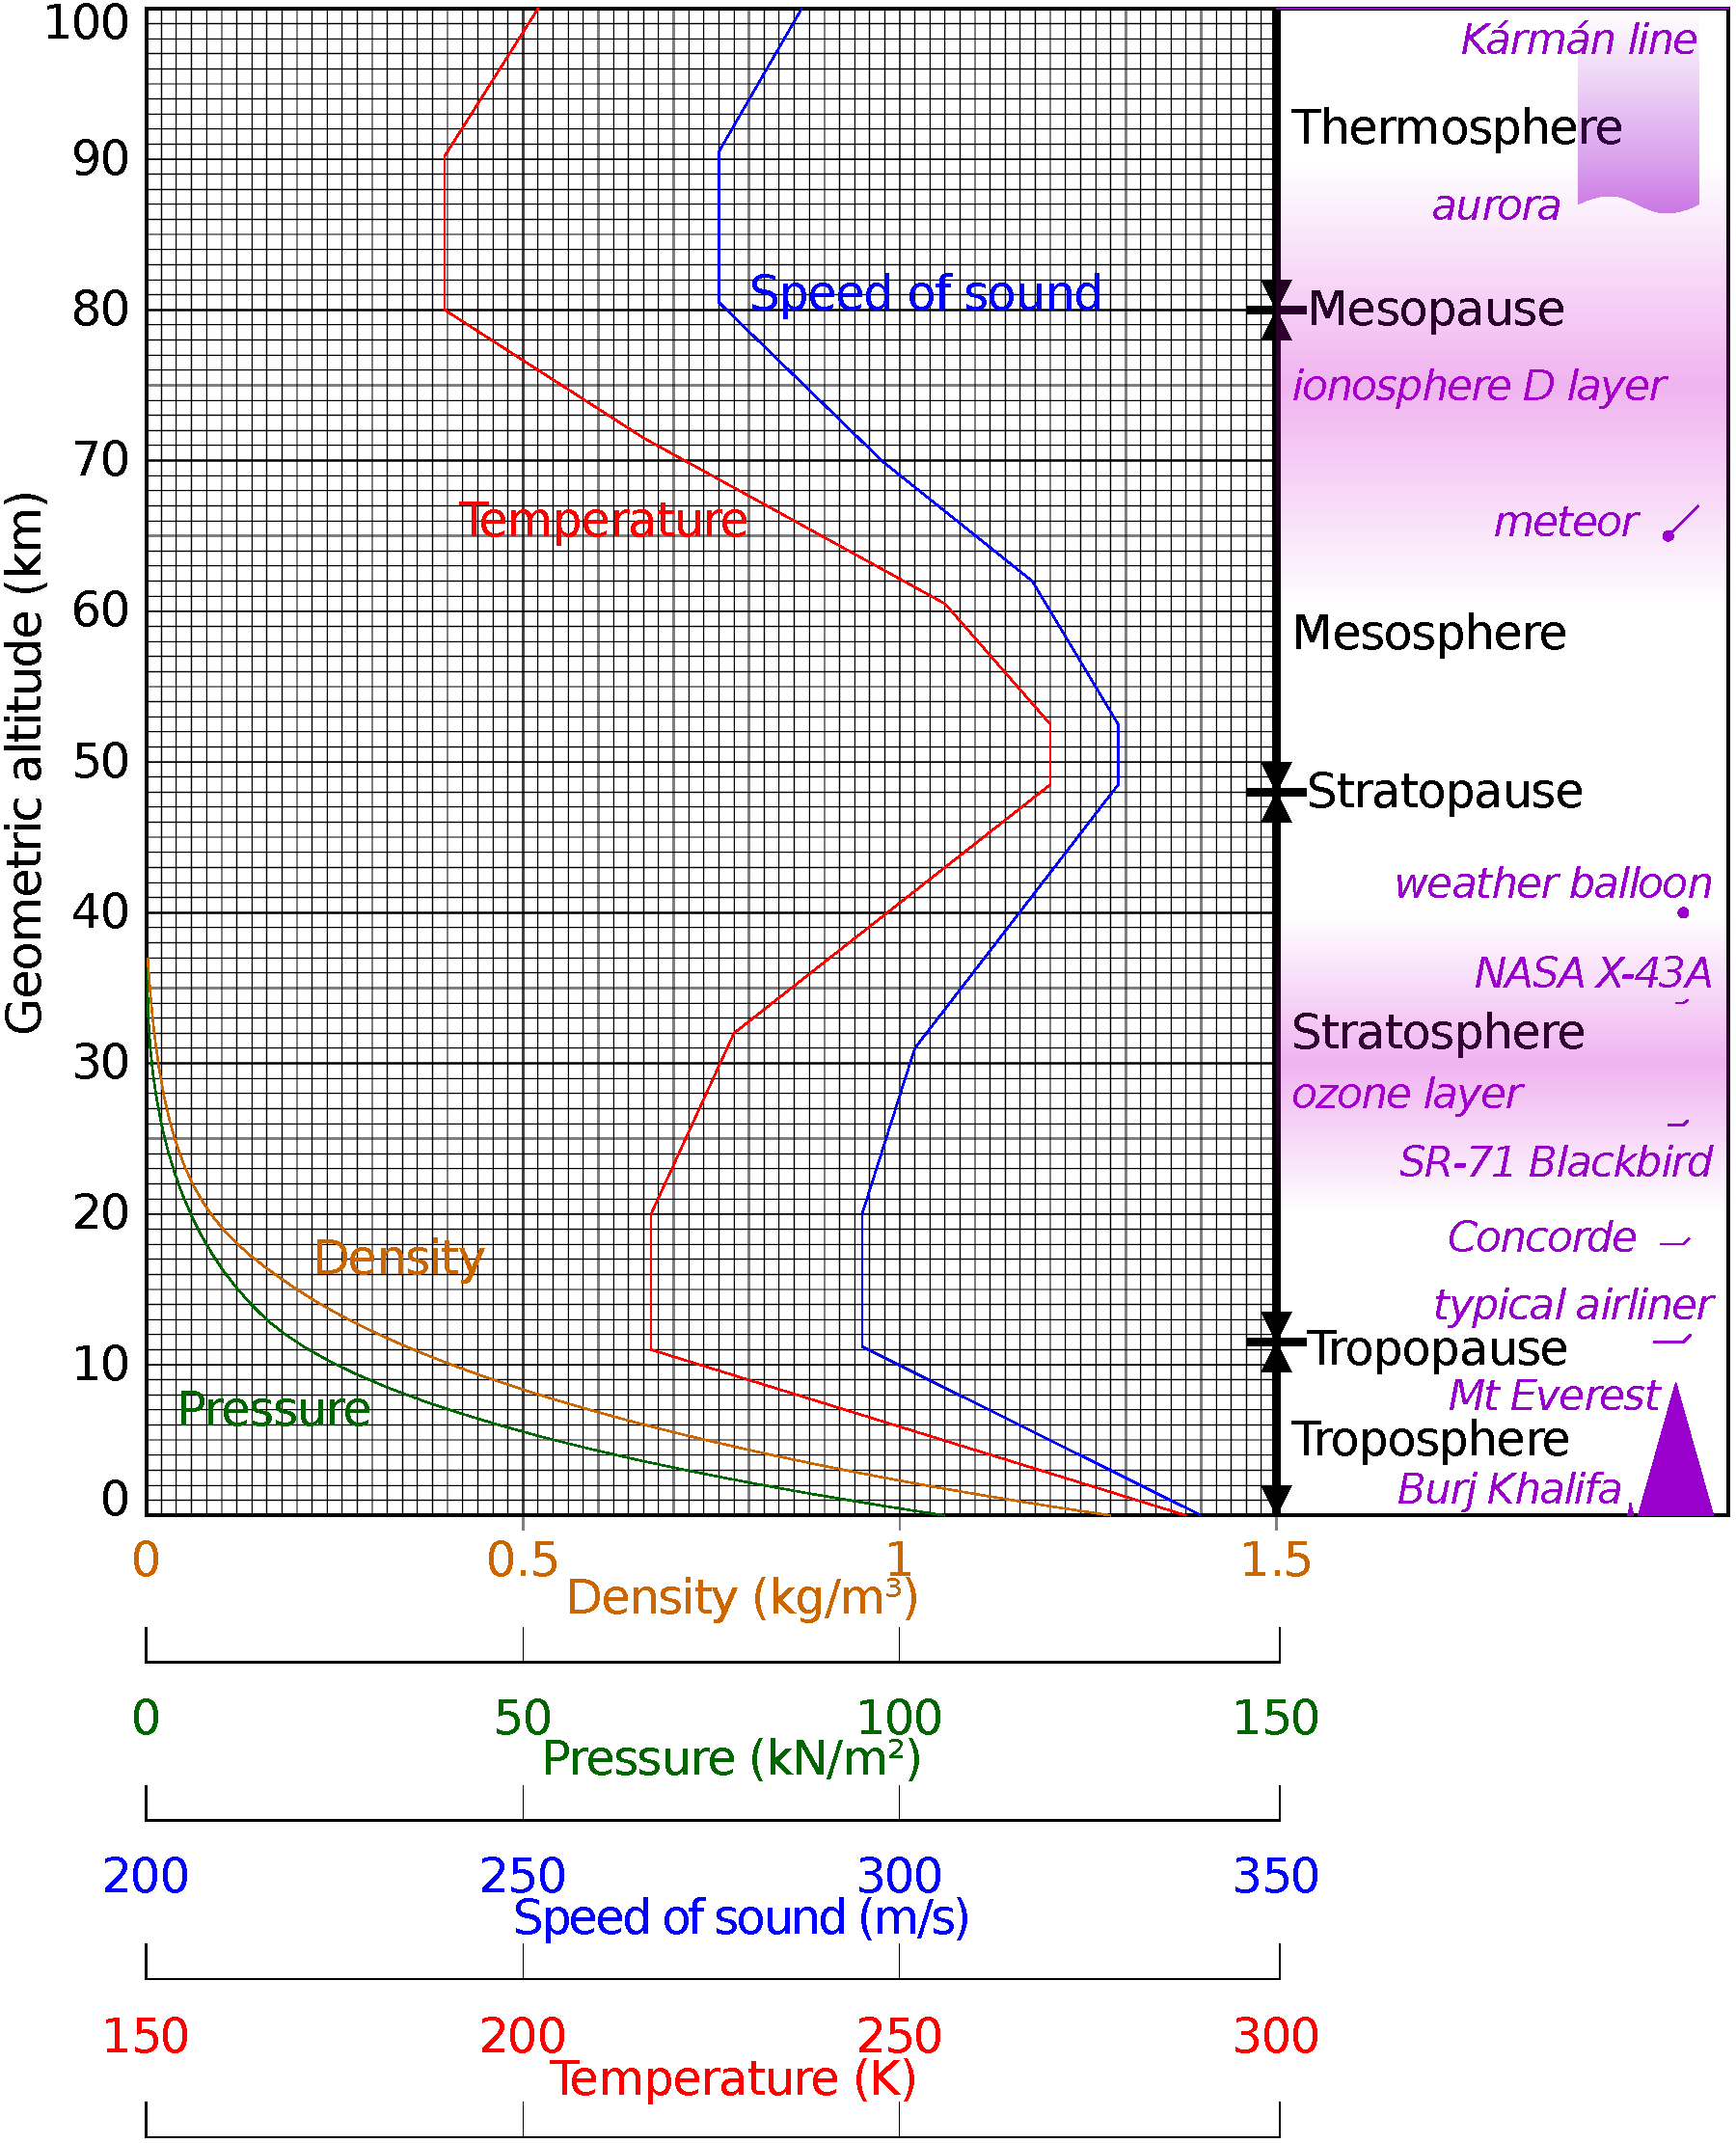
\includegraphics[width=0.6\linewidth]{chapter01/Comparison_US_standard_atmosphere_1962.pdf}
    \caption{%
        Comparaison des variables atmosphériques selon l'atmosphère standard définie par
        l'\textit{US standard atmosphere} de 1962.
        Source:
        \href{https://commons.wikimedia.org/wiki/File:Comparison_US_standard_atmosphere_1962.svg}{wikicommons},
        par \href{https://commons.wikimedia.org/wiki/User:Cmglee}{Cmglee}, CC-BY-SA.
    }%
    \label{fig:chapter01/Comparison_US_standard_atmosphere_1962}
\end{figure}

\subsubsection{La couche limite atmosphérique}%
\label{sub:la_couche_limite_atmospherique}

À l'intérieur de cette fine couche d'environ \SI{600}{km}, seule la troposphère,
c'est-à-dire les 13 premiers kilomètres, nous est directement familière. C'est en effet
dans la troposphère que les phénomènes météorologiques auxquels nous sommes habitués s'y
déroulent : nuage, vent, pluie, etc. Alors que l'atmosphère paraît immense, il est
important de noter la faible hauteur de cette couche.

La partie de la troposphère directement impactée par les effets de la surface terrestre
(friction, réchauffement, turbulence) est appelée la couche limite atmosphérique (CLA, ou
\textit{atmospheric boundary layer (ABL))}. Cette couche variant de quelques dizaines à centaines
de mètres selon les lieux et périodes de la journée, a une dynamique rapide et
convective. Notamment intéressant pour cette thèse, cela a pour conséquences que les
émissions de surface anthropiques ou naturelles, et notamment les polluants, sont
redistribuées sur l'intégralité de cette hauteur.

Durant la nuit, la hauteur de la CLA est faible du fait de l'affaiblissement du
gradient thermique vertical lié à l'absence de réchauffement radiatif du sol (voir
Figure~\ref{fig:chapter01/Atmospheric_boundary_layer}) et la mise en place de la couche de
surface après le coucher du soleil. À l'aube, la surface se réchauffe et la
convection se met en place, rendant la CLA beaucoup plus homogène et diluant gaz et
particules dans un plus gros volume d'air. Les composés ne traversent cependant que
rarement la couche d'inversion thermique, limite entre la CLA et la troposphère libre.
Ainsi, après le coucher du soleil, on observe fréquemment une couche résiduelle au milieu de
la CLA qui ``capture'' les composés d'une journée à une autre.

Il est à noter que des couches d'inversions thermiques à plus basse altitude peuvent se
mettre en place, notamment dans les vallées alpines. Pour un flux d'émission
constant, cela entraîne donc une accumulation forte des composés chimiques dans un volume
très restreint, augmentant mécaniquement les concentrations.
\cite{allardQualite2018} a ainsi pu montrer que le gradient thermique est l'un des
facteurs explicatifs le plus important pour la compréhension des concentrations en
vallées alpines.
%Notamment, certains jours à Passy, France, un facteur de concentration de 700 était présent entre 

\begin{figure}[h]
    \centering
    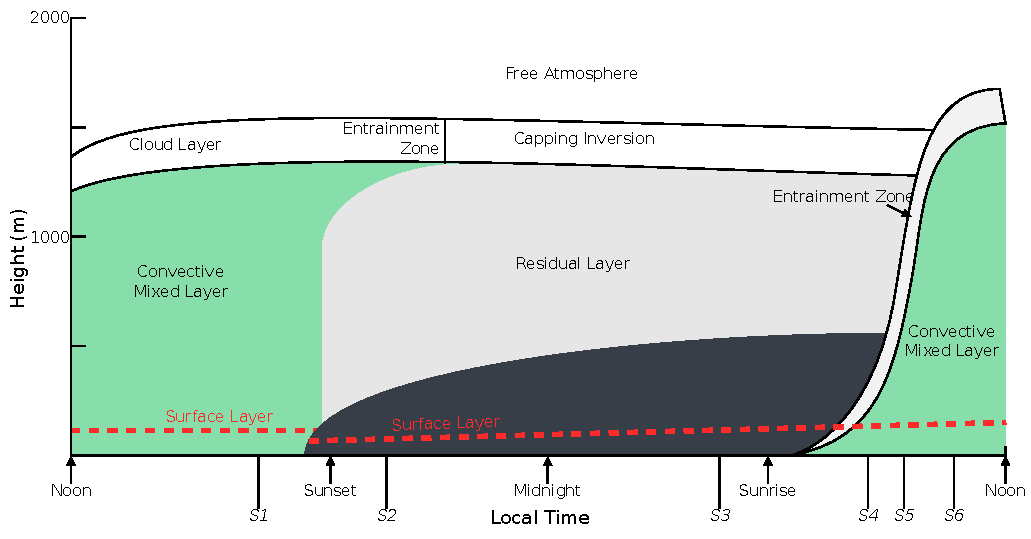
\includegraphics[width=0.8\linewidth]{chapter01/Atmospheric_boundary_layer.pdf}
    \caption{Évolution journalière schématique de la couche limite atmosphérique.
        Credit: By
        \href{https://commons.wikimedia.org/w/index.php?curid=18862904}{NikNaks} - Own
        work based on:
        \url{http://ars.sciencedirect.com/content/image/1-s2.0-S0360128504000371-gr4.jpg}.
        See also: \url{http://www.archaeocosmology.org/eng/tropospherelayers.htm}., CC
        BY-SA 3.0
    }%
    \label{fig:chapter01/Atmospheric_boundary_layer}
\end{figure}


\section{Les aérosols atmosphériques}%
\label{sec:les_aerosols_atmospheriques}

\subsection{Qu'est-ce qu'un aérosol?}%
\label{sub:quest-ce-quun-aerosol}

L'air que nous respirons est constitué majoritairement de gaz (\ce{N2}, \ce{O2}…) mais
également de particules solides ou liquides en suspension dans l'air. Très
légères et de tailles de l'ordre du nanomètre à quelques dizaines de micromètres,
ces particules sont communément appelées particules fines, ou \textit{particulate matter} (PM).

À titre de comparaison, cela reviendrait à grouper dans une même catégorie une marche de
\SI{100}{m} pour aller chercher son pain à un voyage de \SI{10000}{km}.
Ainsi, cette nomenclature ``PM'' regroupe nécessairement des objets aux caractéristiques
très diverses, comme le montre la Figure~\ref{fig:aerosolDistribution}. Selon
que l'on observe les PM en s'intéressant à leur nombre, surface ou volume, l'importance
relative des classes de taille change complètement.

\begin{figure}[ht]
    \centering
    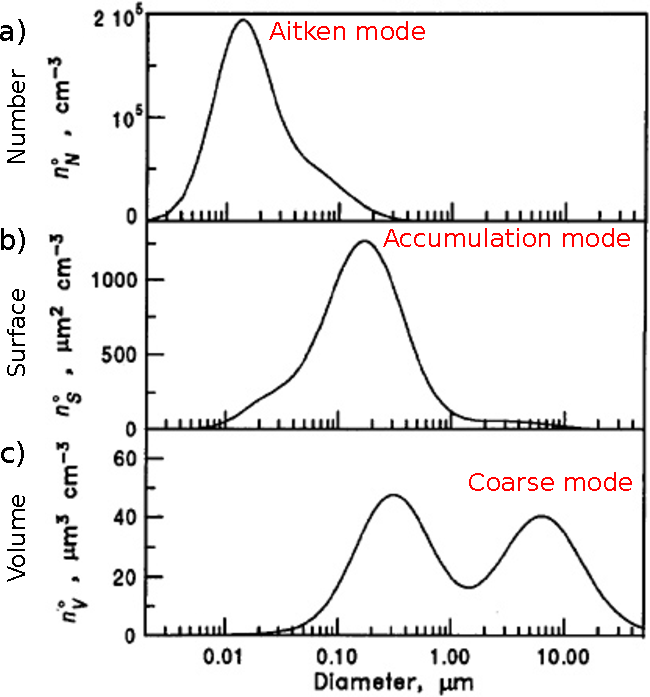
\includegraphics[width=0.5\textwidth]{aerosolDistribution.pdf}
    \caption{Distribution \textbf{(a)} en nombre, \textbf{(b)} surface, et
        \textbf{(c)} volume, pour un ensemble typique de distribution trimodale
        d'aérosols. Figure adaptée du livre de~\cite{seinfieldAtmospheric1998}.}
    \label{fig:aerosolDistribution}
\end{figure}

Ces différentes classes de taille (appelées modes) sont dues à différents procédés à
l'origine de leurs présences dans l'air. Le mode le plus fin et prépondérant en nombre,
dit d'Aikten, correspond à la nucléation à partir de composés gazeux ou de sources de
combustion.  Par coagulations successives et transformations dans les nuages, des
particules plus grosses se forment (mode d'accumulation).  Enfin se forme le mode grossier
alimenté par diverses autres sources comme la remise en suspension de poussières ou sable
par le vent, les pollens, les activités humaines, parmi d'autres, comme nous le verrons
plus loin.

La nomenclature des aérosols est ainsi historiquement fondée sur leur taille:
\begin{itemize}
    \item \PMdix, dont le diamètre aérodynamique est inférieur ou égal à \SI{10}{\um} (petit
        grain de sable, pollens…)
    \item \PMdc, dont le diamètre aérodynamique est inférieur ou égal à \SI{2.5}{\um}
        (suie, fumée…)
    \item \PMun, parfois appelé particules ultrafines (UFP), dont le diamètre
        aérodynamique est inférieur ou égal à \SI{1}{\um} (coagulation et condensation de
        vapeur…)
\end{itemize}


Ces catégories très diverses présentent ainsi des formes variées, comme illustré par les
clichés de microscopies électroniques présentés figure~\ref{fig:micrography}. On retrouve
des particules sphériques de petites tailles, des formes plus géométriques issues de
processus de cristallisation comme le sel marin, etc.

\begin{figure}[ht]
    \centering
    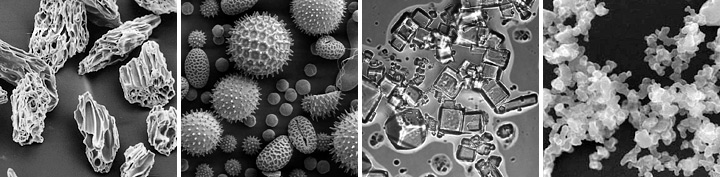
\includegraphics[width=1.0\textwidth]{aerosol_micrographs.jpg}
    \caption{Image au microscope électronique à balayage, à des échelles différentes,
        illustrant la diversité de forme des aérosols.
        De gauche à droite : cendre volcanique, pollen, sel de mer et suie. Micrographies de
        l'USGS, UMBC (Chere Petty) et de l'Arizona State University (Peter Buseck). 
        Crédit : NASA earthobservatory \url{https://earthobservatory.nasa.gov/Features/Aerosols/}.
    }
    \label{fig:micrography}
\end{figure}

\subsection{Composition chimique}%
\label{ssub:composition_chimique}

Les espèces chimiques constitutives des PM sont regroupées en différents groupes. La
figure~\ref{fig:chapter01/composition_chimique} présente les gammes de concentrations
observées à travers le monde pour différentes typologies de sites de prélèvement.
On y trouve divers ions issus de la condensation de la phase gazeuse : nitrate \NOt{} formé à
partir des \ce{NO_x}; ammonium \NHq{} formé à partir de \NHt; sulfate \SOq{} formé par
condensation et réaction chimique du \ce{SO2}.
Une part importante de la masse provient de la matière carbonée, notée ici
carbone organique (ou \textit{organic carbon} OC). Ce terme regroupe un nombre extrêmement
important d'espèces chimiques comportant une chaîne carbonée, de l'oxygène et
de l'azote. On y trouve par exemple la cellulose ou autres sucres issus de sa
dégradation par combustion (lévoglucosan, mannosan, galactosan), des ``polyols'' (arabitol,
mannitol, etc) émis par les bactéries ou champignons~\autocite{samakePolyols2019}, ou encore
d'autres familles de molécules comme les alcanes, hopanes, composés aromatiques
polycycliques ou pesticides. Cette matière carbonée est souvent nommée matière
organique (MO, ou \textit{organic matter} OM) afin de prendre en compte la masse du
carbone et celles des autres atomes (oxygène, azote…). Le facteur correctif entre OC et OM
varie entre 1.2 et 2.3 suivant les lieux de prélèvement.
Mais le carbone est également présent sous forme plus ``pure'' (i.e. avec très peu
d'oxygène ou autres atomes).
On parle alors de carbone élémentaire (\textit{elementary carbon} EC) lorsqu'il est mesuré
par méthode thermique, et de carbone noir (\textit{black carbon} BC) lorsqu'il est mesuré
par méthode optique. Cette distinction EC ou BC provient du fait qu'il existe un continuum
entre le carbone organique et le carbone élémentaire, et chacune des méthodes
d'observation implique un seuil différent de séparation entre ces deux catégories.
Pour finir, d'autres ions sont également présents, comme le sodium \ce{Na^+}, le chlore
\ce{Cl-}, le magnésium \ce{Mg^2+}, etc. mais également de nombreux éléments métalliques
comme le cuivre \ce{Cu}, l'aluminium \ce{Al}, le titane \ce{Ti}, le calcium \ce{Ca}, le fer
\ce{Fe}, etc.

La composition chimique d'un aérosol dépend de ses sources d'émissions
(voir~\ref{sub:profile_chimique_des_sources_d_émissions_courantes}) mais également des
différents processus bio-physico-chimiques présents dans l'atmosphère. Sous l'effet des
radiations solaires, de la capacité oxydante de l'atmosphère ou des micro-organismes
vivant dans l'air, la composition chimique des aérosols évolue au cours de leurs vies.
Lorsque les espèces chimiques constituant les aérosols sont identiques à celles émises par
les différentes sources d'émission, on parle d'\textit{aérosol primaire}. En revanche,
lorsque les aérosols ont subi différentes modifications et présentent de nouvelles espèces
chimiques, on parle d'\textit{aérosol secondaire}.

Cette sensibilité aux sources d'émission explique en partie la variabilité observée pour la
composition chimique et sa sensibilité à la typologie du site d'étude. Par exemple, les
sites marins présentent davantage de sels marins, les sites proches des déserts de sable
ont davantage de poussières minérales, les sites urbains ont plus de marqueurs de
combustions (EC), etc.

\begin{figure}[ht]
    \centering
    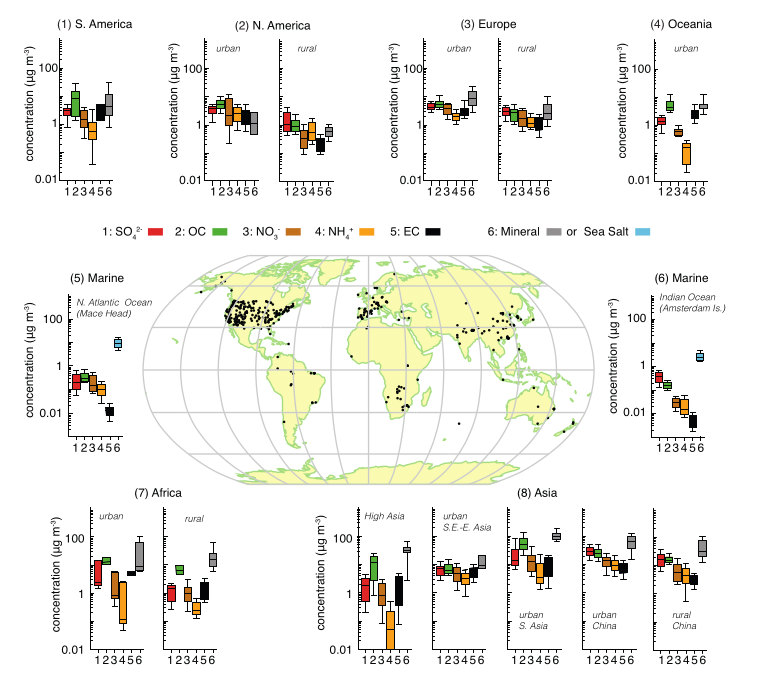
\includegraphics[width=1.0\linewidth]{chapter01/composition_chimique.png}
    \caption{Composition chimique majeure de la masse des \PMdix{} pour différentes
        typologies de sites de prélèvement. Crédit: \cite[figure 7.13]{boucherClouds2013},
        agrégeant 113 études sur au moins une année de prélèvement, entre 1993 et 2012.}%
    \label{fig:chapter01/composition_chimique}
\end{figure}

\subsection{Impacts des aérosols sur l'écosystème terrestre}%
\label{sub:impacts_des_aérosols_sur_l_écosystème_terrestre}

\subsubsection{Impacts climatiques}%
\label{ssub:impacts_climatiques}

Les aérosols sont des éléments essentiels de la machine climatique terrestre de par leur
interaction avec le rayonnement solaire et donc leur impact sur le bilan radiatif de la
Terre. Ils sont également essentiels de par leur interaction très forte avec la dynamique
des nuages, au point que les rapports du GIEC traitent dans le même chapitre les nuages et
les aérosols.

\paragraph{Impact radiatif}%
\label{par:impact_radiatif}

De par leur faible taille, les aérosols diffusent le rayonnement incident. Ils agissent
donc comme ``bouclier thermique'', ré-émettant une partie du flux solaire entrant dans
l'espace, conduisant ainsi à un refroidissement de l'atmosphère.  Cependant, les aérosols
absorbent aussi une partie du rayonnement incident, ce qui augmente l'agitation thermique
et donc conduit à un réchauffement du climat.  Ces deux effets antagonistes agissent de
concert à différentes altitudes de l'atmosphère et dépendent de la composition chimique
des aérosols.  Enfin, le dépôt des aérosols et notamment du \textit{black carbone} sur la
neige ou les glaces des banquises induit un effet bien connu de rétroaction positive. Le
carbone diminue l'albédo et absorbe le rayonnement normalement réémis par les surfaces
blanches, augmente donc localement la température et fait fondre la glace, découvrant
ainsi des surfaces plus sombres (roche ou océan) absorbant davantage de rayonnement,
conduisant à un réchauffement accru, et ainsi de suite.

\paragraph{Impacts sur la dynamique des nuages}%
\label{par:noyaux_de_condensation_des_nuages}

Les aérosols, grâce à leur taille et leurs ions, permettent en revanche de baisser
l'énergie d'activation nécessaire à l'agrégation de la vapeur d'eau sous forme liquide en
gouttelettes, puis goutte, facilitant l'apparition des nuages. Ainsi, les aérosols agissent
comme noyaux de condensation des nuages (CCN pour \textit{cloud condensation nuclei}).
Certes, les nuages empêchent les infrarouges terrestres de repartir vers l'espace, mais
présentent également un albédo élevé renvoyant une grande partie du rayonnement à courte
longueur d'onde du Soleil vers l'espace. L'effet observé est donc un refroidissement de
l'atmosphère.
Aussi, pour une même quantité d'eau, le nombre de CCN disponibles conditionne la taille des
gouttelettes des nuages donc la taille de ceux-ci, leur durée de vie et probabilité de se
transformer en nuage précipitant.

\paragraph{Impacts sur le dérèglement climatique en cours}%
\label{par:impacts_sur_le_dereglement_climatique_en_cours}

Du fait de ces différents aspects antagonistes, très brièvement exprimés ci-dessus,
l'impact total des aérosols sur le climat n'est connu qu'avec une incertitude élevée. 

La contribution des aérosols à la différence du forçage radiatif entre 1750 et 2011 s'estime entre
\SIrange[range-phrase=~et~]{-0.77}{0.23}{\W\per\m\squared} (pour un forcage total actuel
de \SI{2.29}{\W\m\squared}), avec un forçage négatif pour
les poussières minérales, le sulfate, nitrate et carbone organique, mais positif pour le
carbone suie.  Quant à leur rôle sur la dynamique des nuages, il s'estime entre
\SIrange[range-phrase=~et~]{-1.33}{-0.06}{\W\per\m\squared}, mais présente des
incertitudes plus élevées du fait de la complexité à prendre en compte ces phénomènes dans
les modèles de climat. C'est actuellement le forçage radiatif le moins bien connu de la
machine climatique Terrestre.

\subsubsection{Impacts environnementaux}%
\label{ssub:impacts_environnementaux}

La durée de vie des aérosols dans l'atmosphère entre leur émission et leur déposition est
de plusieurs jours pour la majorité d'entre eux. Dans ce délai, la circulation atmosphérique les déplace sur des
distances pouvant atteindre plusieurs milliers de kilomètres. Il n'est pas rare par exemple en
Europe d'avoir des épisodes de dépôts de sable provenant du désert saharien. Ce
déplacement longue distance d'aérosols est même un des mécanismes clef de certains
\textit{bloom}
de phytoplancton, en apportant d'importantes quantités de nutriments à la surface de l'océan 
(métaux et phosphate notamment).
Autre exemple marquant, le nitrate, élément limitant de la croissance des
plantes en prairie d'altitude, est apporté en partie par
déposition de nitrate d'ammonium particulaire provenant du transport longue
distance~\autocite{bourgeoisFoliar2019}.

Plus spectaculaire, les cendres volcaniques relarguées dans l'atmosphère suite à de
violentes éruptions, en plus de leur impact climatique potentiel, peuvent occasionner des
pluies acides du fait de la présence en quantité de sulfate dans ces cendres.

Ces phénomènes présentent à quel point les aérosols et leur composition chimique variée
impactent directement de nombreux écosystèmes terrestres, et ce, qu'ils proviennent de sources
anthropiques comme c'est le cas pour le nitrate, ou de sources naturelles.

\subsection{Impacts sanitaires}%
\label{sub:impacts_sanitaires}

L'impact sanitaire des aérosols sur la population humaine a commencé à être
un sujet de recherche suite à l'industrialisation et aux épisodes de ``smog'' causant la
mort de nombreuses personnes à Engis (Meuse, Belgique) en 1930, Donora (Pennsilvanie, USA)
en 1948 ou encore le plus connu ``Great smog of London'', en 1952. Durant ces épisodes de
pollutions, il est important de noter que la sur-mortalité due à l'exposition aigüe
durant l'épisode est très importante (jusqu'à 3 fois supérieure à la normale
pour le smog de Londres), mais que la surmortalité persiste dans les mois qui suivent
--pendant près d'un an pour le smog de Londres-- alors même que les niveaux de pollution
étaient revenus à leurs états antérieur à décembre 1952 \autocite{bellReassessment2001}.  Ces
épisodes de pollution intenses marquent le début de la prise de conscience par la
population de la problématique de la pollution de l'air et ont conduit à la première
législation anglaise en matière de qualité de l'air en 1956 avec le \textit{Clean Air
Act}. Aussi, des programmes de mesures de la qualité de l'air pour différents polluants
ont émergés et les actions misent en œuvre au niveau national et international ont permis
en depuis Europe une amélioration très sensible de la qualité de l'air
(Figure~\ref{fig:chapter01/tendance_polluants}).

\begin{figure}[ht]
    \centering
    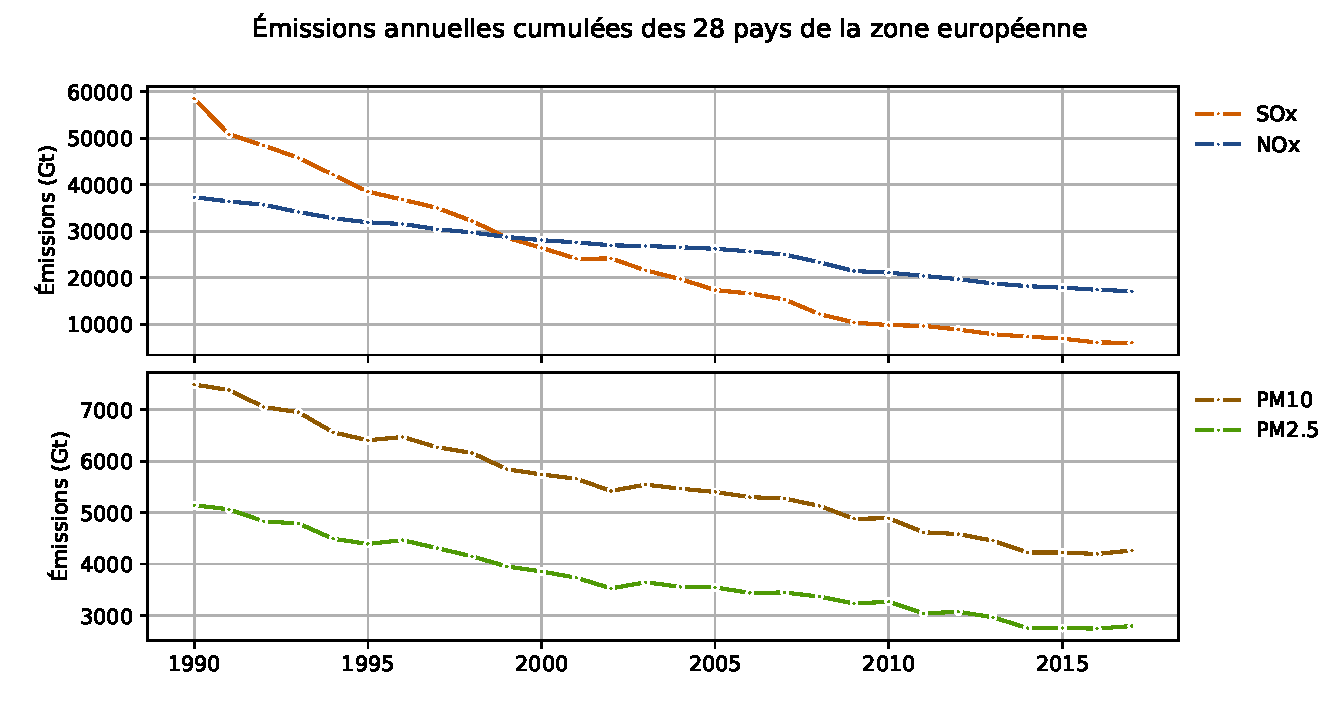
\includegraphics[width=0.9\linewidth]{chapter01/tendance_polluants.pdf}
    \caption{Évolution temporelle des émissions cumulées des 28 pays de la zone européenne
    depuis 1990, indiquant une prise de conscience et une diminution des émissions de
    différents polluants gazeux (\ce{SO_x} et \ce{NO_x}) et particulaires (\PMdix{} et \PMdc). Données
issues de \textit{National emissions reported to the Convention on Long-range
Transboundary Air Pollution (LRTAP Convention)}, ©European Environment Agency (EEA).}%
\label{fig:chapter01/tendance_polluants}
\end{figure}


Cependant, la qualité de l'air (incluant les aérosols, mais également les
composés gazeux comme les \ce{NO_x} ou l'ozone) demeure actuellement la 5\ieme{} cause de
mortalité dans le monde, représente un décés sur dix et est catégorisée ``cancérogène
certain'' par le CIRC depuis 2013. En Europe, pour l'année 2013, c'est
ainsi \num{800000} personnes qui sont décédées des suites de maladies cardiovasculaires,
cancer, pneumonie… directement attribuables à la qualité de l'air
\autocite{worldhealthorganizationAmbient2016}. Récemment, \cite{lelieveldLoss2020}
estiment qu'en moyenne et à travers le monde, c'est \num{2.9} ans de vie perdue par personne
qui sont imputables à la pollution de l'air, dont \num{1.7} ans ``évitables'' car provenant
directement de sources anthropiques.

En termes de bilan financier, la banque mondiale en collaboration avec l'Institute for
Health Metrics and Evaluation (IHME) de l'université de Washington estimait que le coût
associé aux décés prématurés de la seule année 2013 s'évaluait à plus de \$5.11 trillions
de dollar dans le monde~\autocite{worldbankCost2016}.

Afin de limiter cet impact sanitaire, de nombreux pays ont définis des seuils de
concentrations de différents composés (voir Tableau~\ref{tab:seuil_PM} pour les PM).
Seulement ces seuils sont différents d'une institution à une autre. Par exemple, entre
2015 et 2017, le seuil de concentration journalière recommandé pour les \PMdix{} par
l'union européenne (\SI{50}{\ugm} en moyenne journalière) était dépassé pour 13 à
19~\% de la population européenne, mais cette proportion augmente entre 42 et 62~\% si
l'on prend en compte le seuil recommandé de l'OMS de \SI{20}{\ugm} en moyenne
annuelle~\autocite{europeanenvironmentagencyAir2019}.  De plus, il est à noter qu'il
n'existe pas de seuil à partir duquel l'exposition aux PM est inoffensive.

\begin{table}[ht]
    \begin{ThreePartTable}
        \centering
        \caption{Seuils de concentration de PM recommandés par différents organismes.}
        \label{tab:seuil_PM}
        \begin{tabular}{ccSc}
            \toprule
            Organisme       & Polluant & {Concentration (\si{\ugm})} & Période \\
            \midrule
            OMS\tnote{a}    & \PMdc  & 10 & moyenne annuelle       \\
            OMS\tnote{a}    & \PMdc  & 25 & moyenne sur \SI{24}{h} \\
            OMS\tnote{a}    & \PMdix & 20 & moyenne annuelle       \\
            OMS\tnote{a}    & \PMdix & 50 & moyenne sur \SI{24}{h} \\
            Europe\tnote{b} & \PMdc  & 25 & moyenne annuelle       \\
            Europe\tnote{b} & \PMdc  & 20 & moyenne sur 3 ans      \\
            Europe\tnote{b} & \PMdix & 40 & moyenne annuelle       \\
            Europe\tnote{b} & \PMdix & 50 & moyenne sur \SI{24}{h} \\
            France\tnote{c} & \PMdc  & 25 & moyenne annuelle       \\
            France\tnote{c} & \PMdix & 50 & moyenne sur \SI{24}{h} (\SI{<35}{jour\per an}) \\
            France\tnote{c} & \PMdix & 40 & moyenne annuelle \\
            \bottomrule
        \end{tabular}
        \begin{tablenotes}
        \item[a] OMS air quality guideline \cite{worldhealthorganizationWHO2006}
        \item[b] Directive 2008/50/EC \cite{officialjournaloftheeuropeanunionDirective2008}
        \end{tablenotes}
    \end{ThreePartTable}
\end{table}

\section{Détermination des sources d'émission des PM}%
\label{sec:source_apportionment_of_pm}

Comme nous l'avons vu, les sources d'aérosols sont très diverses.
Afin de pouvoir avoir un impact sur les concentrations de polluants via des
réglementations, il est primordial de
retracer leur provenance. Plusieurs techniques d'analyses existent, qu'elles soient purement
physiques ou géochimiques.

\subsection{Modèle d'attribution des sources}%
\label{sec:source_apportionment_model}

Afin d'estimer la contribution de chaque source de PM en un point donné, il est possible
d'utiliser 2 grandes familles de modèles d'attribution des sources (\textit{source
apportionment} (SA)). La première est fondée sur notre connaissance des
émissions et de la météorologie et calcule les réactions physico-chimiques depuis les
sources jusqu'au lieu d'étude (modèle dit de chimie-transport (\textit{chemical transport
model} (CTM)) alors que la deuxième s'évertue à mesurer en un point donné
la chimie des PM et par traitement statistique, attribue à différentes sources ou
``facteurs'' leurs contributions aux concentrations observées (modèle dit récepteur
(\textit{receptor model} RM)).

\subsubsection{Modèle déterministe de chimie-transport}%
\label{ssub:modele_deterministe_de_chimietransport}

\paragraph{Présentation}%
\label{par:presentation}

Les modèles déterministes s'appuient sur l'inventaire des sources d'émissions sur la
région étudiée. Ces cadastres d'émissions sont regroupés en catégories \textit{Selected
Nomenclature for reporting of Air Pollutants} (SNAP) représentant chacune un secteur
d'activité : Énergie, Procédés industriels, Agriculture, Déchets, Autres et enfin
Naturelle.
Chacune de ces catégories possédant évidemment des sous-catégories raffinant la
classification (par exemple, les émissions de l'aviation civile des avions de plus de \SI{100}{m} de
long se retrouvent dans le SNAP 080503 (ou \textit{Nomenclature For Reporting} (NFR)
1.3.A.c) autrement dit Énergie - Combustion - Aviation - Aviation civile de plus de
\SI{100}{m})~\autocite{europeanenvironmentagencyEMEP2019}.
À chacune de ces SNAP est associé un profil d'émission (\ce{O3}, \ce{SO2}, \ce{NO_x}, \ce{NH3}, \PMdix, \PMdc,
VOC principalement), obtenu soit par mesure directe, soit par calcul.

Vient ensuite un inventaire de ces sources d'émissions sous forme de cadastre géographique
et temporel. Notamment la \textit{Convention on Long-Range Transboundary Air
Pollution} (LRTAP) implémenté par l'\textit{European Monitoring and Evaluation Program}
(EMEP) sous l'égide de \textit{United Nations Economic Commission for Europe} (UNECE)
prévoit que les différentes parties prenantes à cette convention (i.e. les pays membres)
présentent un rapport de leurs émissions régulièrement à l'EMEP.

Il est alors possible de construire des modèles déterministes de dispersion et de
réaction des polluants, en couplant un modèle de diffusion résolvant les équations de la
physique de l'atmosphère (Navier-Stoke, turbulence, rayonnement, etc) avec un modèle
physico-chimique faisant évoluer les composés gazeux et particulaires, incluant leurs
émissions, dépôts, interaction physico-chimique, etc. Pour n'en citer que quelques-uns : 
Community Multi-scale Air Quality (CMAQ)\footnote{CMAQ: \url{https://www.epa.gov/cmaq}},
Comprehensive Air Quality Model with Extensions (CAMx)\footnote{CMAx : \url{http://www.camx.com/}},
WRF-Chem\footnote{WRF-chem : \url{https://www2.acom.ucar.edu/wrf-chem}},
Chimère,
LOTOS-EUROS...

La raison de la pluralité de ces modèles provient des différentes paramétrisations
possibles des équations physiques, mais également des choix conceptuels de recherche.

\paragraph{Limitations}%
\label{par:limitations}

Comparaison Chimire-DECOMBIO : \cite{bessagnetHigh2020}
\todo{à faire}

\paragraph{Source apportionment}%
\label{par:source_apportionment}

Concernant l'attribution des sources, il est possible d'utiliser deux techniques au sein
des CTM:

\begin{enumerate}
    \item Faire une première simulation incluant toutes les sources d'émissions (référence
        ou témoin), puis une deuxième simulation avec une source d'émission en moins. La
        différence reflétant l'impacte de la source supprimée sur les concentrations
        ambiantes (technique dite de force-brute);
    \item Garder en mémoire la provenance de chacune des espèces chimiques lors des
        schémas réactionnels (technique dite de \textit{source labelling} ou \textit{tagged species}).
\end{enumerate}

Seulement, du fait des nombreux processus non linéaires, la suppression d'une source
d'émission aura des répercussions beaucoup plus complexes que la simple diminution des
concentrations propres à cette source (par exemple, des NOx pourraient ne pas passer en
phase particulaire du fait d'un manque d'ammoniac, ou inversement). 
% TODO: élaborer ou supprimer cette partie
%La première technique correspond donc à se demander 
%\begin{quote}
%    Si les émissions de cette source sont diminuées ou supprimées, quels impacts cela va-t-il
%    avoir sur les concentrations finales ?
%\end{quote}
%alors que la deuxième répond à
%\begin{quote}
%    Dans la concentration ambiante de PM, à combien s'estime la contribution de cette source
%    d'émission ?
%\end{quote}
%Ce sont bien deux questions différentes avec leurs légitimités propres.
La seconde technique a commencé été implémentée plus récemment dans certains
CTM~\autocite{wangDevelopment2009,wagstromDevelopment2008,kranenburgSource2013,brandtContribution2013}
et elle est détaillée dans le rapport de~\cite{mirceaEuropean2020}. Elle présente également
l'avantage de pouvoir tagguer non seulement les sources des espèces chimiques, mais
également leur provenance géographique, c'est-à-dire leur lieu d'émission.

Cependant, l'utilisation des CTM présente certaines limites du fait de leur complexité.
Notamment, il semble illusoire de pouvoir un jour inclure toutes les réactions chimiques
possibles dans les modèles déterministes. Par exemple, les interactions aérosols/neiges ou
même plus simplement les interactions aérosol nuages et la chimie aqueuse qui s'y produit
ne sont pas encore complètement comprises ni bien représentées dans ces modèles.

Quand bien même ce serait le cas --car les modèles réactionnels sont de plus en plus
poussés--, il faudrait alors avoir des inventaires d'émissions beaucoup plus complets et
précis temporellement, avec aucune certitude d'un oubli potentiel d'une source non prise
en compte. Ce sont par exemple, une industrie locale non-encore répertorié, la sous-estimation de
la contribution d'un écosystème, une consommation de bois de chauffage individuel non
inventoriée, etc.

Aussi, la limitation physique des modèles météorologiques se retrouvent dans les CTM. Il
est donc compliqué d'envisager, du fait du coût de calcul et de stockage, une simulation à
\SI{10}{\m} de résolution spatiale (ou moins), ce qui serait cependant nécessaire pour
appréhender correctement des phénomènes précis, comme les inversions thermiques des
vallées alpines.

\subsubsection{Modèles récepteurs}%
\label{ssub:model_recepteur}

À l'inverse des CTM, il est possible d'estimer les sources contribuant aux concentrations
ambiantes en un lieu donné sans la moindre information météorologique ou simulation
déterministe. Pour cela, il convient de faire des prélèvements sur le lieu d'étude,
d'analyser la chimie que l'on y trouve et retrouver à l'aide d'un modèle statistique
les différents profils de source et leurs contributions, ce qui peut se traduire en
particulier par l'équation d'équilibre des masses
\begin{align}
    \label{eq:mass_balance}
    X &= G \cdot F
\end{align}
où $X$ est la matrice de dimension $n\times m$ des observations, $G$ est la matrice des
contributions de taille $n\times p$ et $F$ la matrice des profils de taille $p \times n$,
avec $n$ le nombre d'échantillons, $m$ le nombre de variables chimiques mesurées et $p$ le
nombre de facteurs.
Un \textit{facteur} peut être une source d'émission (combustion de biomasse par exemple),
mais également regrouper des espèces chimiques provenant d'un même processus secondaire
(nitrate d'ammonium par exemple).
Il est courant d'exprimer $X$ en \si{\ugm}, $G$ en \si{\ugm} ou concentration
normalisée~\si{[-]} et $F$ en \si{\micro\g\per\micro\g} ou \si{\ugm}.

Si l'on mesure $X$, ce qui nous intéresse ici est de connaître $G$ ou $F$.
Si l'on admet que l'on connait a priori les profils d'émissions possibles, alors $F$ est
connue et l'on cherche à estimer $G$. Le modèle de déconvolution adapté est alors le
\textit{Chemical Mass Balance} (CMB). À l'opposé, on peut n'avoir aucune information a
priori à la fois sur les contributions et les profils d'émissions. On utilisera alors le
modèle de déconvolution \textit{Positive Matrix Factorization} (PMF).

Ces 2 types de modèles statistiques sont aux deux extrêmes d'un spectre de modèles de
déconvolution, depuis une information ``absolue'' des profils de sources à une absence
totale d'information sur ces mêmes profils.  Il existe cependant un continuum entre ces
deux pôles (voir Figure~\ref{fig:chapter01/source_apportionment_methods}), et de nombreux
modèles ont été développés et améliorés depuis la première étude de SA de
\cite{colucciAutomotive1965} utilisant la ``simple'' corrélation entre le \ce{CO} et
le plomb et benzo(a)pyrène.  Une revue détaillée et historique du fonctionnement de ces
différents modèles peut-être retrouvées dans les articles de
\cite{henryHistory1997,vianaSource2008,belisCritical2013,hopkeReview2016}.

\begin{figure}[ht]
    \centering
    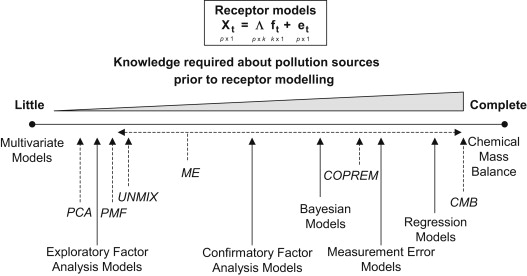
\includegraphics[width=0.7\linewidth]{chapter01/source_apportionment_methods.png}
    \caption{
        Connaissances a priori nécessaires pour les différents modèles de SA existant,
        depuis la simple analyse de facteur par ACP au modèle CMB. Crédit :
        \cite{vianaSource2008} adaptée de \cite{schauerCharacterization2006}
    }%
    \label{fig:chapter01/source_apportionment_methods}
\end{figure}

\subsubsection{Chemical mass balance CMB}%
\label{ssub:chemical_mass_balance_cmb}

Le principe du CMB est de déterminer la contribution $G$ d'un nombre de sources
aux profils chimiques $F$ prédéfinis aux concentrations ambiantes $X$. Il est donc
nécessaire de connaître les signatures chimiques des sources utilisées.

Afin d'utiliser le modèle CMB --mais également pour d'autres buts-- l'US EPA construit
depuis 1988 la base de donnée SPECIATE~\autocite{simonDevelopment2010}, répertoriant
différents profils d'émission, dont la 5\ieme{}
version a été publiée en 2019~\autocite{u.s.environmentalprotectionagencySPECIATE2019}.
Seulement, ces profils sont représentatifs des sources présentes aux États-Unis et sont
très certainement non transposables à d'autres régions du monde.
En Europe, il existe depuis 2016 une base de données similaire,
SPECIEUROPE~\autocite{pernigottiSPECIEUROPE2016}, compilant des mesures à l'émission et
les résultats d'autres types d'étude permettant d'estimer la signature chimique des
profils d'émission.

Cependant, des erreurs ou variabilités locales spécifiques au site récepteur sur ces
profils peuvent conduire à une estimation erronée des contributions finales des
différentes sources en utilisant le modèle CMB.
Aussi, il est nécessaire de choisir ou d'agréger certains des >3000 profils de sources
différents répertoriés afin de restreindre à une valeur réaliste le nombre de sources
potentielles en un lieu donné.
Enfin, les processus secondaires sont mal pris en compte dans ce type modèle. L'exemple typique
concerne l'aérosol inorganique secondaire sulfaté, représenté comme un mélange de sulfate
et d'ammonium. Or ce facteur secondaire est souvent associé en réalité à de la matière
organique ou d'autres espèces sulfatées.

\subsubsection{Positive Matrix Factor PMF}%
\label{ssub:pmf}

Un modèle beaucoup plus agnostique que le CMB pour résoudre l'équation de conservation de
la masse a été développé par~\cite{paateroPositive1994}. Dans cette formulation,
seule la matrice d'observation $X$ est connue, et les matrices de contribution $G$ et des
profils chimiques $F$ sont inconnues.

\paragraph{Formulation mathématique}%
\label{par:formulation_mathématique}

Le principe de la PMF provient initialement de la recherche sur le \textit{machine
learning}, et plus particulièrement de l'analyse factorielle appliquée au problème
bilinéaire $X=G\times F$. L'intérêt initial est de permettre une réduction
dimensionnelle sans perte d'information. Par exemple, en informatique, une image de $n$
par $m$ pixels forme une matrice $n\times m$ éléments. S'il est possible de retrouver
cette matrice par multiplication de 2 matrices $G$ ($n\times p$) et $F$ ($p \times m$),
alors la quantité d'information stockée dans $G$ et $F$ est $n
\times p + p \times m = p \times (n + m)$. Ainsi, tant que $p < \frac{n\times m}{n+m}$,
alors le nombre d'éléments de $G\times F$ est toujours inférieur au nombre d'éléments de
$X$, permettant un gain de mémoire de plus en plus important au fur et à mesure que $n$ et
$m$ augmentent.
Tout le problème réside en le fait de trouver la décomposition de $X$ en minimisant
l'erreur engendrée par cette simplification.

Aussi, on observe que la formulation $X = G\cdot F$ est similaire à celle de
la conservation de la masse (Eq.~\ref{eq:mass_balance}). Ce problème peut-être résolu par
analyse en composante principale (ACP), seulement, le résultat obtenu présente des
combinaisons linéaires (additive et soustractive) des différents composants. Cette possible
négativité des composants n'a pas de sens dans beaucoup de domaines physiques, y compris en
géochimie. \cite{paateroPositive1994} présentent donc une nouvelle méthode de
déconvolution, implémentant une contrainte de non-négativité, nommée \textit{Positive Matrix
Factorization} (PMF). 

La formulation est la suivante : étant donné une matrice d'observation $X$ de taille
$n\times m$, une matrice associée des incertitudes $U$ de taille $n \times m$ et un rang
$p$, alors 
\begin{align}
    \label{eq:pmf_formulation}
    X &= G \cdot F + E \\
    \forall i,k,j &, G_{ik}\geq 0 \text{ et } F_{kj}\geq 0\\
    Q &= \sum_{i=1}^n\sum_{j=1}^m E_{ij}^2/U_{ij}^2\label{eq:Qfunction}\\
    {Q, F} &= \argmin_{G,F} Q.
\end{align}

Différents algorithmes de résolution du système Eq.~\ref{eq:pmf_formulation} ont été développés.
L'implémentation initiale de~\cite{paateroLeast1997} a été améliorée pour pouvoir
ajouter des contraintes sur les matrices $G$ et $F$, notamment grâce au solveur
\textit{multi-linear engine} (ME-2) \autocite{paateroMultilinear1999}. En effet, il
n'existe pas de solution unique au problème Eq.~\ref{eq:pmf_formulation}, notamment, car le
système est invariant par rotation:
\begin{align}
    \label{eq:rotationalambiguity}
    X   &= G \cdot F + E \\
        &= (G \cdot T) \cdot (T^{-1} \cdot F) + E\\
        &= G' \cdot F' + E
\end{align}
et ainsi une infinité de solutions coexistent. 

\paragraph{Interprétabilité du modèle PMF}%
\label{par:interpretabilite_du_model_PMF}

L'avantage de la PMF réside en le fait que l'algorithme n'est pas fondé sur la
corrélation entre variables, comme c'est le cas de l'ACP, mais bien en la formation d'un
modèle additif linéaire de ce qui est observé.
\begin{quote}
    We shall not be satisfied in finding some correlations, we wish to form a quantitative
    model of what was observed! \autocite{paateroPositive1994}
\end{quote}

Il a été montré que la PMF est capable d'extraire des informations partielles cohérentes des
données là où l'ACP n'est qu'une représentation holistique~\autocite{leeLearning1999}. Par
exemple, appliquée à la reconnaissance d'image faciale, la PMF déconvolue les visages en
sous partie (bouche, sourcils, front, etc) alors que d'autres méthodes ``se contentent''
d'une approche globale de l'information et où seules les premières dimensions portent
l'information nécessaire à la reconstruction du signal (voir
figure~\ref{fig:chapter01/NMFvsPCA}).

\begin{figure}[ht]
    \centering
    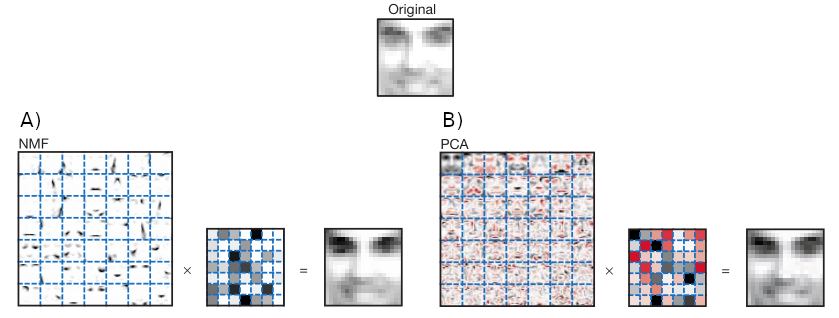
\includegraphics[width=1.0\linewidth]{chapter01/NMFvsPCA.png}
    \caption{Analyse factorielle par PMF (ou NMF pour \textit{non-negative matrix
    factorization}) et ACP d'une banque d'image de 2429 images en niveau de gris de 19
    pixels par 19 pixels. Les deux techniques essaient de reproduire l'image originale en
    fonction de leur apprentissage.
    \textbf{A)} Le rang de la PMF est $p=49$, correspondant aux 49
    représentations des $19\times19$ images à gauche, chacune étant un facteur de la
    matrice $F$, et leurs ``contributions'' respectivement identifiées par le carré de 7 par
    7 en niveau de gris, à droite.
    \textbf{B)} Analyse en composante principale, le carré de gauche représentant les 49
    vecteurs propres et celui de droite les 49 valeurs propres.
    Les échelles de couleurs sont : rouges pour les coefficients négatifs, noirs pour les
    coefficients positifs.
    Figure adaptée de \cite{leeLearning1999}}%
    \label{fig:chapter01/NMFvsPCA}
\end{figure}

\paragraph{Applicabilité en science de l'atmosphère}%
\label{par:applicabilité_en_science_de_l_atmosphère}

Dans le cas qui nous intéresse ici, cela signifie que chacun des vecteurs de la matrice
$F$ correspond à un profil chimique, en \si{\ugm}, indépendant des autres profils, et
que la matrice $G$ représente la contribution de chacun de ces profils au jour
considéré, de manière cohérente avec l'équation de conservation de la masse.

Puisque la PMF ne nous donne qu'un profil chimique, certains de ces profils représentent
directement une source d'émission, et d'autres correspondent à un ensemble de processus
conduisant à un profil chimique stable. On ne peut donc pas appeler ``source'' tous les ensembles
identifiés par la PMF puisque certains ne sont pas à proprement parler émient tels quels et
proviennent de processus physico-chimiques ayant eu lieu après les émissions de ces
composés.
Le terme de \textbf{facteur} est donc utilisé pour désigner un profil chimique et sa
contribution.

Le modèle PMF est maintenant très largement utilisé, et son application a été grandement
favorisée
par son implémentation dans le logiciel de l'EPA: EPA PMF5.0~\autocite{norrisEPA2014}.
Si l'EPAPMF5 est massivement utilisée pour les données provenant d'analyses de
filtres, l'utilisation pour des spectres de masse provenant de mesures d'AMS est facilitée par
l'utilisation du logiciel SoFi~\autocite{canonacoSoFi2013}. Ces deux logiciels utilisent
le solveur ME-2 pour résoudre le système d'équation de la PMF.

\paragraph{Estimation des incertitudes}%
\label{par:incertitudes}

Il existe différent type d'incertitudes pour ce modèle : 1) la sensibilité aux données
d'entrée (sur ou sous représentation de certains événements : impact d'un point
``extrême'' par exemple) et 2) l'incertitude rotationelle~\autocite{brownMethods2015}.

La première incertitude est évaluée à travers une méthode de \textit{bootstrap} consistant
à ré-échantilloner par blocs la matrice des observations $X$, à reconduire une simulation
PMF et à faire correspondre chacun des nouveaux facteurs obtenus à ceux qui lui sont le
plus proche dans la simulation initiale.
On obtient ainsi une incertitude sur les profils chimiques mais également sur les
contributions temporelles.
Cela permet aussi d'évaluer si la solution initiale était statistiquement peu fréquente
dans l'espace des possibles ou si au contraire elle correspond à minimum de la fonction
coût $Q$ relativement commun.

L'incertitude rotationnelle s'estime par méthode dite de \textit{displacment}. La gamme des
valeurs possibles de chacune des espèces chimiques de chacun des profils correspondant à
une variation de la fonction coût $Q$ inférieur à une quantité donnée (par exemple $dQ =
0.5\%$) est évaluée. Toutes ces valeurs sont alors possibles, et correspondent donc à
l'incertitude rotationnelle de la solution.

\paragraph{Limitation de l'ambiguïté et contrainte géochimique}%
\label{par:limitation_de_l_ambiguité_et_contrainte_géochimique}

Cependant, il est possible de limiter l'ambiguïté rotationnelle et donc de limiter
l'incertitude de la solution par l'ajout de contraintes géochimiques au modèle statistique.
Cela est rendu possible par le solutionneur ME-2 qui permet notamment l'ajout de contraintes
sur les matrices $G$ et $F$, limitant de fait le nombre de rotations possibles de ces
matrices. Ce faisant, l'utilisateur rajoute de la connaissance a priori au modèle qui
était jusqu'alors purement statistique. C'est pourquoi dans la
figure~\ref{fig:chapter01/source_apportionment_methods} le ME-2 n'est pas à l'extrémité de
l'axe : l'utilisateur rajoute de la connaissance sur les profils ou contributions
temporelles des différents facteurs.

L'ajout de ces contraintes limites de fait les rotations possibles des matrices $F$ et
$G$, conduisant non-seulement à des solutions géochimiquement plus compréhensibles mais
aussi à une incertitude plus faible des profils des différents facteurs.

\paragraph{Subjectivité de l'expérimentateur}%
\label{par:subjectivité_de_l_expérimentateur}

L'utilisateur a donc 3 paramètres à choisir manuellement : les observations $X$, leurs
incertitudes $U$ (utilisée pour le calcul de la fonction objective $Q$
Eq.~\ref{eq:Qfunction}) et le nombre de facteurs (ou rang) $p$. Chacun de ces paramètres
influencera la solution finale obtenue et provient de la subjectivité de l'expérimentateur:
quelles espèces chimiques utiliser ? garder ou non ce jour d'observation ``extrême'' ?
quelles incertitudes pour quelles espèces ? combien de facteurs accepter dans la solution
retenue ?

Une inter-comparaison européenne de modèle récepteur utilisant une base de donnée
constituée sur le site de Lens a été conduite par
\cite{belisEvaluation2020}. Les 38 études des participants bénéficiaient de
la même base de données. Cependant, non seulement le nombre de facteurs retrouvés varie de 5 à 12 mais 
les contributions temporelles, bien que globalement concordante, varient entre les
différentes études, comme le montre les z-scores de la figure~\ref{fig:chapter01/belisEvaluation2020_fig2a}
\footnote{Le z-score représente ici une distance entre les contributions temporelles de
    chacune des sources des différentes études à la moyenne de celles-ci, définie par 
    \begin{align}
        \label{eq:z-score}
        z = \frac{x-X}{\sigma}
    \end{align}
    où $x$ est une série temporelle d'un facteur, $X$ la moyenne des séries temporelles de
    ce facteur issue des différentes études et $\sigma$ définie comme $0.5\times X$
    \parencite{pernigottiDeltaSA2018}.
}.

Cette diversité s'explique par le \textbf{choix des variables utilisées par la PMF},
reposant finalement sur la ``connaissance d'expert'' de l'expérimentateur. En effet, toutes les données
d'entrée ne portent pas la même quantité information et l'ajout d'espèces traceuses de
sources particulières conduira à l'obtention d'un facteur relié à ces sources. Au
contraire, l'ajout trop important d'espèces n'apportant pas suffisamment d'information peut
déstabiliser statistiquement le modèle et résulter en une solution statistiquement faible
(peu de répétabilité, variance importante, etc) et de fait géo-chimiquement douteuse.
Aussi, le \textbf{choix des contraintes} à appliquer impliquera des solutions
nécessairement différentes. Là encore, ces contraintes sont issues de la connaissance a
priori de l'expérimentateur et sont donc en partie subjectives.

Enfin, l'identification des facteurs est laissé à l'appréciation de l'expérimentateur. Il
faut donc savoir identifier quel profil d'émission peut être responsable du facteur
observé. Cette nomenclature des facteurs est elle aussi subjective et non standardisée :
véhiculaire, émission routière, trafic routier, combustion diesel, etc. peuvent être
différents noms donnés au même profil, par différents utilisateurs.
% Des travaux récents, portés par le groupe FAIRMODE du JRC, portent notamment sur une
% harmonisation de cette nomenclature, à travers la construction d'une donnée européenne de
% profil de source standardisée et hierarchisé : SPECIEUROPE~\autocite{pernigottiSPECIEUROPE2016}.

Pour toutes ces raisons, la comparabilité des profils issus de différentes études PMF
est donc un sujet de recherche en cours, et sera abordée plus en détail dans le
chapitre~\ref{cha:approfondissement_des_connaissances_des_sources_des_pm}.

\begin{figure}[ht]
    \centering
    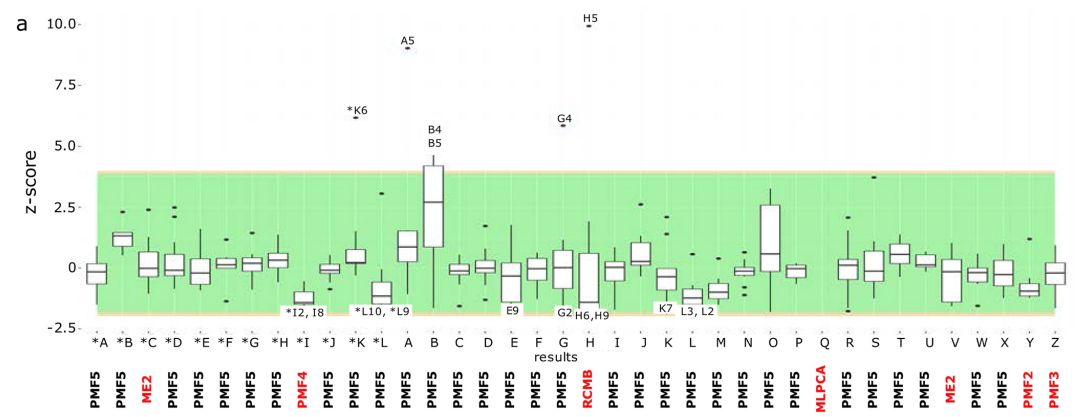
\includegraphics[width=1.0\linewidth]{chapter01/belisEvaluation2020_fig2a.png}
    \caption{Comparabilité des séries temporelles obtenues par les 38 différentes solutions
    sur l'étude de comparaison des modèles sources-récepteurs sur le site de Lens par
    rapport à la moyenne de l'ensemble des différentes études. L'axe X représente chacune des
    solutions des participants, et l'axe Y le z-score, mesure de la similitude des
contributions temporelles. La solution commune IGE-INERIS-EMD est la solution W.\\
Source: \cite{belisEvaluation2020}}%
    \label{fig:chapter01/belisEvaluation2020_fig2a}
\end{figure}

\subsection{Atouts et limitations des différents modèles récepteurs}%
\label{ssub:atouts_et_limitations_des_différents_modèles_récepteurs}

Les 3 types de modèles listés précédemment (CTM, CMB et PMF) ne sont pas les seuls
utilisés, mais représentent néanmoins la très grande majorité des études d'attribution
des sources. Leurs atouts et limitations sont repris dans le
tableau~\ref{tab:comparison_SA} et nous expliquerons dans cette partie plus en avant le
choix pour cette thèse du modèle PMF avec analyse chimique sur filtre.

\begin{table}[!ht]
    \begin{ThreePartTable}
        \centering
        \caption{Forces et limitations des différents modèles d'attribution des sources}
        \label{tab:comparison_SA}
        \footnotesize
        \begin{tabular}{cp{0.43\textwidth}p{0.43\textwidth}}
        \toprule
        Type & Atouts & Limitations \\
        \midrule
        CTM &
        \begin{itemize}[topsep=0pt, left=0pt, label={\unicodesymbols ✔}]
          \item Grande couverture spatiale et temporelle
          \item Comparaison facilité : sources identiques partout\tnote{a}
          \item Prévision à court et long terme
          \item[{\unicodesymbols ~}] Peu de subjectivité\tnote{b}
        \end{itemize}
            &
        \begin{itemize}[topsep=0pt, left=0pt, label={\unicodesymbols ✘}]
          \item Nécessite des cadastres d'émissions
          \item Nécessite un modèle météo
          \item Ne voit que ce qui est donnée des cadastres
          \item Variabilité temporelle des émissions peu robuste
          \item Nombre d'espèces chimiques limités
        \end{itemize}
        \\ \midrule
        CMB & 
        \begin{itemize}[topsep=0pt, left=0pt, label={\unicodesymbols ✔}]
          \item Spécificité du site potentiellement prise en compte
          \item Grand nombre d'espèces pouvant être utilisé
        \end{itemize}
            & 
        \begin{itemize}[topsep=0pt, left=0pt, label={\unicodesymbols ✘}]
          \item Faible représentativité spatiale et temporelle
          \item Prélèvement et analyses couteux (humain et financier)
          \item Profils des sources fixes et connu à l'avance
          \item Nécessite une base de connaissance de profils chimique
          \item Subjectivité de l'expérimentateur
        \end{itemize}
        \\ \midrule
        PMF &
        \begin{itemize}[topsep=0pt, left=0pt, label={\unicodesymbols ✔}]
          \item Pas besoin de connaissance a priori des sources
          \item Spécificités du site prise en compte
        \end{itemize}
            & 
        \begin{itemize}[topsep=0pt, left=0pt, label={\unicodesymbols ✘}]
          \item Faible représentativité spatiale et temporelle
          \item Prélèvement et analyses couteux (humain et financier)
          \item Nécessite des espèces traceuses
          \item Grand nombre d'échantillons requis
          \item Subjectivité de l'expérimentateur
        \end{itemize}
        \\
        PMF-AMS &
        \begin{itemize}[topsep=0pt, left=0pt, label={\unicodesymbols ✔}]
          \item Grande caractérisation de la matière organique
          \item Possibilité de résolution temporelle très fine (mesure on-line)
        \end{itemize}
            & 
        \begin{itemize}[topsep=0pt, left=0pt, label={\unicodesymbols ✘}]
          \item Difficultés d'interprétation
          \item Cible uniquement la matière non réfractaire
          \item Peu utile pour la réglementation
        \end{itemize}
        \\
        PMF-filtre &
        \begin{itemize}[topsep=0pt, left=0pt, label={\unicodesymbols ✔}]
          \item Large gamme de famille d'espèce chimique
          \item Directement applicable pour la régulation
          \item D'autres analyse possible sur le même filtre (potentiel oxydant par
              exemple)
        \end{itemize}
            & 
        % \begin{itemize}[topsep=0pt, left=0pt, label={\unicodesymbols ✘}]
        % \end{itemize}
        \\
        \bottomrule
        \end{tabular}
    \end{ThreePartTable}
\end{table}


\subsubsection{La PMF : modèle théoriquement le moins biaisé par l'information a priori}%
\label{ssub:choix_du_modèle_pmf}

Lorsque l'on s'intéresse à un site particulier, le contexte géographique peut nous donner
des indications sur les sources majoritaires. Seulement, prédéfinir à l'avance les sources
possibles résulte en un biais évident : on ne voit que ce que l'on s'attend à voir.
L'utilisation des CTM ou du CMB ne nous permet donc pas de découvrir de nouvelles sources
locales. Au mieux, le modèle échouera à reproduire les observations, ce qui indiquerait
une source ou un processus manquant.

Au contraire, la PMF étant totalement agnostique aux sources ou processus réels, les
facteurs déterminés reflètent les observations locales sans biais. Ainsi, l'ajout d'une
espèce peut conduire à découvrir et quantifier une nouvelle source d'émission ou processus
atmosphérique, jusqu'alors non prise en compte ou sous-estimée, comme nous le verrons dans
le chapitre~\ref{cha:approfondissement_des_connaissances_des_sources_des_pm}. À noter
également que la réciproque est vraie : la non-prise en compte d'une espèce chimique peut
conduire à ne pas identifier un facteur important, ayant un impact direct sur la
contribution des autres facteurs aux PM.
Toute la difficulté réside dans le choix des ``bonnes espèces'' et en l'interprétation de
ce modèle, fondé sur nos connaissances géochimiques.

\subsubsection{Analyses chimiques ou spectrométrie de masse}%
\label{ssub:analyses_chimiques_ou_spectrometrie_de_masse}

Comme expliqué précédemment, les PM sont composées en grande majorité de matière organique
--tout du moins dans les écosystèmes européens.  Devant la myriade d'espèces chimiques la
constituant, la caractérisation exhaustive de cette matière organique est illusoire.
Pourtant, il est possible de décrire cette matière organique de manière extrêmement
précise par spectrométrie de masse (\textit{aerosol mass spectrometer} (AMS)). On obtient alors des
fragments d'espèces chimiques ionisées, caractérisés par leur ratio masse sur charge ionique
($m/z$ ou Th).

L'avantage principal est la quasi-exhaustivité et la possibilité de
résolution temporelle fine pouvant aller à un échantillon toutes les 2 minutes
\autocite{marmureanuOnline2020}.  Le désavantage majeur est la quantité extrêmement
importante de données générées à analyser. En plus, l'identification des fragments en
facteur PMF est difficilement interprétable en termes de source d'émission. En effet, si
l'on retrouve des facteurs primaires comme l'\textit{hydrocarbon-like organic} (HOA)
pouvant être relié au trafic ou le \textit{biomass burning organic aerosol} (BBOA),
certains, reflétant des processus secondaires, sont plus ``abstraits'' et classés selon leur
degrée d'oxygénation : \textit{less-oxidized oxygenated organic aerosol} (LO-OOA) ou
encore \textit{more-oxidized oxygenated organic aerosol} (MO-OOA).
Enfin, l'utilisation de PMF sur données AMS présente aussi la limitation de ne prendre en
compte que la matière non réfractaire. Il est donc difficile voire impossible d'estimer la
contribution des poussières crustales, présentant très peu ou pas de matière organique. De
même, les émissions secondaires du trafic comme l'usure des freins ou des pneus ne peuvent
pas être retrouvées par PMF-AMS.

Les méthodes de PMF-AMS sont cependant récentes et en développement très rapide et ces
dernières années de nouveaux travaux tentent de combiner mesure AMS et mesures chimiques sur
filtre~\autocite{vlachouAdvanced2018,vlachouDevelopment2019}.  Cependant, lorsque l'on
s'intéresse aux sources d'émissions dans une optique réglementaire et non de compréhension
fine des processus secondaires, la PMF avec analyses chimiques sur filtre reste pour
l'instant davantage adaptée que la PMF-AMS.

En effet, les analyses sur filtres permettent l'identification des types d'espèces
chimiques plus larges qu'uniquement la matière organique (ions et métaux notamment).  Le
recul scientifique des analyses chimiques sur filtres est également appréciable pour
déterminer les sources ou processus à l'œuvre.

Enfin, et plus spécifiquement à cette thèse, nous chercherons à analyser d'autres
variables que la chimie (notamment le potentiel oxydant, voir
section~\ref{sec:le_potentiel_oxydant_des_aerosols}) sur les mêmes échantillons que les
mesures de chimie. Cela exclut donc les données AMS on-line et donc la résolution
temporelle fine, réduisant l'intérêt de cette méthode pour cette thèse.

\subsubsection{Nécessité d'inclure des espèces traceuses dans les PMF}%
\label{ssub:nécessité_d_inclure_des_espèces_traceuses}

L'une des limitations des PMF provient de leur sensibilité aux espèces chimiques
utilisées.

\todo{Discussion espèce organique}
\autocite{srivastavaSpeciation2018a}etc


\todo{
introduire la notion de limitations liées au cout analytique : on sait faire les HULIS sur
les filtre, et on sait que cela représente une espèces importante pour la compréhension
des sources (Srivastava) et potentiellement pour le PO. Mais cette analyse demande bcp de
temps, et on ne peut pas la mesurer sur toutes nos séries
}

\section{Vers une mesure unifiée de l'impact sanitaire : le potentiel oxydant}%
\label{sec:le_potentiel_oxydant_des_aerosols}

Devant la grande variété de chimie, forme, taille, etc. des aérosols, il apparaît
compliqué de résumer la toxicité de l'air que l'on respire à la simple concentration
massique en aérosols. En effet, il est évident que respirer un~\si{\ugm} de sable n'aura
pas le même impact sur notre santé qu'un~\si{\ugm} de mercure ou de plomb.  Seulement, la
mesure des concentrations massiques est l'une des plus simples à implémenter en routine et est également
facilement automatisable, permettant ainsi un premier ordre de grandeur de l'exposition
des populations. Aussi, il est important de rappeler que les aérosols n'ont pas qu'un
impact sanitaire, mais également climatique ou environnemental (voir
section~\ref{ssub:impacts_climatiques} et~\ref{ssub:impacts_environnementaux}),
pour lesquels la mesure de la concentration est tout à fait adaptée.

Bien qu'il ne soit pas encore établi de mécanismes clairs entre les PM et leur impact
sanitaire, leur capacité à induire un stress oxydant dans notre corps est une des
hypothèses privilégiées, notamment par leur transport ou induction d'espèces réactives de
l'oxygène (\textit{reactive oxygen species}
(ROS))~\autocite{squadritoQuinoid2001,liParticulate2003a,liUltrafine2003,gonzalez-flechaOxidant2004}.

La présence de ROS dans nos cellules est un phénomène naturel, produit en grande partie
par catabolisme oxydatif et notamment la respiration cellulaire lors du transfert
d'électron depuis le \ce{O2} vers l'accepteur final \ce{H2O}. Lors de ce transfert, il est
possible d'avoir des électrons captés par d'autres espèces chimiques, conduisant à la
formation de l'anion superoxyde \ce{O2^{.-}} ou \ce{HO^{.-}}, entre autres.
En temps normal, les anti-oxydants cellulaires réduisent ces oxydants avant qu'ils ne
puissent avoir des effets délétères sur les chaînes protéiques ou les acides nucléiques.

Seulement, au contact de nos poumons, les PM, oxydantes, interagissent donc avec nos
anti-oxydants naturels~\autocite{kellyProtein2003}, voir traversent la paroi épithéliale
et entrent dans la circulation générale et les cellules internes, comme illustré
figure~\ref{fig:mecanisme_oxydation}.
Dans un premier temps, les défenses anti-oxydantes sont mobilisées, puis si l'oxydation se
poursuit, on a alors une inflammation, puis cytotoxicité~\autocite{baezaPollution2007}.

\begin{figure}[ht]
    \centering
    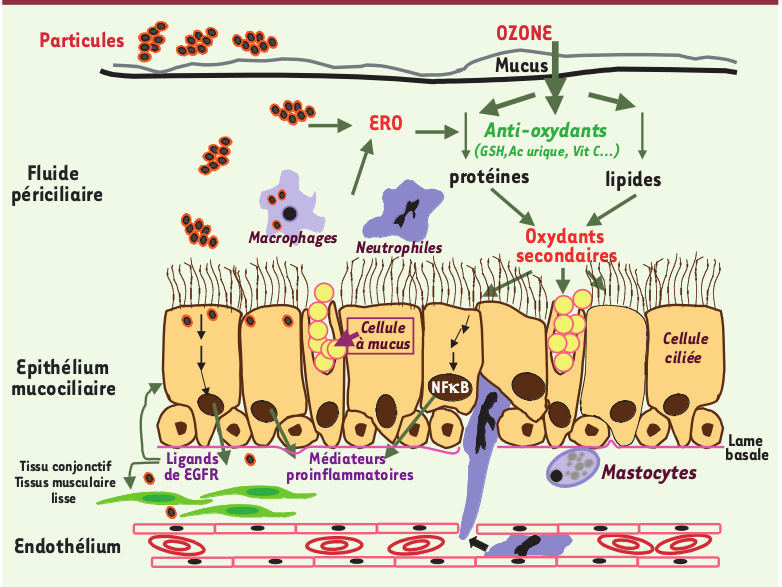
\includegraphics[width=0.8\linewidth]{chapter01/OxydativeMechanism_BaezaMorano2007.png}
    \caption{Mécanismes de toxicité de l’ozone et des particules atmosphériques dans les voies
    aériennes. Crédit : \cite[figure 1]{baezaPollution2007}}%
    \label{fig:mecanisme_oxydation}
\end{figure}

Afin de répondre à cette problématique de métrique sanitaire des PM, il a été proposé
par~\cite{zielinskiModeling1999} et \cite{choRedox2005} une nouvelle mesure, intégratrice
des propriétés physico-chimique des aérosols, sensée être plus proche des impacts
sanitaires occasionnés par les PM : le \textit{potentiel oxydant} (PO, ou
\textit{oxidative potential} (OP)).  Cette nouvelle mesure tente de quantifier les espèces
réactives de l'oxygène présentes ou induites par les aérosols, en utilisant la mise en
contact des aérosols avec un anti-oxydant.  Le suivi de la cinétique de la réaction permet
ainsi d'estimer la réactivité de l'échantillon, prenant en compte non seulement sa chimie,
mais aussi la taille et forme des particules à travers leurs surfaces de réaction et
également les potentiels ``effet cocktail'' lors de la combinaison de différentes espèces
chimiques.

L'avantage de cette méthode acellulaire réside en son faible coût, mais elle aussi est
non-invasive et implémentable en routine en laboratoire, comparativement aux tests
cellulaires nécessitant des prélèvements de tissu et des analyses des protéines marqueuses de
l'inflammation.  Elle permet également une confrontation facilitée aux autres informations
dont l'on dispose sur les PM provenant du même échantillon.

\subsection{Méthodologie de mesure}%
\label{sub:methodologie_de_mesure}

Il n'existe pas à l'heure actuelle de méthodologie standardisée de mesure du potentiel
oxydant. Plusieurs méthodes coexistent et apportent chacune une vision différente du PO.

Il faut noter également que ces méthodes n'ont pas été développées lors de ma thèse mais
s'appuient sur les travaux de \cite{calasPollution2017} et que les échantillons ont été
analysés par les différent·e·s techniciennes et techniciens du plateau analytique
Air-O-Sol de l'IGE.

\subsubsection{Différents agents réactants}%
\label{ssub:differents_agent_reactant}

La mesure du PO se faisant par suivi cinétique de la déplétion d'un anti-oxydant
lorsqu'il est mis au contact des PM, le choix de l'anti-oxydant induit des mesures de PO
différentes. Au cours de cette thèse, 2 mesures différentes sont utilisées conjointement :
le test au dithiothreitol (DTT) et à l'acide ascorbique ou vitamine-A (AA), et sont
explicités dans le chapitre suivant (section~\ref{sub:potentiels_oxydants}).

D'autres méthodes de mesures du PO existent, mais n'ont pas été utilisées au courant de
cette thèse, à savoir :
\begin{description}
    \item[Electron spin résonance ESR] sensé ciblé particulièrement le radical
        \ce{HO^{.}} \autocite{shiHydroxyl2003,shiTemporal2003}
    \item[DCFH]\todo{ref}
    \item[Mélange d'anti-oxydant] Bien que la plupart du temps testé indépendamment, il est
        possible d'estimer un ``PO moyen'' par la mise en contact de différents
        anti-oxydants simultanément (acide ascorbique, glutation et urée par exemple)~\autocite{calasComparison2018}
    \item[todo] \todo{Mesure directe de OH° (mise en place en à l'IGE dans le cadre d'un
        programme financé par le LEFE-CHAT)}
\end{description}

\subsubsection{Un ``meilleur'' test que les autres ?}%
\label{ssub:un_meilleur_test_que_les_autres_}

Les différents tests de PO ne sont pas sensibles aux mêmes espèces chimiques ni même aux même
conditions physico-chimiques. En effet, l'étude de \cite{kunzliComparison2006} sur 20
sites européens présente des corrélations différentes entre le PO mesuré par ESR, AA ou
GSH au regard de la masse des PM et les métaux les constituants.
Ce résultat a été retrouvé depuis par de nombreuses études, et pour le test au DTT et DCFH
également. Par conséquent, cela montre que différents constituants des PM agissent
différemment et à travers des mécanismes oxydatifs divers, capturés par certains tests et
non par d'autres.
Il est donc probable que certaines affections sanitaires soient reliées à un test donné, et
d'autres affections à un autre test. En l'absence de travaux plus approfondis en toxicologie
et épidémiologie, il n'est donc pas possible en l'état actuel des connaissances de trancher
pour ``le meilleur test de PO''.

Par conséquent, les travaux de cette thèse s'emploient à étudier conjointement le PO
mesuré par DTT et par acide ascorbique.


\subsection{Attribution du PO aux sources d'émissions des PM}%
\label{sub:attribution_du_po_aux_sources_d_émissions_des_pm}

Les mesures de PO étant fastidieuses, il a fallu attendre la mise en place de technique
de semi-automatisation pour obtenir des séries temporelles de mesure de ``longue durée''. Les récents
travaux de \cite{fangSemiautomated2015}, parallèlement aux travaux de
\cite{calasPollution2017}, ont permis ce pas technique, permettant l'analyse accrue de
prélèvements et les premières séries annuelles de mesure des PO, conjointement avec
l'analyse de la chimie des filtres prélevés.

\subsubsection{Corrélation PO -- chimie}%
\label{ssub:corrélation_po_chimie}

Les liens entre la chimie des particules et les résultats de PO s'est dans un premier temps focalisé
sur la simple corrélation univariée. Ainsi, le Cu présente de fortes corrélations
avec le \PODTT{} et \POAA, de même que le carbone organique, etc. Seulement, la simple
corrélation montre également une forte corrélation entre le \PODTT{} et le \ce{NO3-},
pourtant inerte en termes d'oxydo-réduction.
En effet, une corrélation n'implique pas une causalité, et cette corrélation ne résulte
que d'une co-correlation entre le \ce{NO3-} et d'autres espèces, rédox-actives.

\todo{parler des quinones, add ref, etc}


\subsubsection{Sources de PM et de PO}%
\label{ssub:sources_de_pm_et_de_po}

% Enfin, il n'est pas possible de mesurer l'ensemble des espèces chimiques constituant les
% PM. Devant cette foultitude, il paraît donc illusoire de pouvoir attribuer un PO
% intrinsèque à chacune des espèces chimique.
% En revanche, si l'on bénéficie d'un nombre suffisant d'échantillon, il est alors possible
% d'estimer les sources ou facteurs d'émissions (voir
% section~\ref{sec:source_apportionment_of_pm}). Ce faisant, la vision par ``source'' plutôt
% que par ``espèce'' permet une agrégation de l'information, en regroupant un ensemble
% d'espèce, mesurée ou non, provenant d'une même source d'émission, en une seule variable.
% Ainsi, il est possible d'attribuer un PO à une source donnée, sans pour autant avoir
% besoin de savoir quelles sont les espèces chimiques émises par cette source qui
% contribuent au PO.
% De plus, en termes de régulation, la vision par source est davantage pertinente car permet
% potentiellement une action politique plus rapide que s'il s'agissait de cibler une espèce
% chimique particulière.

Il est aussi possible de chercher à attribuer un PO non pas à une espèce chimique mais à
une source spécifique.
\todo{work in progress}

\paragraph{Mesures directes à l'émission}%
\label{par:mesures_directes_à_l_émission}

\todo{parler de l'étude de Lucille dans sa thèse. Citer un projet possible avec l'INERIS,
en cours d'écriture. }

\paragraph{Études sur sites et en air ambiant}%
\label{par:études_sur_sites_et_en_air_ambiant}

Les premières études de ce type sont celles de
\cite{vermaReactive2014,batesReactive2015,fangOxidative2016}, et utilisent 2 approches
différentes :
\begin{enumerate}
    \item Incorporation de PO comme variable d'entrée d'une étude PMF au même titre qu'une
        autre espèce chimique ;
    \item Analyse de sources via le CMB (sans PO), puis régression linéaire entre les
        sources de PM ainsi déduites et le PO.
\end{enumerate}
Bien que de façon inhérente aux différences entre PMF et CMB les sources retrouvées ne
sont pas exactement les mêmes, les auteurs montrent que la combustion de biomasse est la source
principale de \PODTTv, suivie de près par le trafic routier (ensemble des émissions
véhiculaires et de la remise en suspension de poussière de route), puis le sulfate
d'ammonium et enfin un facteur de composés organiques secondaires solubles.
Concernant le \POAAv, \cite{fangOxidative2016} (voir
figure~\ref{fig:chapter01/fangOxidative2016-fig4}) estiment à autour de \SI{45}{\percent} la
contribution des émissions véhiculaires et à environ \SI{50}{\percent} la contribution de
facteur secondaire (organique et inorganique).

\begin{figure}[ht]
    \centering
    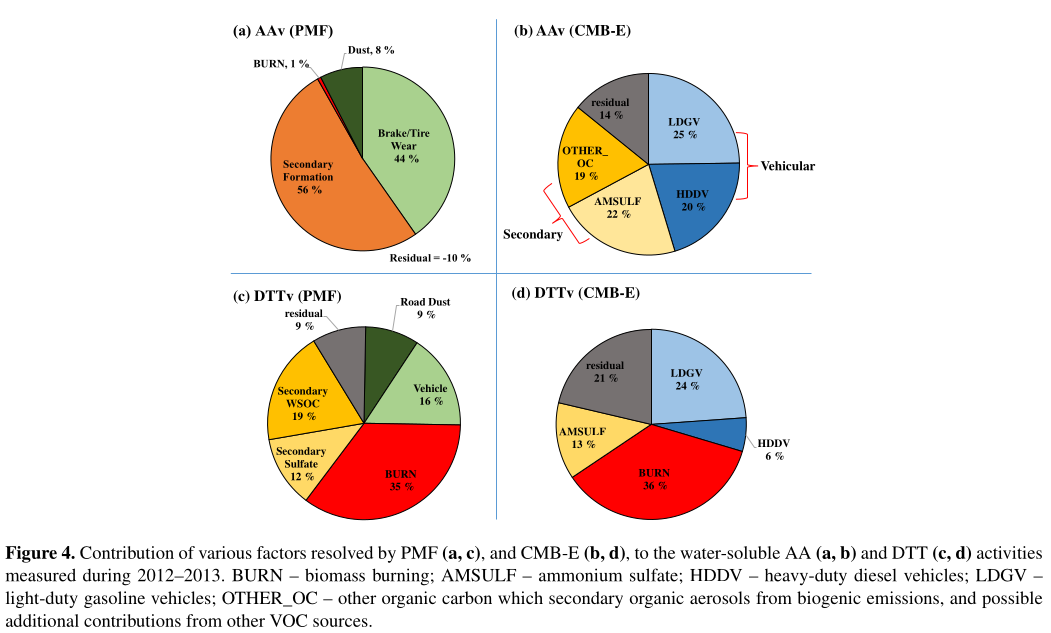
\includegraphics[width=1.0\linewidth]{chapter01/fangOxidative2016-fig4.png}
    \caption{Contribution des sources de PM aux \POAAv{} et \PODTTv{} par l'étude de
    \cite{fangOxidative2016} portant sur un ensemble de 238 échantillons sur 3 sites
        distincts à Atlanta, US, pendant l'année 2012-2013.}%
    \label{fig:chapter01/fangOxidative2016-fig4}
\end{figure}

Lors du commencement de ma thèse, seules ces études étaient, à ma connaissance,
disponibles dans la littérature concernant l'attribution des sources de PM aux potentiels
oxydants.  Depuis, de nouvelles études ont été publiées, et seront discutées dans le
chapitre~\ref{cha:estimation_des_sources_de_PO}.


\section{Objectifs de cette thèse}%
\label{sec:positionnement_de_cette_thèse}

Ma thèse s'inscrit donc dans cette double problématique de l'identification et de la
quantification des contributions massiques des différentes sources d'émission de PM en air
extérieur, mais aussi de leurs contributions au nouvel indicateur qu'est le potentiel
oxydant.

Premièrement, il s'agit d'améliorer l'outil de déconvolution des sources de PM
\textit{Positive Matrix Factorization}, non pas par de nouveaux développements mathématiques de
résolution de l'équation de conservation des masses, mais par l'élaboration d'une
expertise dans les différentes paramétrisations de ce modèle, dans son entraînement et
dans la critique de ses résultats. Notamment, la question de la présence de l'ensemble
des sources majoritaires se posera dans le
chapitre~\ref{cha:approfondissement_des_connaissances_des_sources_des_pm}, à travers
l'implémentation de nouveaux traceurs chimiques ou isotopiques.
Également, les incertitudes des solutions PMF ne sont quasiment jamais explicitées alors
que c'est une question centrale qui intéressent d'autant plus les décideurs publics. Mes
travaux tenteront donc de quantifier les incertitudes des contributions des sources aux
espèces mesurées.
Aussi, pour pouvoir généraliser des études PMF à différents sites, il faut auparavant
non seulement s'assurer que les méthodes sont similaires entre les études (mêmes espèces
chimiques…) mais aussi estimer objectivement la similitude de deux facteurs que l'on estime provenir
de la même source d'émission, c'est-à-dire comparer les solutions entre elles.

\todo{Blabla PO}

\subsection{Questionnement et plan de la thèse}%
\label{sub:plan_de_la_thèse}

Ainsi, mes recherches tenteront de répondre aux questions suivantes :

\begin{itemize}
    \item Comment obtenir des contributions et profils de sources reflétant au mieux les
        processus d'émissions et de transformation dans l'atmosphère ?
        (Chapitre~\ref{cha:approfondissement_des_connaissances_des_sources_des_pm})
    \item Est-il possible de diminuer la subjectivité de l'expérimentateur dans ces
        études d'attribution des sources ?
        (Chapitre~\ref{cha:approfondissement_des_connaissances_des_sources_des_pm})
    \item Comment comparer efficacement 2 profils attribués à la même source, à
        différents sites de prélèvement et différentes années de mesure ?
        (Chapitre~\ref{cha:approfondissement_des_connaissances_des_sources_des_pm})
    \item Comment remonter à la contribution des sources de PO une fois les sources
        d'émissions de PM identifiées ?
        (Chapitre~\ref{cha:estimation_des_sources_de_PO})
    \item Les sources contribuants au potentiel oxydant sont-elles les mêmes que celles
        contribuant à la masse des PM ?
        (Chapitre~\ref{cha:estimation_des_sources_de_PO})
    \item Est-ce que les valeurs PO des sources des PM sont les mêmes à large échelle spatiale ou
        sont-elles dépendantes du lieu considéré ?
        (Chapitre~\ref{cha:estimation_des_sources_de_PO})
    \item Est-il possible, à terme, d'obtenir une prévision du PO intégré à la prévision
        de la qualité de l'air, complémentairement à la concentration massique ?
        (Chapitre~\ref{cha:estimation_des_sources_de_PO} et~\ref{cha:travaux_futur})
\end{itemize}

Ces différentes questions seront abordées entre autres avec la présentation des résultats de
recherches déjà publiés dans 7 articles scientifiques auxquels j'ai contribué (dont 2 
en premier auteur) ainsi que par des travaux en cours de publication (6, dont 2 en premier auteur).
La liste complète de ces travaux est fournie en annexe~\ref{annexe:CV} et s'appuie sur un
grand nombre de programmes de recherche
(voir~\ref{annexe:programmes_ayant_financés_la_thèses}). Les articles en
premier auteur sont reproduits in extenso.

% \clearpage
% \printbibliography[segment=\therefsegment,heading=subbibliography]
%
% \chapter{Matériel et méthode}
% \label{cha:materiel_et_methode}
% \PartialToc
% \clearpage
% 
\section{Stratégie de cette thèse (et du groupe CHIANTI)}%
\label{sec:stratégie__du_groupe_chianti}

\subsection{Place de ma thèse dans les problématiques de CHIANTI}%
\label{sub:place_de_ma_thèse_dans_les_problématiques_de_chianti}

Le groupe de recherche de chimie atmosphérique, neige, transfert et impacts (CHIANTI) au
sein duquel j'ai effectué ma thèse à l'IGE s'emploie ``à identifier les sources, les puits et
mécanismes de transformations des espèces chimiques générées par les activités humaines
(en particulier) afin de déterminer leur impact sur le climat, la composition et la
qualité de l’air, et les écosystèmes
enneigés''\footnote{\url{http://www.ige-grenoble.fr/-Chimie-atmospherique-CHIANTI-}}.
Le cadre de ma thèse concerne donc une sous partie de ces recherches, portant sur l'étude
de la qualité de l'air.

Une partie des travaux concerne un aspect fondamental de compréhension des processus
conduisant à la présence d'aérosols dans l'atmosphère, étudié par le biais de prélèvements sur le
terrain et d'analyses sur filtre effectuées par le plateau analytique Air-O-Sol à travers notamment
l'analyse de la fraction organique des PM (voir
section~\ref{sec:methodologie_de_prélèvement_et_d_analyse}).
Les mesures enregistrées dans la ``filtrothèque'' portent actuellement sur \num{18000}
filtres répartis sur plus de 80 sites différents et ont été possibles grâce à de très nombreux partenariats.

Ces partenariats avec les AASQUA ou d'autres instituts (LCSQA, INERIS, ADEME, ANSES...),
constituent également un volet important des recherches portant sur la réglementation et sur
la connaissance des processus et la quantification des sources d'émissions conduisant aux
concentrations de PM en air ambiant.
Différents programmes de recherche ont ainsi été élaborés en vue d'une amélioration de la
qualité de l'air (grâce au programme PRIMEQUAL par exemple) en appui à des plans de protections de
l'atmosphère (PPA). À titre d'exemple, l'importance
de la combustion de biomasse domestique en vallée alpine a pu être démontrée, conduisant
entre autres à la mise en place de la prime Air-bois, incitatif au remplacement des vieux
poêles à bois. Les conséquences de cette action ont été suivies et
analysées au sein du laboratoire depuis plusieurs années maintenant, avec le programme DECOMBIO~\autocite{chevrierDECOMBIOContribution2016,chevrierChauffage2016,allardQualite2018}.
Une liste des programmes ayant directement conduit aux données présentées dans cette thèse
est proposée en annexe~\ref{annexe:programmes_ayant_financés_la_thèses}.

Finalement, nous essayons aussi de nous rapprocher de l'impact sanitaire des PM à
travers le développement de méthodes d'analyse du potentiel oxydant (PO ou \textit{oxidative potential OP}) (voir
section~\ref{sub:potentiels_oxydants}). En plus du développement méthodologique de leurs
mesures, ces efforts du groupe ont porté sur l'analyse des PO sur plus de 45 sites de prélèvement différents, pour un
total de plus de 6500 échantillons pour lesquels le PO a été mesuré.
L'avantage majeur de la mesure du PO sur filtre consiste en la concomitance des mesures de
PO et de chimie, permettant des recherches couplées sur la chimie de l'aérosol et de son
potentiel oxydant, afin à terme de mieux comprendre la variabilité des différentes
mesures de quantification du PO et leurs liens avec d'autres variables métrologiques (par
exemple les connexions avec les déterminants géochimiques). Parallèlement, la pertinence de la
mesure du PO comme métrique sanitaire et sa comparaison avec la variable
réglementaire en vigueur (la concentration des PM) n'est pas encore totalement établie.
Les travaux du groupe sont donc également focalisés sur ce point, notamment par des travaux
pluridisciplinaires associant géochimistes et épidémiologistes.

\subsection{Méthodologie générale}%
\label{sub:méthodologie_general}

Ma thèse s'inscrit en plein cœur de ces thématiques du groupe de recherche et est transverse aux
différentes thématiques abordées, à savoir la détermination des sources d'émission d'intérêt
sanitaire.

Pour ce faire, la méthodologie générale suivante est donc adoptée et résumée sur le schéma
synthétique~\ref{fig:chapter01/workflow} :

\begin{enumerate}
    \item Grâce aux mesures de chimie et au modèle PMF, il s'agit de retrouver au mieux les
        sources d'émissions de PM;
    \item On entreprend ensuite de coupler les données issues de la PMF et les mesures de PO pour construire un
        modèle d'inversion permettant l'estimation de la contribution des différentes
        sources aux mesures des potentiels oxydants ;
    \item Ces résultats permettent ensuite de tenter d'estimer la variabilité géographique du potentiel oxydant des sources de PM.
\end{enumerate}

Chacun de ces items sera abordé dans des chapitres dédiés.

\begin{figure}[ht]
    \centering
    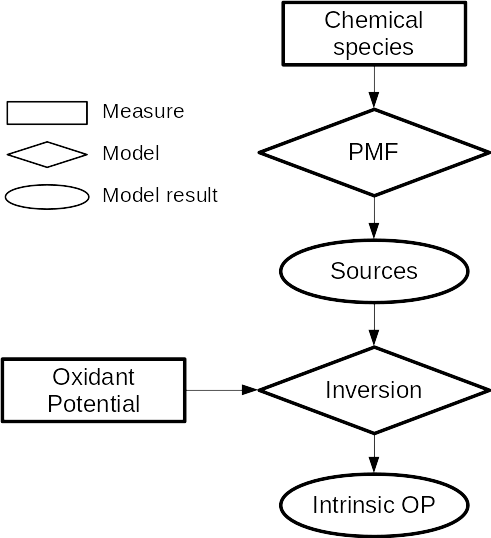
\includegraphics[width=0.5\linewidth]{chapter01/workflow.png}
    \caption{Méthodologie générale suivie au cours de cette thèse.}%
    \label{fig:chapter01/workflow}
\end{figure}


\subsubsection{Choix du modèle d'attribution de source}%
\label{ssub:choix_du_modèle_d_attribution_de_source}

Le choix du modèle source-récepteur PMF est motivé par son aptitude à reproduire les
concentrations locales sans préjuger a priori des spécificités du site de prélèvement. La
capacité du ME-2 à introduire des contraintes géochimiques est également un atout
important justifiant l'usage du modèle PMF.
Enfin, les précédents travaux au sein de l'équipe CHIANTI, en particulier ceux d'Antoine Waked, Benjamin Golly,
Florie Chevrier et Dalia Salameh sur le modèle PMF représentent également une expertise
appréciable justifiant le choix de cette méthode.

\subsubsection{Échantillons et analyses}%
\label{ssub:échantillons_et_analyses}

Les prélèvements, les mesures de concentrations des différentes espèces chimiques et les
mesures du PO s'appuieront sur les travaux préalables et en cours de l'équipe CHIANTI et
particulièrement ceux effectués sur le plateau analytique Air-O-Sol.
La base de données accumulées depuis plusieurs années est en construction permanente et mon travail sur son organisation est brièvement décrit ci dessous.

\subsubsection{PO et chimie ou PO et sources ?}%
\label{ssub:chimie_ou_sources_}

Le choix a été fait de ne pas utiliser directement les espèces chimiques comme prédicteur
des PO. En effet, sur la myriade d'espèces chimiques présentes sur les aérosols, seule une
partie infime est effectivement mesurée. Il n'est donc pas possible d'avoir une vue
exhaustive de la chimie des PM et l'attribution d'un PO intrinsèque par espèce chimique
présenterait nécessairement des biais du fait de corrélations entre une espèce mesurée mais
non redox-active (par ex. le lévoglucosan) et des espèces co-émises mais non mesurées (par ex. les
quinones). Quand bien même toutes les espèces seraient mesurées, on se retrouverait alors
avec un système d'équations avec beaucoup trop d'inconnues par rapport au nombre
d'observations (i.e jours de prélèvement), rendant caduque sa résolution.
A contrario, les facteurs PMF agrègent toute cette chimie en quelques variables, tout en
n'ayant besoin que de quelques espèces traceuses des émissions ou processus. Par exemple,
la combustion de biomasse est déterminée à partir de la présence de lévoglucosan. On pourra
donc attribuer un PO à la source \textit{combustion de biomasse}, avec concentration en PM
connue et un profil chimique déterminé (et partiellement inconnue), tout en ne sachant
pas exactement quelles espèces chimiques de cette source sont responsables de son PO.



\section{Methodologie de prélèvement et d'analyse}%
\label{sec:methodologie_de_prélèvement_et_d_analyse}


\subsection{Un filtre pour les gouverner tous}%
\label{sub:un_filtre_pour_les_gouverner_tous}

Les données utilisées pour cette thèse proviennent d'analyses faites en laboratoire à
partir de prélèvement de terrain (mesure \textit{off-line}) via des préleveurs
automatiques haut-volume, selon les recommandations de
l'EN~16450:2017~\autocite{cenAmbient2017a}, chaque prélèvement correspondant à une
journée d'échantillonnage. 

L'entiéreté des analyses des différents composés chimiques et de PO se fera sur ce même
filtre, dont différents morceaux seront prélevés, comme le montre la
figure~\ref{fig:chapter02/filter_speciation_en}.

\begin{figure}[ht]
    \centering
    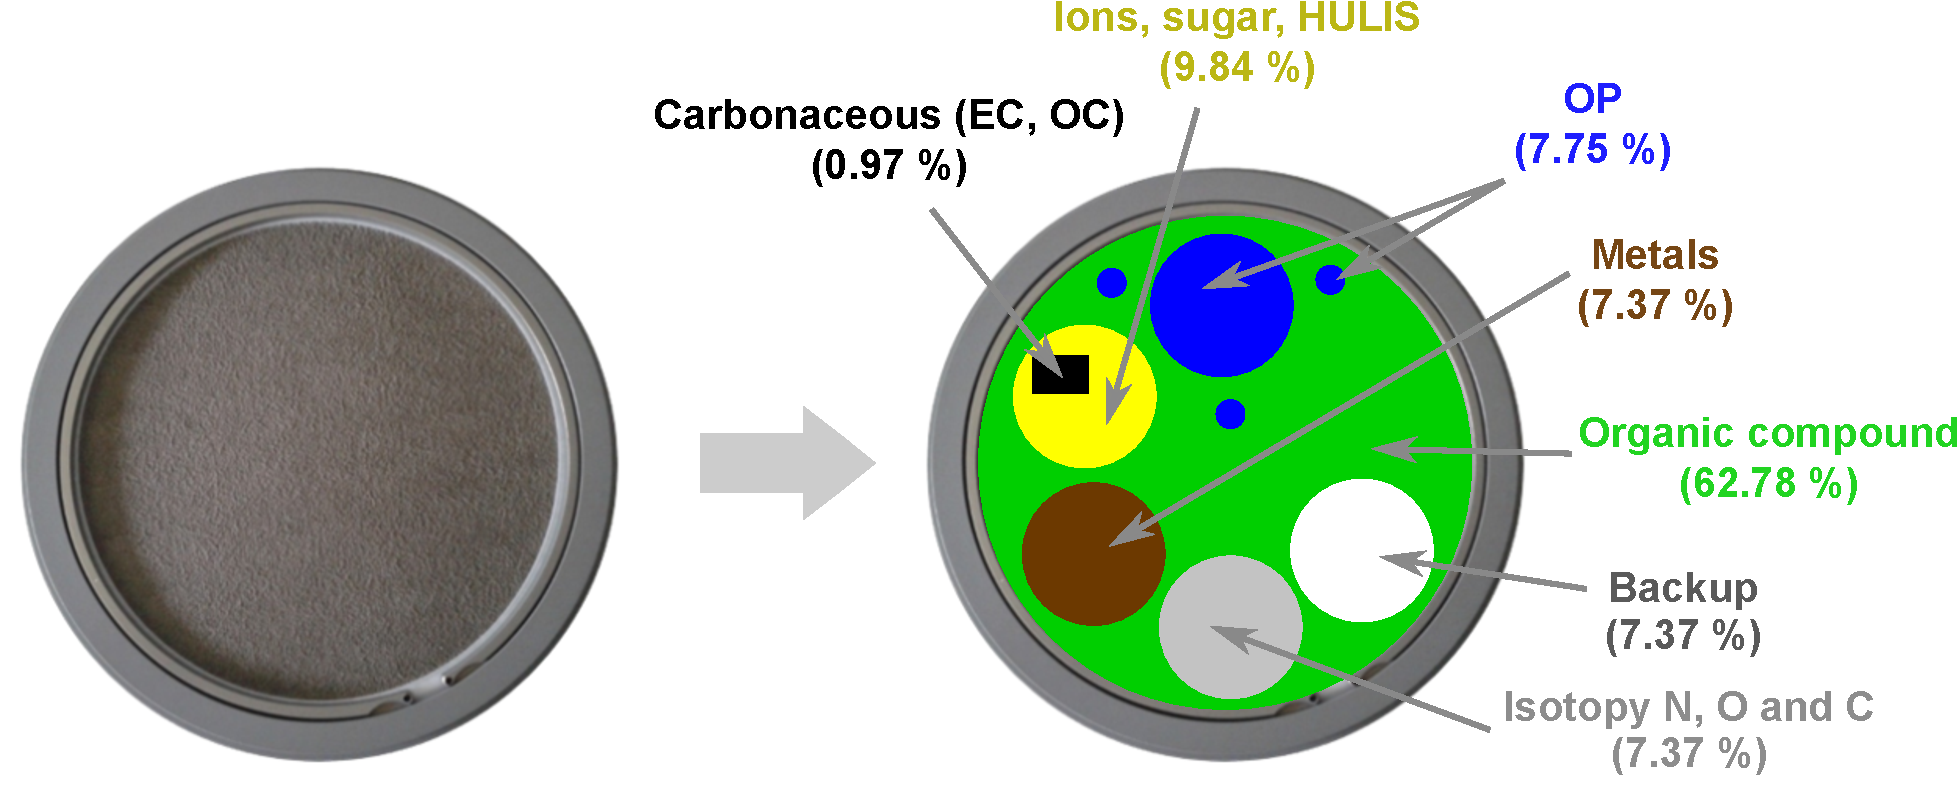
\includegraphics[width=1.0\linewidth]{chapter02/filter_speciation_en.pdf}
    \caption{Séparation typique des différentes surfaces de filtre pour préparation et
    analyses conduites à l'IGE ou dans les laboratoires collaborateurs.}%
    \label{fig:chapter02/filter_speciation_en}
\end{figure}

\subsection{Mesure des composés chimiques}%
\label{sub:analyses_des_composés}

\subsubsection{Préparation des filtres}%
\label{sub:préparation_des_filtres}

Les prélèvements sont réalisés sur des filtres en fibre de quartz pré-chauffés à
\SI{500}{\degreeCelsius} pendant 8 heures pour se prémunir de la présence en espèces
ioniques et organiques. Ces filtres sont chargés dans les porte-filtres des préleveurs
haut-débit (\SI{30}{\cubic\m\per\hour}) DA80 Digitel.

La fraction prélevée correspond très généralement aux \PMdix{} mais certains programmes
ont aussi considéré les \PMdc.
Les analyses réalisées sur ces filtres sont présentées brièvement ci dessous.

\subsubsection{Matière carbonée (EC et OC) : méthode thermo-optique}%
\label{ssub:matière_carbonnée_ec_et_oc_}

L’analyse de la matière carbonée (carbone organique (OC) et carbone élémentaire (EC)) est
réalisée directement sur un poinçon issu du filtre, à l’aide d’un analyseur
thermo-optique~\autocite[Sunset Lab. Analyser]{birchElemental1996}, par le protocole
EUSAAR-2~\autocite{cavalliStandardised2010,cenAmbient2017a}

Le principe de mesure est basé sur la détection par détecteur FID du \ce{CH4} issu de la
combustion puis réduction de la fraction carbonée présente dans l’échantillon. Une
fraction d'échantillon (1 ou \SI{1.5}{\centi\m\squared}) est placée dans un four en quartz
et soumise à différents plateaux de températures et sous des atmosphères plus ou moins
oxydantes. Une calibration journalière est effectuée. L’IGE participe annuellement à des
exercices d’intercomparaison dans le cadre du programme européen ACTRIS.

\subsubsection{Espèces ioniques : chromatographie ionique}%
\label{ssub:espèces_ioniques_par_chromatographie}

L'analyse de la fraction ionique des aérosols et des acides organiques légers est réalisée
sur la phase aqueuse (après extraction du filtre) par chromatographie
ionique~\autocite{jaffrezoSeasonal2005,cenAmbient2017b} (modèle Dionex ICS 3000) avec une
colonne
CS16 pour l’analyse des cations et colonne AS11 HC pour l’analyse des anions. L’analyse
des anions permet la quantification des ions chlorure \ce{Cl-}, nitrate \ce{NO3-} et
sulfate \ce{SO4^2-}. L’analyse des cations permet la quantification du sodium \ce{Na+}, de
l'ammonium \ce{NH4+}, du potassium \ce{K+}, du magnésium \ce{Mg^2+} et du calcium
\ce{Ca^2+}. 
Les concentrations en oxalate et en acide méthane sulfonique (MSA) sont aussi accessibles.
La calibration est réalisée tous les jours à partir de solutions standards certifiées.

\subsubsection{Sucres et autres polyols : HPLC-PAD}%
\label{ssub:sucres_et_autres_polyols_hplc-pad}

L’analyse de la fraction soluble des sucres et des polyols est réalisée sur la phase
aqueuse, par une méthode HPLC avec détection par PAD (Pulsed Amperometric Detection)
(modèle Thermo 5000+) avec des colonnes Metrosep (Carb 1 – Guard+A Supp 15 – 150+Carb
1 – 150)~\autocite{piotQuantification2012,wakedSource2014}.
Cette analyse permet la quantification des saccharides anhydrides (lévoglucosan,
mannosan, galactosan) et des polyols (xylitol, arabitol, sorbitol, mannitol) et sucres
(glucose). La calibration est réalisée tous les jours à partir de solutions standards.
L’IGE a participé dernièrement à une intercomparaison européenne des mesures de
lévoglucosan.

\subsubsection{Cellulose : digestion enzymatique et HPLC-PAD}%
\label{ssub:cellulose_}

La cellulose est mesurée par un protocol améliorant celui de \cite{kunitEnzymatic1996}.
La cellulose est extraite en solution aqueuse, puis l'extraction est faite dans
différentes solutions ensymatique afin de digèrer la cellulose en glucose. Le glucose est
ensuite mesuré par HPLC-PAD.

Brievement, un poiçon de \SI{21}{\mm} de diamètre est extrait du filtre dans un bain à
ultra-son pendant \SI{40}{\minute} dans une solution aqueuse de \SI{3}{\ml} tamponé à pH
4.8 par un buffer au thymol. Deux solutions enzymatiques (cellulase (Sigma Aldrich, C2730)
avec \SI{20}{\ul} de solution aqueuse à \SI{70}{unit.\g^{-1}} et glucosidase (Sigma
Aldrich, 49291), avec \SI{60}{\micro\L} de solution aqueuse à \SI{5}{unit.\g^{-1}}) sont
ajoutées. La solution est incubée à \SI{50}{\degreeCelsius} pendant \SI{24}{h} pour
hydrolyse. L'hydrolyse est arrếtée par chauffage au four à \SI{100}{\degreeCelsius}
pendant \SI{45}{min}. La solution est ensuite centrifugée (\SI{7000}{rpm}) pendant
\SI{15}{min} et extraite par seringue pour analyse en HPLC-PAD.

L' HPLC-PAD (Dionex DX500) est équipée d'une colonne Methrom (\SI{250}{mm} de long,
\SI{4}{mm} de diamètre) par un run isocratique de \SI{40}{min} avec les éluants 
A (50\M 18 nM NaOH), B (\SI{25}{\percent}, \SI{100}{nM} \ce{NaOH} + \SI{150}{nM}
\ce{NaAc}) et C (\SI{25}{\percent}, \SI{220}{nM} \ce{NaOH}). La température de la colonne
est maintenue à \SI{30}{\degreeCelsius}. Le débit d'éluant est fixe à
\SI{1}{\ml\per\minute} et le volume d'injection de \SI{250}{\ul}.
À chaque lot d'analyse est également inclus une solution standard de glucose et de
cellulose (perles de \SI{20}{\um}, Sigma Aldrich, S3504) analysées selon le même
procédé que les échantillons afin de déterminer l'efficacité spécitique de la conversion
enzymatique cellulose-glucose. Le calcul de la concentration finale de cellulose libre
prend en compte ce ratio de conversion, variant entre les lots entre
\SIrange{65}{80}{\percent}.
À cette concentration est soustraite la concentration initiale en glucose, mesurée
parallèlement par HPLC-PAD (décrite section~\ref{ssub:sucres_et_autres_polyols_hplc-pad}).
Enfin, la mesure des blancs de terrains et de laboratoire sont également pris en compte
dans cette mesure.

\subsubsection{Acides organiques légers : HPLC-MS}%
\label{ssub:acides_organiques_légers_hplc_ms}

L’analyse de la fraction soluble d’une vingtaine d’acides organiques légers (C2 – C7) est
réalisée sur la phase aqueuse, par une méthode HPLC avec détection par Spectrométrie de
Masse (Dionex DX500 + MS LCQ Fleet Thermo) avec séparation sur une colonne Waters
Carotenoid. Cette analyse permet la quantification d’une assez large série d'acides
organiques (depuis l’oxalate jusqu’à l’acide benzoïque). Ces acides sont issus de
processus d’oxydation de matière organique d’origine biogénique ou anthropique. La
calibration est réalisée tous les jours à partir de solutions standards.

% Analyses des HULIS par TOC
% L’analyses de la fraction soluble dans l’eau des HULIS (Humic-Like Substances ;
% composés macromoléculaires polyfonctionnels polyacides) est réalisée par une séparation
% avec filtration sur résine DEAE, permettant de ne retenir que les HULIS de
% caractéristiques précises, tout en éliminant les autres espèces solubles de la matière
% carbonée. Ces HULIS sont ensuite élués de cette résine, l’échantillon récupéré étant
% ensuite analysé pour son contenu en carbone total avec un analyseur Shimadzu TOC 5000.
% Les protocoles détaillés ont été mis au point dans le cadre de la thèse de C Baduel (cf
% Hal CNRS).

% Préparation et analyses de traceurs organiques par GC-MS :
% Ces analyses sont réalisées au LCME (Chambéry). Pour réaliser la spéciation
% moléculaire, une fraction de filtre est extraite par extraction solide/liquide
% filtre/solvants organiques (acétone/dichlorométhane 1:1) à 100°C et 100 bar à l’aide
% d’un Accelerated Solvent Extractor (ASE 200 – Dionex). L’extrait est ensuite concentré
% grâce à un évaporateur (TurboVap II – Zimark) puis filtré à 0,1 µm (Anotop 10 –
% Whatman), Cet extrait est ensuite divisé en fractions pour l’analyse de 15 HAP, de
% composés polaires (entre autres de nombreux dérivés de la combustion de la biomasse,
% etc), et de composés apolaires (alcanes C11 à C40 et 10 hopanes), soit environ une
% grosse centaine d’espèces organiques.

% L’analyse des deux dernières séries de composés est réalisée par GC-MS (chromatographie
% gazeuse couplée à un spectromètre de masse ; GC Clarus 500 associée à un MS 560 –
% Perkin Elmer). Pour les composés polaires, avant l’analyse par GC-MS, l’extrait est
% dérivé par ajout du NO-Bis(trimethylsilyl)trifluoroacetamide (BSTFA) + 1% de
% trimethylchlorosilane (TMCS) en proportion 1:1 v/v et sous agitateur chauffant à 50°C
% pendant deux heures. La quantification est réalisée sur des fragments caractéristiques, la
% calibration étant réalisée à partir de solutions standards et de la méthode à l’étalon
% interne deutéré (n-dodecane d26 pour les composés apolaires et levoglucosan d7 pour les
% composés polaires). La bibliothèque de spectre utilisée est la NIST 2001.

% Analyses des HAP :
% L’analyse des HAP est réalisée par HPLC-fluorescence (chromatographie liquide couplée à
% un détecteur par fluorescence ; HPLC de type Series 200 couplée à un détecteur de type
% Series 200a – Perkin Elmer). La colonne de séparation est une colonne de type phase
% inverse C18 (NUCLEOSIL 100-5 C18 PAH, 25cm × 4,6 cm) éluée avec une phase mobile formée
% d’un mélange méthanol/eau en mode gradient. Cette méthode permet l’analyse des 13 HAP
% classés prioritaires par l’US-EPA (Phénanthrène, Anthracène, Fluoranthène, Pyrène,
% Benzo[a]anthracène, Chrysène, Benzo[e]pyrène, Benzo[b]fluoranthène,
% Benzo[k]fluoranthène, Benzo[a]pyrène, Benzo[ghi]pérylène, Dibenzo[a,h]anthracène,
% Indéno[1,2,3-cd]pyrène) ainsi que du rétène et du coronène. Le LCME a participé aux
% dernères intercomparaisons mises en place par le LCSQA.

\subsubsection{Métaux et traces : IPC-MS ou AES}%
\label{ssub:métaux_et_traces}

Les analyses sont réalisées dans un laboratoire qui
participe aux exercices d’intercomparaison organisés par les Mines de Douai. Ces analyses
sont réalisées par ICP-MS après digestion acide (ou ICP-AES selon les sites
d'études)~\autocite{allemanPM102010,mbengueSizedistributed2014,cenAmbient2005}.
Les métaux et éléments traces analysés sont compris dans la liste suivante : Al, Ag, As,
Ba, Be, Br, Bi, Ca, Cd, Ce, Co, Cr, Cs, Cu, Fe, K, La, Li, Mg, Mn, Mo, Na, Ni, Pb, Pd, Pt,
Rb, Sb, Sc, Se, Sn, Sr, Ti, V, Zn et Zr.

\subsection{Mesure des potentiels oxydants}%
\label{sub:potentiels_oxydants}

Le PO acellulaire des aérosols est déterminé par la capacité intrinsèque des particules
atmosphériques à oxyder le milieu pulmonaire en générant/induisant la formation de ROS.
Les différents filtres seront soumis à deux tests de PO complémentaires, choisis pour
leur représentativité (dénommés PO DTT, et PO AA en fonction du substitut de
l’antioxydant pulmonaire impliqué dans le test, le Dithiotréitol (DTT) et l’acide
ascorbique (AA)). 

Pour chacun des deux tests présentés ci-après, des triplicats de mesures sont effectués, un
témoin positif à la 1,4-naphtoquinone est utilisé et les blancs de laboratoire sont
soustraits aux échantillons.

\subsubsection{Prendre en compte la bioaccessibilité: SLF}%
\label{sub:prendre_en_compte_la_bioaccessibilite_slf}

Étant donné que l'on cherche à reproduire le comportement des PM en milieu biologique
(les poumons), il est important de procéder à l'extraction et l'analyse du PO dans un
fluide reproduissant au plus fidèlement possible ce milieu, et non directement dans de
l'eau milli-Q.

Il existe différents types de fluides mimiant les surfactants pulmonaires
(\textit{simulated lung fluid} (SLF)). Les analyses de cette thèse ont toutes été
réalisées selon le du protocole de \textcite{calasPollution2017} et pour lequel il est fait
usage d'un mélange de solution de Gamble+DPPC.  \textcite{calasImportance2017} ont pu
montrer que différents SLF produisent des mesures de PO sensiblement différentes.
Notamment, l'ALF tend à produire des mesures de PO systèmatiquement inférieures à la
mesure faite dans du Gamble+DPPC (2 à 3 fois plus faible), qui elle-même est légèrement
inférieure à la mesure faite dans de l'eau milli-Q.

\subsubsection{Mesure au dithiothréitol (DTT)}%
\label{ssub:mesure_au_dtt}

L’objectif du test DTT est de suivre la cinétique de consommation du dithiothréitol (DTT)
par des espèces redox-actives portées ou générées en présence de PM. Le dithiothréitol,
réactif principal du test, qui a donné son nom à l’expérience par extension, est un thiol
qui présente un fort pouvoir réducteur (E°=\SI{0.33}{\V}) équivalent à celui d’agents réducteurs
biologiques. Il est considéré comme un substitut aux antioxydants pulmonaires.

Le suivi cinétique se fait par titration à intervalles réguliers (0, 15 et 30 minutes) du DTT
restant (i.e. non oxydé), par réaction avec le DTNB (acide
5-5'-dithiobis-2-nitrobenzoïque). Le produit de réaction, le thionitrobenzoate (TNB) de
couleur jaune, permet la quantification par suivi d'absorbance à \SI{465}{nm}.

Initialement utilisé par~\textcite{choRedox2005} pour mesurer une concentration simulée de
\ce{O2^{.-}} engendrée par la présence de composés organiques, il a été ensuite montré par
\textcite{beiReaction2014} que le DTT est potentiellement sensible à une plus grande
variété de ROS qu'imaginé dans le schéma réactionnel originel. C'est maintenant le test le
plus largement utilisé pour mesurer le PO des PM, notamment grâce à la simplification et
la semi-automatisation de ce test par \textcite{fangSemiautomated2015}.

Il a été montré également que ce réactif n'est pas sensible qu'aux composés organiques
mais également aux métaux~\autocite{charrierDithiothreitol2012,linGeneration2011}.

Ce test est cependant limité du fait que le DTT n'est pas capable de mesurer
\ce{HO^{.}}, qui est pourtant l'un des ROS prépondérants~\autocite{xiongRethinking2017}.

\subsubsection{Mesure à l'acide ascorbique (AA)}%
\label{ssub:mesure_à_l_aa}

Ce test, initié par \textcite{zielinskiModeling1999} pour mesurer la capacité oxydante de
particules fines issues de la combustion de diesel, puis adapté par
\textcite{mudwayVitro2004,ayresEvaluating2008}, utilise l'acide ascorbique (AA) comme
anti-oxydant.
L'acide ascorbique ou vitamine-C est un anti-oxydant naturellement présent au niveau du
surfactant pulmonaire. De la même manière que pour le test au DTT, l'AA est oxydé par
les ROS des PM.

Le suivi cinétique de la consommation de AA se fait pas absorbance à \SI{265}{\nano\m}
toutes les 4 minutes à partir de la deuxième minute, pendant 30 minutes au total.

Le test AA est reconnu pour sa forte réactivité vis-à-vis des métaux de transition. 


% \subsubsection{Mesure par DCFH}%
% \label{ssub:mesure_par_dcfh}
%
% Le test DCFH mesure de façon acellulaire le potentiel oxydant des particules en suivant
% par fluorescence l’oxydation d’un composé par les ROS produits ou véhiculés par les PM en
% présence.
%
% L’oxydation de la DCFH (dichlorofluorescéine) conduit à la DCF (2’,7’dichlorofluorescéine)
% qui est fluorescente. Le dosage de la dichlorofluorescéine est communément utilisé en
% biologie pour visualiser la génération de ROS (reactive oxygen species) mais aussi de RNS
% (reactive nitrogen species) à un niveau intracellulaire et acellulaire. C’est donc un test
% qui va réagir avec plus d’espèces et qui est moins spécifique que les tests DTT ou AA qui
% ne mesurent que les ROS. Il est néanmoins très complémentaire.
%

\subsubsection{Unités de mesure}%
\label{ssub:unitees_de_mesures}

La mesure du PO par DTT ou AA fournit une consommation de réactant en \si{\nmol\per\minute}.
Cependant, cette mesure est nécessairement dépendante de la quantité de PM introduite dans
la réaction.
Il convient donc de normaliser cette consommation d'antioxydant par la masse des réactifs.
Seulement, cette mesure n'est pas fidèle à l'exposition des personnes car ne prend pas en
compte la variabilité des concentrations en particules dans l'air. De ce fait, deux normalisations de la réactivité des
particules par la mesure du PO coexistent.

\paragraph{Normalisation par la masse}%
\label{par:normalisation_par_la_masse}
Pour exprimer la réactivité ``intrinsèque'' d'un ensemble de particules, la cinétique de déplétion
d'antioxydant ($cAO$, en \si{\nmol\per\minute}) est normalisée par la masse de réactif
introduit (en \si{\ug}). On obtient ainsi le PO par \si{\ug}, noté \OPm{} en
\si{\opm}:
\begin{align}
    \label{eq:opm}
    OP_m &= \frac{cAO - cAO_{blank}}{M}
\end{align}
où $cAO$ est la consommation d'antioxydant dans l'échantillon et $cAO_{blank}$
est la consommation d'antioxydant dans les blancs, tous deux en \si{\nmol\per\minute}, et $M$
la masse de réactif introduit (PM ou élément chimique), en \si{\ug}.

\paragraph{Normalisation par le volume}%
\label{par:normalisation_par_le_volume}

Seule, la réactivité intrinsèque n'est pas un indicateur propice à évaluer
l'exposition des personnes. En
effet, il faut également tenir compte de la concentration ambiante des particules. Le PO
est donc aussi exprimé par unité de volume, notée \OPv{} en \si{\opv} et parfois appelé PO
``extrinsèque'', calculé par:
\begin{align}
    \label{eq:opv}
    OP_v &= OP_m \times [\text{PM}]
\end{align}
où [PM] correspond à la concentration en particule en \si{\ugm}. Cette expression se
retrouve également écrite~\autocite{fangSemiautomated2015} sous la forme
\begin{align}
    \label{eq:opvalt}
    OP_v &= \frac{cAO - cAO_{blank}}{V}
\end{align}
où $V$ est le volume d'air analysé. Ces deux formes sont cependant équivalentes, car en
replacant $V = \frac{M}{[PM]}$ dans l'Eq.~\ref{eq:opvalt}, on retrouve bien
l'Eq.~\ref{eq:opv}:
\begin{align}
    \label{eq:opvopvalt}
    OP_v &= \frac{cAO -cAO_{blank}}{V} = \frac{cAO -cAO_{blank}}{M}\times [\text{PM}] = OP_m \times [\text{PM}].
\end{align}

\paragraph{Comparabilité des échantillons}%
\label{par:comparabilité_des_échantillons}

Le fait de se ramener à un microgramme de PM en divisant par la masse introduite fait
l'hypothèse d'une linéarité du PO en fonction de la masse sur une large gamme de mesure. Or, il a été montré par
\textcite{charrierDithiothreitol2012,charrierBias2016,calasComparison2018} que cette
hypothèse est fausse dans le test au DTT, test qui présente en réalité une réponse
pseudo-logarithmique en fonction de la masse du réactif.

Ainsi, deux analyses du même filtre ne présenteront pas la même valeur de \PODTTm{} si la
concentration en PM utilisée pour le test n'est pas identique : les analyses faites à ``fortes masses''
présenteront toujours un \PODTTm{} plus faible que celles à ``faibles masses''.
La comparabilité des échantillons n'est donc possible que si les analyses sont faites à
masses constantes, ou artificiellement corrigées, soit par interpolation, soit par
estimation grâce à la concentration de Cu et Mg, comme le proposent
\textcite{charrierBias2016}.

Il faut également noter que ce biais se propage au \PODTTv{} du fait de sa linéarité avec le
\PODTTm. Aussi, un deuxième biais apparaît ici. En effet, la non-linéarité de la réponse
du test DTT fait
que la prolongation linéaire entre 1 microgramme et X microgrammes par mètre cube est
fausse.
% Le \PODTTv{} se comportant alors ``comme si'' les X microgrammes de PM de ce mètre
% cube d'air se comportaient comme X fois 1/X 1 microgramme de PM, ce qui est faux de part
% la non-linéarité du test DTT.

Les analyses de \PODTT{} de cette thèse suivent donc le protocole défini dans le groupe lors de la thèse
de \textcite{calasPollution2017} : analyse à masse constante et faible de PM. Les
échantillons seront donc comparables entre eux. Le parti pris de garder le biais
d'extrapolation de la ``faible masse'' à un volume d'air potentiellement chargé en PM
pour le \PODTTv{} se justifie biologiquement par les faibles volumes d'air présents dans les
poumons et donc la faible masse de PM en contact avec les surfactants pulmonaires à
chaque inspiration\footnote{Du moins pour les gammes de concentrations observées
communément en Europe.}.

Une telle non-linéarité n'est pas observée pour les tests à l'acide ascorbique.

Les résultats de cette thèse issus de ces tests sont donc à priori comparables entre tous les
échantillons mesurés dans les différentes études.


\section{Signature chimique des facteurs PMF}%
\label{sec:signature_chimique_des_facteurs_PMF}

Chaque source d'émission n'émettant pas les mêmes composés, une analyse chimique
des PM permet l'estimation des contributions des différentes sources aux PM observés.
Seulement, il n'est pas possible de mesurer l'entièreté des plusieurs milliers d'espèces chimiques
présentes dans les aérosols.
Il convient donc de connaître au mieux la signature chimique des différentes sources
d'émissions, notamment via des prélèvements à l'émission en condition
réelle ou en chambre d'étude. La connaissance des espèces spécifiquement émises ou des
ratios d'émissions entre différentes espèces des différentes sources permettra par la
suite l'attribution de la contribution de ces sources aux PM observées.

\subsection{Profil chimique des sources d'émissions courantes}%
\label{sub:profil_chimique_des_sources_d_émissions_courantes}

\begin{description}
    \item[Combustion de biomasse] provenant en Europe majoritairement du chauffage
        domestique. Le type de combustible et les conditions de combustion influencent
        grandement les espèces chimiques émises. On retrouve cependant toujours de
        l'OC en grande quantité, ainsi que de l'EC. Aussi, si le BC est mesuré, il est
        possible d'estimer la part du BC provenant de cette source de combustion \BCwb{}
        (\textit{BC wood burning}), en particulier avec des mesures réalisées par
        aethalomètre AE33.
        Provenant de la pyrolyse de la cellulose, le lévoglucosan, le mannosan et
        le galactosan forment trois traceurs spécifiques de cette source, car il n'existe
        pas d'autre procédé connu conduisant à leur présence dans l'atmosphère que la
        combustion de
        bois~\autocite{jordanLevoglucosan2006,puxbaumLevoglucosan2007}.
        Enfin, du potassium \ce{K+} et du rubidium Rb sont également associés à cette
        source~\autocite{navaBiomass2015,gollyEtude2014,chevrierChauffage2016}.

    \item[Trafic routier] émettant différents métaux (Ca, Cu, Mo, Pb, Sb, Sn, Fe, Zr,
        Ti) et de la matière carbonée --notamment de l'EC-- et des composés organiques
        (hopanes, alcanes)~\autocite{schauerCharacterization2006,charronIdentification2019}. Les émissions
        véhiculaires peuvent être séparées en deux sous-types : émissions à l'échappement
        provenant de la combustion~\autocite{allenSize2001,huMetals2009,vianaSource2008},
        et émissions hors-échappement (abrasion de la route, usure des freins et pneus,
        etc.)~\autocite{grigoratosBrake2015,sandersAirborne2003,sternbeckMetal2002}.
        Une partie des composés gaseux (COV et \ce{NO_x}) émis par cette source peuvent
        également conduire à la formation de particules secondaires.

    \item[Émissions primaires biogéniques] directement émises par les micro-organismes du sol
        et des plantes, qui, de par leur activité biologique, émettent notamment
        différents polyols : arabitol, mannitol,
        sorbitol~\autocite{bauerSignificant2008,yttriAmbient2007,samakePolyols2019}. De
        très nombreuses autres sources primaires biogéniques sont possibles (émissions de
        pollen, de débris végétaux, etc.) \autocite{samakePolyols2019}.

    \item[Poussière crustale] remise en suspension par le vent ou les activités humaines
        (mine, carrière, etc.). Ce profil chimique reflète en grande partie celui de la croute continentale
        et présente donc du Mg, Ca, Ti, Mn et Fe, mais très peu de composés
        organiques~\autocite{almeidaSource2005,dallostoHourly2013,morenoVariations2011,putaudSizesegregated2004}.

    \item[Sel de mer] issue des embruns marins, présentant donc une grande proportion de
        \ce{Na+} et \ce{Cl-}, mais également de
        \ce{Mg^2+}~\autocite{belisCritical2013,odowdMarine1997,pioClimatology2007}. Il
        est à noter que le sel de déneigement, notamment en vallées alpines, présente la même
        composition chimique~\autocite{airrhone-alpesInfluence2012}.

    \item[Industrie] très variables car dépendent directement du type d'industrie.
        Cependant, il est courant d'y retrouver des métaux, du \SOq{} et certains composés
        organiques spécifiques (HAP et HAPS, hopanes...) selon les procédés
        industriels~\autocite{elhaddadPrimary2011,sylvestreComprehensive2017}.

    \item[Port et bateau] proche des côtes notamment. Marqué par la présence de V et Ni,
        provenant de la combustion de fuel lourd, mais également de composés organiques
        comme les hopanes.

    \item[Agriculture] émettant notamment du nitrate et de l'ammoniac à travers les
        fertilisants de synthèse ou de fumier. Cette source d'émission est notamment
        responsable des pics de pollution printaniers, lors des épandages agricoles à cette
        période.

    \item[Volcan] beaucoup plus ponctuel --surtout en Europe-- mais néanmoins possible
        (par exemple l'Eyjafjöll en 2010), les volcans émettent de grandes quantités de
        poussières minérales et d'éléments traces, mais également de soufre que l'on
        retrouvera sous forme de \SOq.

\end{description}

\subsection{``Sources'' ou processus secondaires}%
\label{sub:_sources_secondaires}

Aux sources primaires précédemment listées, il faut ajouter les processus secondaires liés
à la photochimie ou au vieillissement des aérosols, qui conduisent à la formation de
nouvelles espèces chimiques.

\paragraph{Aérosol organique secondaire}%
\label{par:aérosol_organique_secondaire}

Notamment, la biologie est connue pour émettre de très grandes quantités de Composés
Organiques Volatils (COV ou \textit{volatil organic carbon VOC}) qui vont conduire à la
formation d'une myriade d'aérosols organiques secondaires (AOS, ou \textit{secondary
organic aerosols SOA}). C'est le cas des émissions de terpènes, de l'isoprène,
mais aussi du dimethyl sulfate (DMS), s'oxydant en
MSA dans l'atmosphère. Sa présence dans les PM trace donc le vieillissement d'un aérosol
d'origine organique. De très nombreuses familles d'espèces résultent aussi des émissions
de COV anthropiques.  
L'oxalate est également un composé issu de réactions photochimiques,
mais la diversité des composés primaires et voies de réaction rendent extrêmement difficile
l'identification des sources originelles.
On nomme alors tous ces aérosols \textit{secondary organic aerosol} (SOA), dont le
dénominateur commun est de présenter une fraction importante de matière organique
oxygénée. Il est compliqué avec des analyses moléculaires d'en déterminer l'origine et
quelques travaux sont en cours dans le groupe en ce sens (parmi une multitude d'autres
dans la communauté de recherche sur les aérosols) et présentés dans le
chapitre~\ref{cha:approfondissement_des_connaissances_des_sources_des_pm}.

Il faut noter que d'autres techniques d'analyses, notamment via des mesures de
spectrométrie de masse en ligne dans l'atmosphère, permettent une
analyse plus avancée de cette fraction organique de l'aérosol, sans pour autant pouvoir
caractériser moléculairement les espèces retrouvées.

\paragraph{Aérosols inorganique secondaire}%
\label{par:aérosols_inorganique_secondaire}

Mais la partie organique n'est pas la seule à réagir dans l'atmosphère. Ainsi, les
\ce{NO_x}, gazeux, émis notamment par le transport routier, peuvent condenser en phase
particulaire lorsqu'ils s'associent à l'ammoniac, provenant du secteur agricole, pour
former du nitrate d'ammonium \ce{NO3NH4}. Il en est de même pour le \ce{SO2} émis par
différentes sources ou des fonctions sulfatées de la matière organique, et l'ammoniac,
condensant en sulfate d'ammonium \ce{SO4(NH4)2}. Cependant, une part de cet aérosol
inorganique tracé par le sulfate d'ammonium présente une part non-négligeable de OC mais
aussi du Sélenium \ce{Se}, en faisant un facteur mixte inorganique et organique. Des travaux
sur ce facteur sont présentés dans le
chapitre~\ref{cha:approfondissement_des_connaissances_des_sources_des_pm}.

\paragraph{Vieillissement et volatilité}%
\label{par:vieillissement_et_volatilité}

Aussi, la partie la plus volatile de la phase particulaire tend à s'évaporer et rejoindre
la phase gazeuse au cours du temps. C'est ainsi qu'après plusieurs jours de transport
dans l'atmosphère, le sel de mer peut avoir ``dégazé'' le chlore présent dans son réseau
cristallin, et présenter des substitutions avec du sulfate ou du
nitrate~\parencite{chiSea2015}. De même que le
sodium peut avoir été remplacé par d'autres cations comme le potassium ou le magnésium.
Souvent, ce procédé est associé à une augmentation de la matière organique liée à cet
aérosol.


\section{Harmonisation et gestion de base de données}%
\label{sec:harmonisation_et_gestion_de_base_de_donnée}

\subsection{Problématique : des quantités de plus en plus conséquentes}%
\label{sub:problématisation_des_quantités_de_plus_en_plus_conséquentes}

Pour approfondir la compréhension de la chimie des PM, la base de données accumulée à l'IGE
est extrêmement précieuse par son ampleur et sa diversité de lieux et chimie analysée.
Seulement, jusqu'à présent, la généralisation d'observation était rendue compliquée par une
difficulté technique : chaque série d'analyse était enregistré sur des supports différents,
sans standardisation et avec des méta-données partielles. Cela ne posait pas de problème
tant que la personne en charge de l'étude de ces séries de mesure avait une connaissance
implicite du jeu de données et tant que la quantité d'analyses était restreinte.

Cependant, l'accumulation de mesures provenant de différents programmes de recherche et la
diversité des personnes ayant à traiter ces résultats ainsi qu'une volonté de synthèse
a demandé un travail de fond sur la gestion de cette base de données afin de la rendre 
homogène (même unité, même nomenclature, même format de date…) et intercomparable
(métadonnées complètes : fraction des PM analysée, site de prélèvement, date et heure du
début et fin de prélèvement…).

Aussi, le volume de données généré, sans être à proprement parler du \textit{big data}
\footnote{Bien qu'il n'y ait pas de définition formelle de \textit{big data}…  Une
    définition que j'apprécie stipule que le \textit{big data} commence lorsque tout
    n'est plus visible sur un tableur. Dans ce cas, nous pouvons catégoriser cette base de
donnée de \textit{big data}.},
demande un traitement automatique de diverses vérifications (balance ionique, détection
d'erreur de mesure…) et pré-calcul de variables d'intérêts (bilan de masse des PM,
fraction crustale…).

La quantité de données génère aussi un besoin de visualisation rapide de ces mesures et
d'outils de statistique exploratoire uni- ou multi-variées rapides d'utilisation
(corrélation, dispersion saisonnière, comparaison entre sites…) tant pour la vérification
des mesures (analyse de points sortant de l'ordinaire…) que pour des recherches
préliminaires (cycle saison de telle espèce chimique sur sites côtiers ou alpins, évolution
inter-annuelle, ratio lévoglucosan/OC…).

Aussi, et c'est la raison originale pour laquelle je me suis attaché à cette
problématique, le croissement de l'ensemble des mesures n'était pas possible. La question
s'était posée initialement de connaitre les filtres présentant une concentration d'OC
élevée associés à une concentration de sélénium importante pour une possible collaboration
du groupe de recherche \parencite{toluDistribution2014,luxemStudying2017}.

Enfin, il n'existait pas de gestion de sauvegarde ou de suivi de l'édition
de chacun de ces fichiers, rendant ces mesures dépendantes d'un seul support.

\subsection{Mise en place et gestion d'une base de données pour la filtrothèque}%
\label{sub:mise_en_place_et_gestion_d_une_base_de_donnée_pour_la_filtrothèque}

\begin{tcolorbox}[colback=red!5!white,colframe=Melon,title=Note]
Ma thèse ayant re-mobilisée directement dans mes travaux ou dans des travaux associés de
très nombreuses mesures, une des premières étapes de mon travail a consisté en la mise en place d'une
base de données centralisée et homogène de la filtrothèque, pouvant ainsi être traitée de
manière automatisée.
\end{tcolorbox}

L'ensemble des actions nécessaires et des procédures mises en place pour la gestion des
données dans le groupe est présenté dans le schéma~\ref{fig:bdd}.

\paragraph{Différents usages et utilisateurs}%
\label{par:différents_usages_et_utilisateurs}

Les contraintes majeures suivantes devaient être respectées :
\begin{enumerate}
    \item facilité d'utilisation pour la diversité des techniciens et techniciennes du
        plateau analytique,
    \item suivi, sauvegardes et historisation des mises à jour,
    \item standardisation, structuration et interopérabilité vers différents logiciels ou
        langages de traitement (python, R, QGIS…).
\end{enumerate}
Le point numéro 1 demande donc une interface haut niveau (copier/coller, cliquer et
éditer, commentaire, mise en couleur…) typique d'un tableur, alors que le point 3 plaide
davantage pour des formats de bases de données plus élaborés (SQL, HDF…).
Aussi, différents fichiers doivent pouvoir être mis en relation (lien site et
échantillon, méta-données du
filtre et résultat d'analyse, résultat PMF et échantillon…), ce qui est très bien géré
par le langage SQL. Aussi, les \textit{dump} des bases de données SQL peuvent s'historiser
de façon incrémentale tout en permettant de retrouver très exactement la base de données à
n'importe quelle date. 
Pour l'instant, le choix du stockage s'est donc porté sur \textit{sqlite} pour sa
simplicité d'utilisation\footnote{Cependant, le problème majeur de sqlite réside en son
    absence de serveur accessible depuis l'extérieur. Une évolution possible serait un
serveur postgres ou mysql.}.

\paragraph{Historisation et stockage}%
\label{par:historisation_et_stockage}

L'historisation sera quant à elle gérée par un gestionnaire de version. Ici, \textit{git}
est choisi. La sauvegarde se fera en local sur les serveurs de l'IGE, mais également sur
un dépôt git de l'université\footnote{Dépôt git :
\url{https://gricad-gitlab.univ-grenoble-alpes.fr/pmall/bdd_aerosols}} (dépôt non
public car certaines données ne sont pas publiques).
Techniquement, l'historisation se fait par un versionnage d'un export de la base de
données en
SQL --afin de pouvoir reconstruire l'intégralité de la base de données-- ainsi qu'en
l'export en CSV de chacune des séries de mesures par site d'étude.

\paragraph{Harmonisation et pré-calcul}%
\label{par:harmonisation_et_pré_calcul}

Plusieurs variables d'intérêts sont souvent demandées, telles que la part crustale, la
somme des certains polyols, l'estimation de la masse des PM reconstruite par bilan de
masse… Aussi, ces variables sont donc automatiquement calculées en fonction des données
disponibles. À titre d'exemple, la masse estimée des PM par bilan de masse est nécessaire
pour la mesure du PO à masse de PM constante. Seulement, les estimations des différentes
parties (crustale, sel marin, etc) peuvent dépendre des espèces mesurées, rendant complexe
leur estimation.

\begin{landscape}
\begin{figure}[ht]
    \centering
    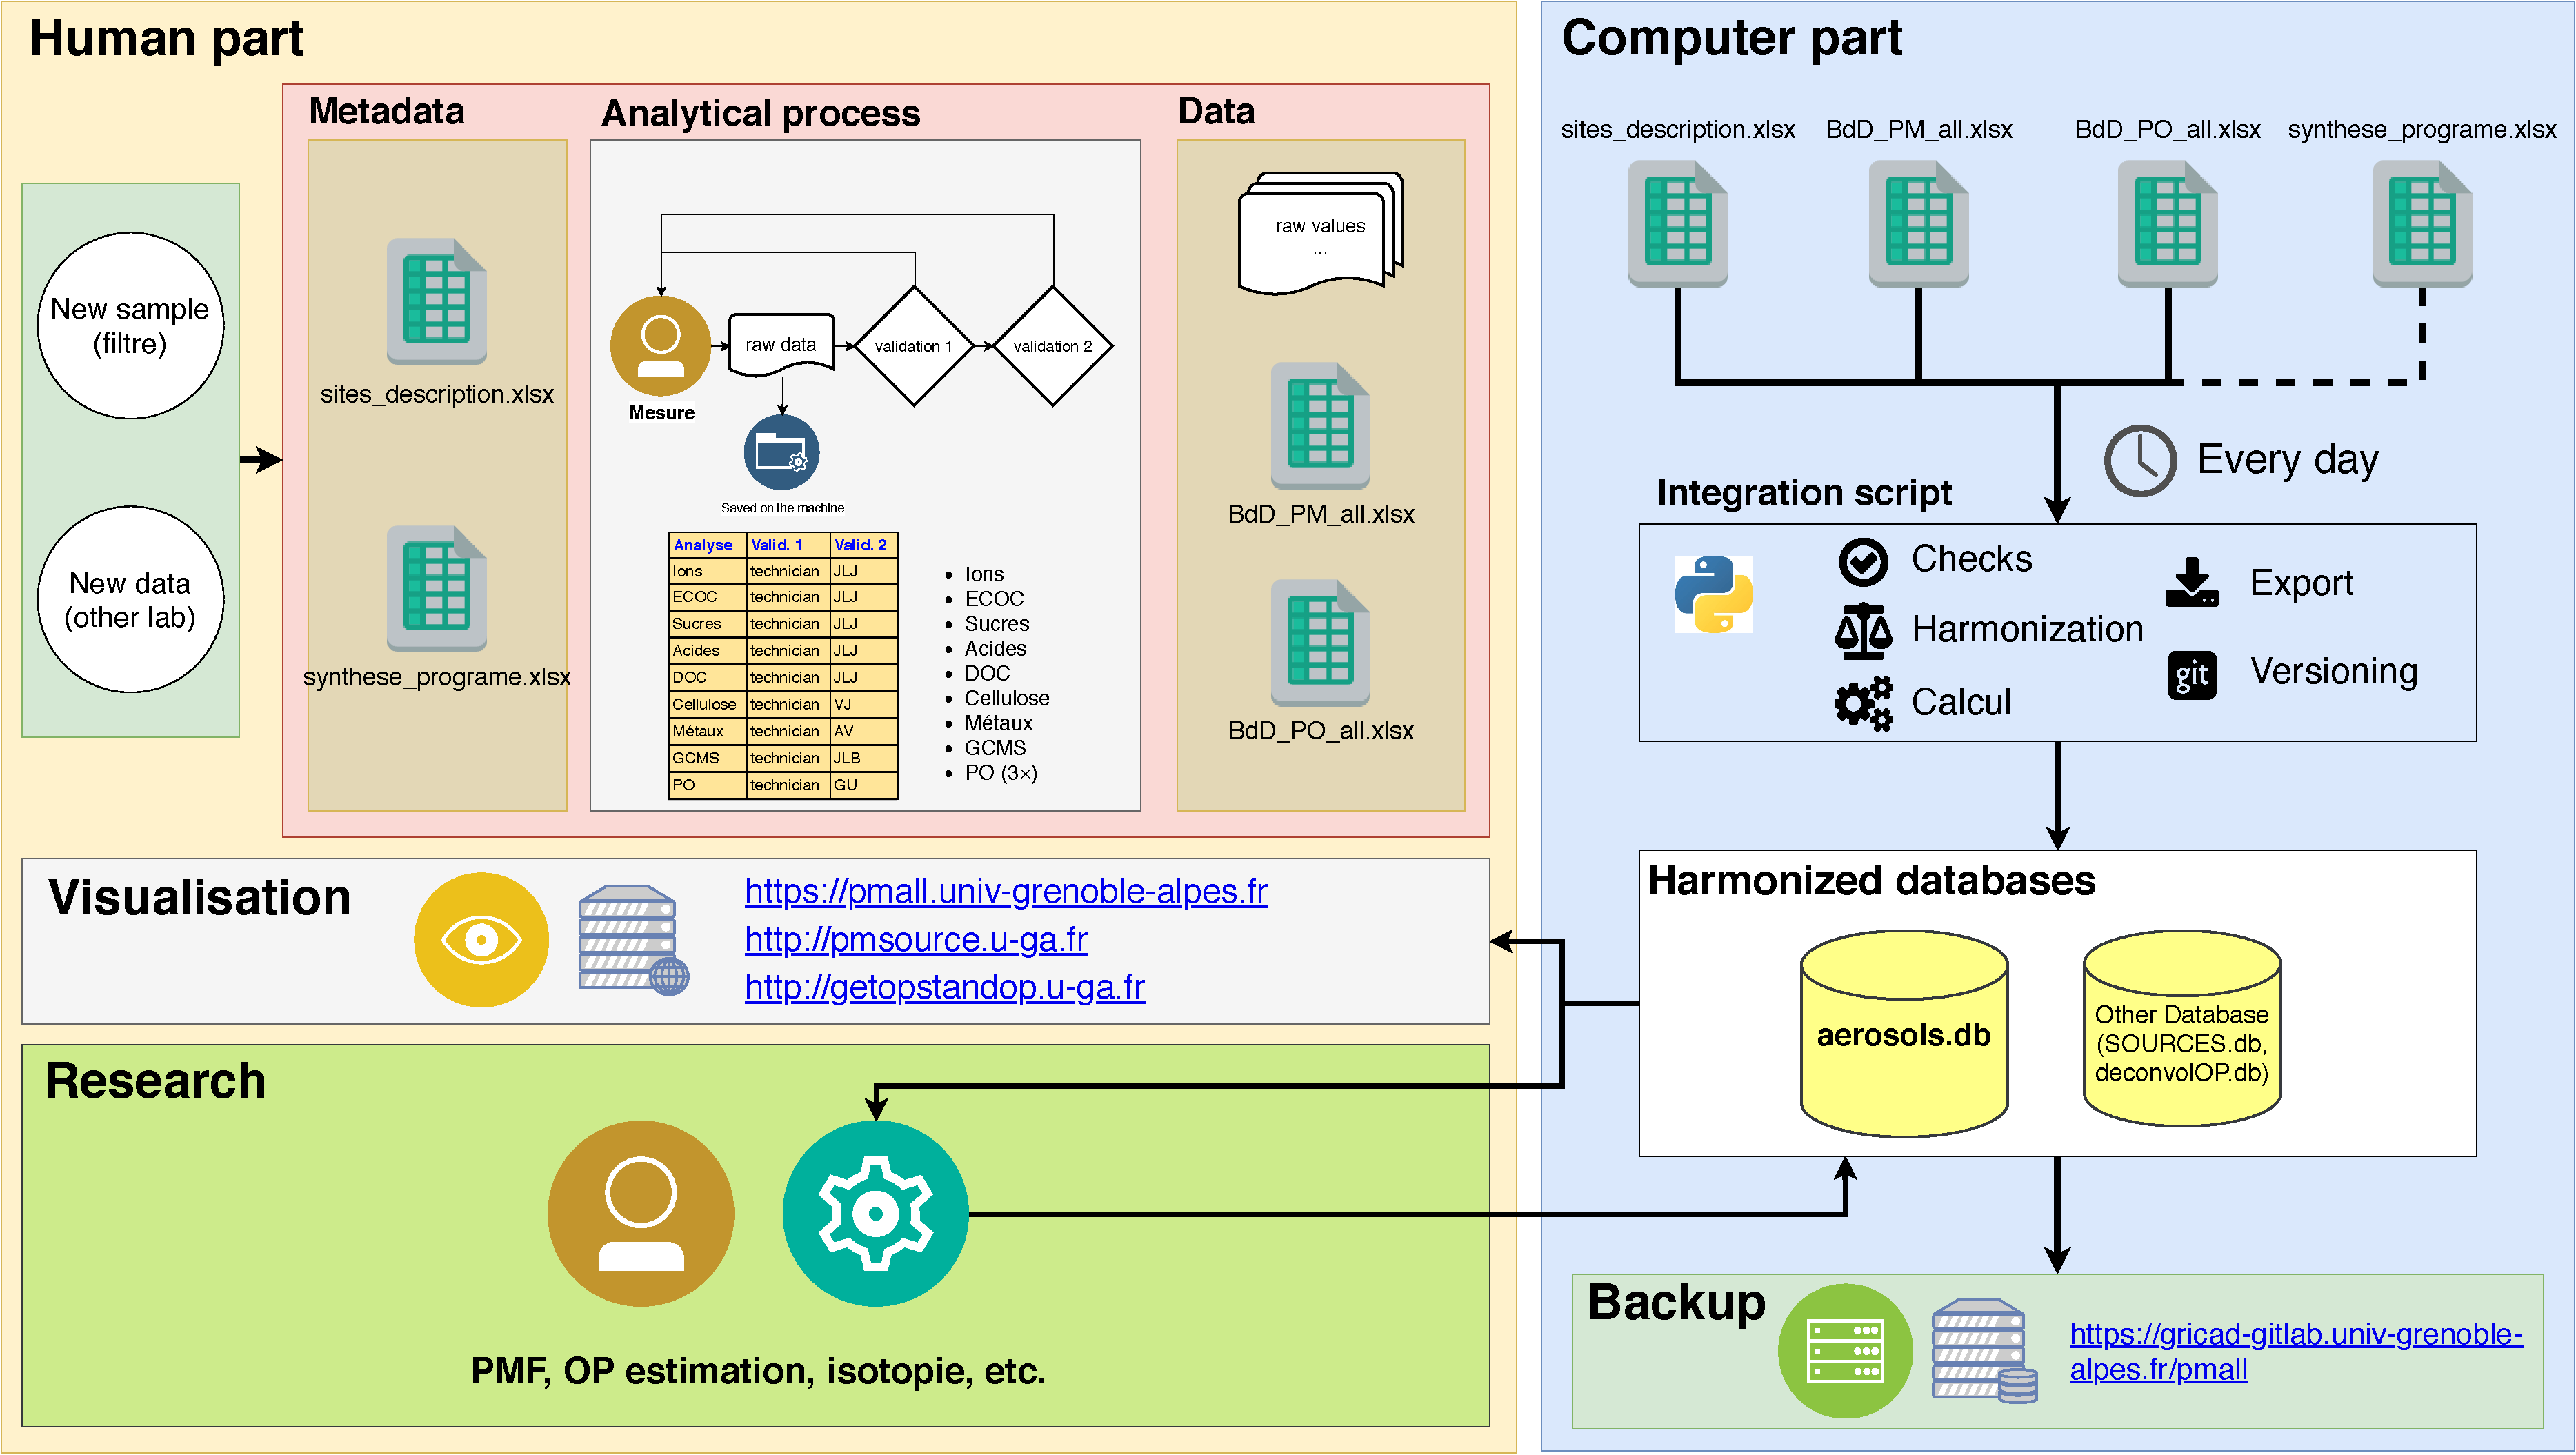
\includegraphics[width=\linewidth]{chapter02/workflow_simple.pdf}
    \caption{Vie d'un échantillon et des données : réception, analyse et enregistrement
        dans la filtrothèque et visualisation, puis utilisation dans les différents
        programmes de recherche.}%
    \label{fig:bdd}
\end{figure}
\end{landscape}

\subsection{Visualisation facilitée}%
\label{sub:visualisation_facilité}

La mise en place d'une interface de visualisation simple et rapide permet une première
exploration facilitée et centralisée en un même lieu
(voir~\ref{fig:figures/chapter02/pmall_example}). Aussi, le croissement de différentes
variables (lieu de prélèvement, espèces chimiques, sources issues des études PMF, mesure
du potentiel oxydant, variables météorologiques, etc.) est grandement simplifié.  De même,
cet outil est évolutif et des fonctionnalités peuvent être très facilement ajoutées. À la
simple évolution temporelle s'est ajoutée la dispersion et moyenne saisonière et mensuelle
ou encore la corrélation entre variable.

Ces différentes étapes de visualisation ne se substitue pas à un travail d'analyses
appronfondi, mais facilite l'analyse exploratoire et la détection d'erreur éventuelle.

\begin{figure}[ht]
    \centering
    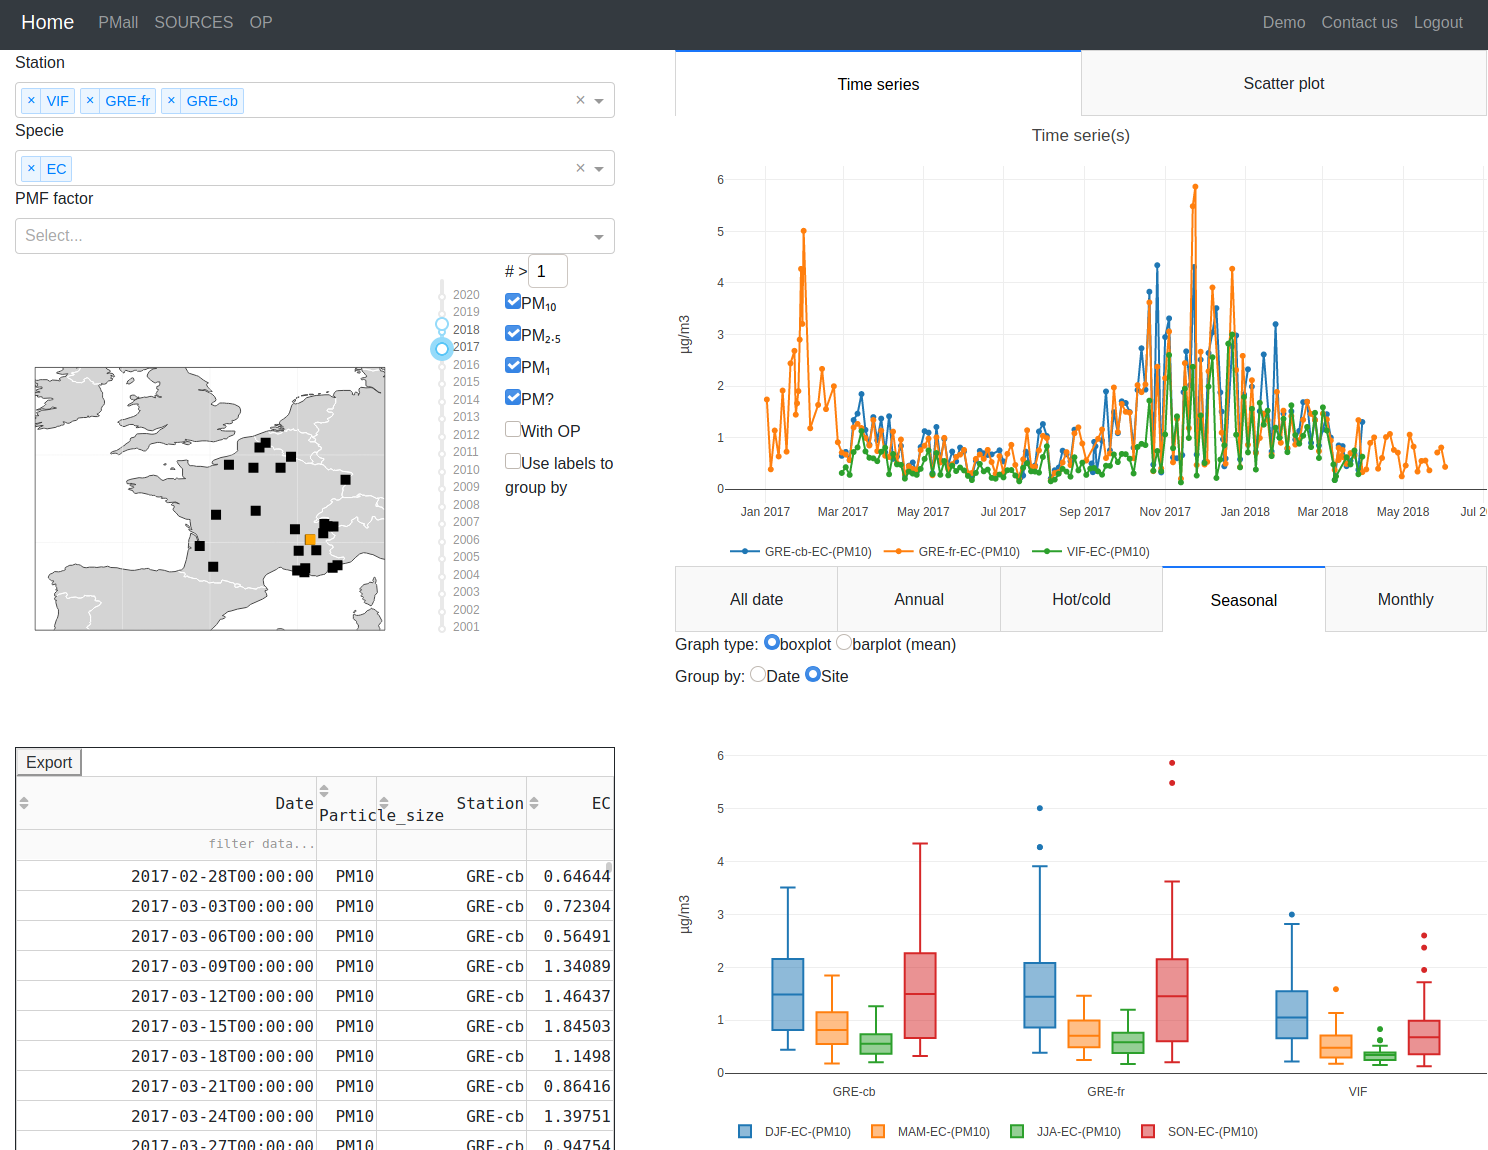
\includegraphics[width=1.0\linewidth]{figures/chapter02/pmall_example.png}
    \caption{Example d'utilisation de l'interface de visualisation de PMall.}%
    \label{fig:figures/chapter02/pmall_example}
\end{figure}


Après avoir présenté dans ce chapitre les différents outils et concepts utilisés ou
développés dans ce travail de thèse, les chapitres suivants vont s'attacher à présenter
les résultats sur les avancées de la déconvolution des sources de PM en ce qui concerne
les contributions massiques
(chapitre~\ref{cha:approfondissement_des_connaissances_des_sources_des_pm}) et les
contributions au potentiel oxydant (chapitre~\ref{cha:estimation_des_sources_de_PO}).





% \clearpage
% \printbibliography[segment=\therefsegment,heading=subbibliography]
%
% \chapter{Approfondissement des connaissances des sources des PM}%
% \label{cha:approfondissement_des_connaissances_des_sources_des_pm}
% \PartialToc
% \clearpage
% 
\section{Introduction}%
\label{sec:introduction}

La PMF étant un modèle d'apprentissage statistique, le regroupement des espèces chimiques
en différent facteurs est sensible à la méthodologie employée et au jeu de variable
utilisé.
Depuis plusieurs années, les travaux du groupes essaient d'évaluer la pertinence de
l'ajout de nouveaux traceurs dans les études PMF, afin de mieux prendre en compte
certaines émissions anthropiques ou biogéniques mais également afin de mieux estimer la
contribution des aérosols secondaires, qu'ils soient organiques ou inorganique.
En plus d'identifier plus précisément ces sources, \cite{emamiEffect2017} ont montré que
l'ajout d'espèce traceuse permet une diminution de l'ambiguité rotationelle pour
l'ensemble des facteurs identifiés. La recherche de nouvelles espèces traceuses est donc
nécessaire pour identifier de nouvelles sources, mais également diminuer l'incertitudes
sur celles déjà bien établies.

À ce titre, le site de Grenoble les Frènes a permis le prélèvement et analyse de composés
organiques (HULIS, hopanes, oxy- et nitro-HAP ainsi que oxy- et nitro-HAPs) permettant de mettre en
évidence la saisonalité de ces composés, tracant différent processus : émissions lié à la
combustion en hiver pour les oxy- et nitro-HAP ainsi que leur transport longue distance
alors que les oxy- et nitro-HAPs semblent quand à eux être d'avantage liés aux processus
d'oxydation secondaires du fait de leur corrélation avec
l'oxalate~\textcite{tomazSources2017a}.
Lors d'études PMF avec ces traceurs \autocite{srivastavaSpeciation2018a}, il ressort bien
qu'une part de ces espèces est associés à la combustion de biomasse mais ont aussi permis
la mise en évidence d'un facteur anthropique secondaire présentant un signal assez
atypique car très ponctuel. Aussi, les processus d'oxydation secondaires de la matière
organique est mieux déterminé et quantifiée, ce qui a permis d'isolé un facteur biogenique
secondaire présentant de forte concentration en été. Quand au trafic routier, la grande
majorité des hopanes se retrouvent dans ce facteurs, alors certains autres composés pour
lesquels des fortes concentrations étaient attendues sont en définitive peu présents dans
ce facteur (notamment pour le 1-nitropyrène \textcite{ringuetDiurnal2012}).

Cependant, certains de ces composés présentent des faibles performances statistiques (i.e.
concentration observées vs reconstruites) et soulèvent différentes intérogations : faut-il
utiliser toutes ces espèces en même temps ? Faut-il aggréger certaines familles de
composés mono-source ? Est-ce que la résolution de 24h est suffisante ?  etc. D'autres
travaux en ce sens ont eu lieu sur le site expérimental de Lens, en sommant par exemple
certaines espèces (hopanes, alcanes, HAP) afin de réduire le nombre d'espèces utilisées
dans la PMF, mais aucun standard n'existe à ce jours et peu d'études rapportent
l'utilisation de ces traceurs dans les PMF.
Aussi, la variabilité spatiale de ces profils semblent être importante. Dans des travaux en
cours de la thèse de Valéria Mardonnez à La Paz, Bolivie, la dynamique de ces composés
dans les PMF permettraient d'identifier jusqu'à 3 facteurs reliés au trafic routier : selon
la source de combustion (diesel ou essence) et émission hors-combustion.

Mais d'autres voies d'ajout de traceurs sont également à l'étude, cherchant à coupler les
mesure sur filtre à d'autres mesures concommitante \parencite{srivastavaSpeciation2019}.
Récemment, la thèse de Florie Chevrier \autocite{chevrierChauffage2016} dans le cadre du
programme DECOMBIO a permis la combinaison de mesure issues de chimie sur filtre,
d'aethalometre (séparant ainsi le BC en combustion de biomasse et combustion fossile) et
mesure de \ce{^{14}C}.

Ainsi, la méthodologie d'utilisation du modèle PMF est encore actuellement en évolution,
et ce chapitre discutera des différentes avancées ou pistes que ma thèse a exploré ces
dernières années.

\section{Validation externe des solutions PMF}%
\label{sec:confrontation_des_solutions_pmf}

Comme discuter précédemment, un modèle doit être évaluer par des mesures externes. Or, il
est compliquer voir impossible de « mesurer » la concentration des sources de PM (c'est
justement le travail demandé à la PMF). On ne peut donc faire que des confrontations
indirectes, à travers d'autres types de mesure ou modèle, chimique ou géophysique, afin
d'estimer la fiabilité d'une solution PMF.

\subsection{Confrontation aux mesures de radiocarbone \ce{^{14}C}}%
\label{sub:14c}

Sur les sites de la vallée de l'Arve dans le cadre du programme DECOMBIO, en plus des mesures
traditionelles sur filtre, \textcite{bonvalotEstimating2016} ont également estimé par
traçage isotopique au radiocarbone \ce{^{14}C} l'origine fossile ou récente du carbone.
Les études PMF sur le site de Passy et Chamonix de \textcite{chevrierChauffage2016},
illustrées figure~\ref{fig:chapter03/radiocarbon_chevrier_winter} ont
montrées une très bonne concordance entre la quantité de carbone provenant de source
fossile estimée par radiocarbone et les facteurs PMF traçant des sources de combustion de
carbone fossil. Réciproquement, le carbone récent est en très bon accord entre les mesures
radiocarbone et PMF.

Cette confrontation à des mesures externes à la PMF conduisant à des résultats concordant
accentue fortement la confiance que l'on peut avoir dans les résultats et la
quantification de la contribution des sources issues de ces analyses.

\begin{figure}[ht]
    \centering
    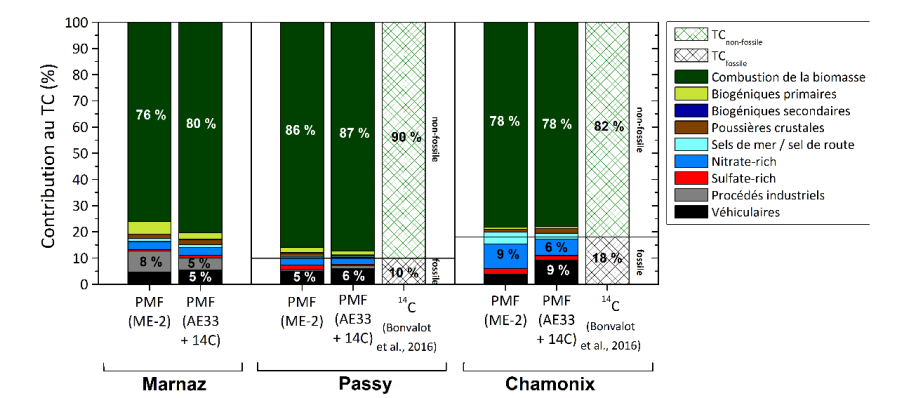
\includegraphics[width=1.0\linewidth]{chapter03/radiocarbon_chevrier_winter.png}
    \caption{Contributions relatives au carbone total en moyennes hivernales des sources
        de \PMdix identifiées lors de la thèse de \textcite{chevrierChauffage2016} par les
        différentes approches PMF et contributions des parts fossile et non-fossile
        obtenues par l’analyse du radiocarbone de \textcite{bonvalotEstimating2016}.
    Source: \textcite[figure 75]{chevrierChauffage2016}}%
    \label{fig:chapter03/radiocarbon_chevrier_winter}
\end{figure}

\subsection{Confrontation mesure sur site récepteur et origine géographique}%
\label{sub:confrontation_mesure_sur_site_recepteur_et_origine_geographique}

Les facteurs PMF étant déterminer au niveau du site recepteur mais n'étant pas
nécessairement émis à cet endroit spécifique, il est également possible d'estimer leur
provenance géographique et leur vraisemblance. Nous verrons d'abord le cas simple de la
rose des polluants, avant d'expliciter plus en avant la méthode PSCF.


\subsubsection{Cas simple : la rose des polluants}%
\label{ssub:cas_simple_la_rose_des_polluants}

L'un des moyens les plus simples pour cela est de coupler des mesures de direction et
vitesse de vent et d'établir une rose des polluants. J'ai pu utiliser ce procédé à des
fins exploratoires lors de ma thèse, ce qui m'a conduit à contribuer au développement de
\href{https://github.com/python-windrose/windrose/}{windrose}~\autocite{scls19frPythonwindrose2019}.
Cependant, cette méthode n'est utile que pour la détermination de source proche du site
récepteur car dès lors que l'on s'en éloigne, l'orientation et vitesse des vents varient
et l'hypothèse de déplacement uniforme de la masse d'air est invalidée.  Or, il est
courant que les aérosols proviennent de sources non locales, limitant l'utilisabilité de
cette méthode.


\subsubsection{Prendre en compte l'histoire de la masse d'air : PSCF}%
\label{sub:prendre_en_compte_l_histoire_de_la_masse_d_air_PSCF}

Pour s'affranchir de la limitation des rose des vents, il est possible d'utiliser les
rétrotrajectoires complètes des masses d'air pour remonter aux sources géographiques
potentielles, mais également de coupler ces trajectoires à des informations
physico-chimiques comme la concentration en polluants observés sur le site récepteur, la
présence de pluie sédimentant les aérosols par dépôt humide ou encore la hauteur de la
masse d'air.

L'une des méthodes les plus largement utilisée dans la littérature est la \textit{Potential
source contribution function} (PSCF), permettant de combiner des ensembles de trajectoires à
des modèles récepteurs. Le principe consiste à calculer les rétrotrajectoires d'un site
récepteur donné et d'associer à chacune d'elle la concentration du polluant ou de la
source considéré le jour de son passage au niveau du site récepteur. En discrétisant les
trajectoires en 1 point toutes les X minutes ou heures et en appliquant une grille
régionale, il est alors possible de dénombrer combien de rétrotrajectoires sont passés par
chacune des grilles.  Le ratio du nombre de trajectoire associée à une forte concentration
aux coordonnées $i$, $j$, noté $m_{ij}$, par le nombre total de trajectoire étant passé
par ces coordonnés notées $n_{ij}$, nous donne une probabilité de provenance géographique
de ce composé ou source pour les coordonnées $i$, $j$, noté $PSCF_{ij}$ :
\begin{align}
    \label{eq:PSCF}
    PSCF_{ij} &= \frac{m_{ij}}{n_{ij}}.
\end{align}

Des améliorations ont été apportées à cette méthode afin de prendre en compte les cellules
ayant un faible pourcentage de passage de rétrotrajectoires, augmentant artificiellement
le ratio $\frac{M}{N}$. Une manière de contrebalancer ce biais et d'ajouter une fonction
poids, dépendant de la fréquence de passage des rétrotrajectoires sur chacune des
cellules. Dans la figure~\ref{fig:chapter02/PSCF_method}, illustrant la PSCF, on voit que
la cellule où 2 rétrotrajectoires sont passés se voit attribuer la même probabilité que
celles avoisinantes, où seule une rétrotrajectoire a résidé. Or, il serait plus pertinent
d'avoir une probabilité plus forte pour cette cellule, indiquant que chaque
rétrotrajectoire ayant résidé à ces coordonnées est riche du composé suivit.  Différentes
fonctions poids existent, le plus souvent présentant différents seuils en fonction du
nombre de rétrotrajectoires par cellule~\autocite{bressiSources2014,petitSources2019}.

Aussi, pour avoir une représentativité statistique suffisante des sources potentielles, il
est nécessaire de calculer un grand nombre de rétrotajectoire, correspondant à chacun des
jours de prélèvement sur le site récepteur.


\begin{figure}[ht]
    \centering
    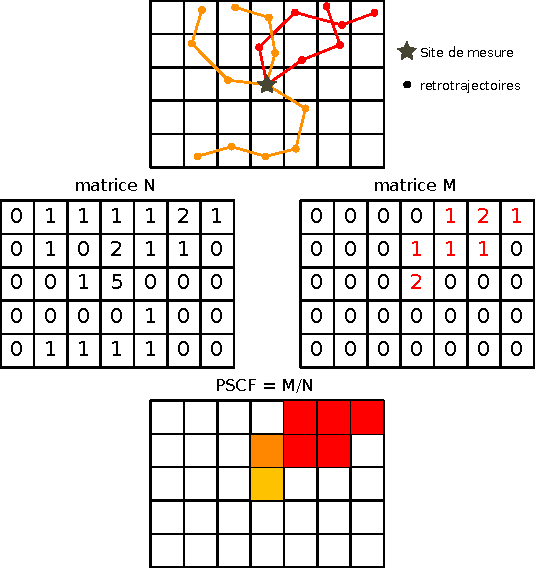
\includegraphics[width=0.9\linewidth]{chapter03/PSCF_method.pdf}
    \caption{Illustration de la méthode PSCF : les rétrotrajectoires depuis le site de
        mesure sont calculées, celles associées à une concentration seuil sont
        représentées en rouge, les autres en orange. Les matrices N et M s'obtiennent par
        simple décompte du nombre de rétrotrajectoires passés dans chaque cellule de
        taille prédéfinies, puis le ratio nous donne une estimation de l'origine
    géographique, représentée ici terme d'intensité de rouge.}%
    \label{fig:chapter02/PSCF_method}
\end{figure}

\subsubsection{Automatisation et simplification : pyPSCF}%
\label{ssub:automatisation_et_simplification_pypscf}

Ces étapes fastidieuses de calcul des rétrotrajectoires et de PSCF ont été automatisés
dans un paquet python, pyPSCF\footnote{Dépot git pyPSCF:
\url{https://gricad-gitlab.univ-grenoble-alpes.fr/webersa/pyPSCF}}, permettant le
traitement d'un grand nombre de rétrotrajectoire en utilisant le modèle lagrangian
HYSPLIT et calculant de manière facilité une PSCF en un site donné, en variant notamment
les différents paramètres succeptibles d'influencer le modèle.

Également, et de manière similaire à ZeFir de \textcite{petitUserfriendly2017}, pyPSCF
propose une interface utilisateur permettant une interaction facilité.

\subsubsection{Application de la PSCF}%
\label{ssub:application_de_la_pscf}

\paragraph{Importance et origine géographique du MSA ? (Golly et al. 2019)}%
\label{par:origine_terrestre_ou_marine_du_msa_}

Comme expliqué précemment, une part importante des aérosols provient de sources
secondaires, c'est-à-dire du vieillissement et des réactions dans l'atmosphère. Une part
importante de ces aérosols secondaires sont d'origines organiques. Les travaux
de~\textcite{gollyOrganic2019}, auxquels j'ai pris part, s'attachent notamment à la
quantification de cette matière organique secondaire sur 5 sites ruraux en France
pendant l'année 2013, par la mesure de deux espèces issues de processus secondaires : le
MSA et l'oxalate.  Nous avons pu montrer que le MSA, considéré comme provenant de
l'oxydation du DMS, peut contribuer jusqu'à 10 à 20\% de l'OC en période chaude,
indiquant une forte proportion d'aérosols organiques secondaires durant l'été. Mais
surtout, le MSA est considéré comme provenant des émissions de DMS du phytoplanction
marin, au point qu'il est proposé comme méthode de séparation entre le sulfate d'origine
marine et ses autres provenances.

En conduisant une analyses PSCF sur les 25\% des jours les plus fortement chargés en MSA,
nous avons pu confirmer l'importance marine de ce composé, mais également montrer qu'une
part non négligeable semble provenir d'environnement terrigène (voir
figure~\ref{fig:chapter03/golly_PSCF_MSA}), confortant les études suggérants des
processus d'émissions du MSA par des sources biologiques
terrestres~\autocite{bozzettiArgon2017}, pouvant provenir des forêts ou des
sols~\autocite{jardineDimethyl2015,miyazakiSeasonal2012}.

L'une des implications directes de ces travaux résulte en l'ajout systématique du MSA
comme variable d'entrée des études PMF, quelque soit leur localisation. En effet, le
signal du MSA est clairement distinct des autres espèces chimiques mesurées et représente
également une part important de la matière organique. Cette espèce est donc a minima
traceuse de processus secondaires présents sur l'ensemble de l'europe occidentale.

\begin{figure}[ht!]
    \centering
    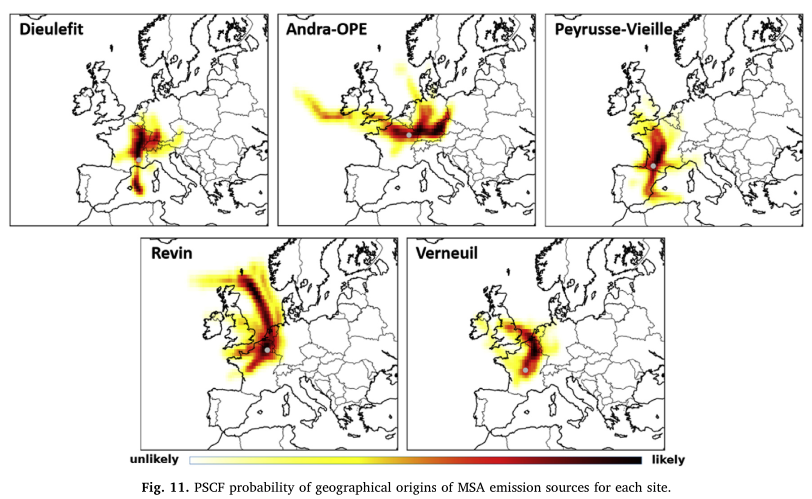
\includegraphics[width=0.9\linewidth]{chapter03/golly_PSCF_MSA.png}
    \caption{Probabilité de l'origine géographique du MSA, issue de l'article
        de~\textcite{gollyOrganic2019}. Bien que l'on retrouve l'origine marine du MSA,
        les sites de Dieulefit, OPE ou Peyrusse-Vieille indiquent également une forte
        probabilité d'origine terrestre de ce composé.}%
    \label{fig:chapter03/golly_PSCF_MSA}
\end{figure}

\paragraph{Confrontation PSCF -- PMF}%
\label{par:confrontation_pscf_pmf}

Une autre utilisation de la PSCF consiste à croiser les informations issues de la PSCF et
des PMF.
En effet, il n'existe pas de moyen simple de valider le sens géochimique d'une solution
PMF autrement que l'expertise et les connaissances de l'utilisateur.

Pour estimer la fiabilité de la solution obtenue, il est possible de conduire une
étude PSCF sur les différents facteurs identifiés. On s'attend à ce que le
facteur \textit{sel de mer} provienne géographiquement d'un océan ou d'une mer par
exemple.

Un exemple d'utilisation de ce procédé est expliqué et illustré dans la section dédié aux
PMF et isotopie, section~\ref{sub:isotopie}.



\section{Incertitudes associées aux PMF}%
\label{sub:incertitudes_associées}

Le modèle PMF est maintenant relativement courrament utilisés dans le domaine de la
qualité de l'air. Seulement, peu d'étude rapportent en même temps que leur solution
finale, les incertitudes associées. Or, le solveur ME-2 permet l'estimation de ces
incertitudes à travers les méthodes de bootstrap et de displacment (voir
section~\ref{par:incertitudes}).

Seulement, ces incertitudes ne sont rapportées par l'EPAPMF5.0 que pour les concentrations
des espèces chimiques des différents facteurs et non pour leurs contributions temporelles.
Notamment, leur de l'estimation de la variabilité via bootstrap, les différents facteurs
sont attribués aux facteurs de références d'après leur corrélation temporelle (par défaut
$r > 0.6$), mais seul les profils chimiques sont rendu à l'utilisateur par la suite.
Une solution serait de manuellement explorer 100 solutions PMF, avec ou sans tirage
aléatoire des échantillons, pour estimer respectivement la variabilité provennant du modèle
statistique ou de la représentativité du jeu de donnée. Malheureusement, cette
répétabilité est beaucoup trop fastidieuse à faire à la main et ne peut pas s'automatiser à
partir de l'EPAPMF5.0. Or, il s'agit de l'implémentation du ME-2 le plus largement
utilisée. C'est pourtant une besoin important lors de la transférabilité de nos recherches
vers l'opérationnel, avec des questions très pratique cherchant l'incertitude
sur la contribution de telle source pour tel jours de pic de pollution en particulier.

Une ``astuce'' consiste alors a réestimer la variabilité des contributions temporelles
$X_{err}$ à partir de la variabilité de la composition chimique des profiles, i.e. en gardant
$G$ fixe (celle de référence, $G_{ref}$) mais en utilisant les profiles $F_{err}$ issue
des bootstraps et ambiguité rotationelle :
\begin{align}
    \label{eq:hack_unc}
    X_{err} &= G_{ref} \times F_{err}.
\end{align}

Même si en théorie pour la méthode du bootstrap à la fois $G$ et $F$ doivent
évoluer en même temps, cela donne une première estimation de la gamme d'incertitude pour
chaque espèce et chaques jours d'observation.

Cette visualisation, présentée à titre d'exemple pour la PMF de Vif
figure~\ref{fig:chapter03/vif_nitraterich_all} permet de rapidement se rendre compte du
type d'incertitude prépondérant pour chacune des espèces (représentativité de
l'échantillonage et ambiguité rotationelle) mais également de la gamme de valeur possible
pour chaque jours étant donnée les incertitudes estimées.

\begin{figure}[ht]
    \centering
    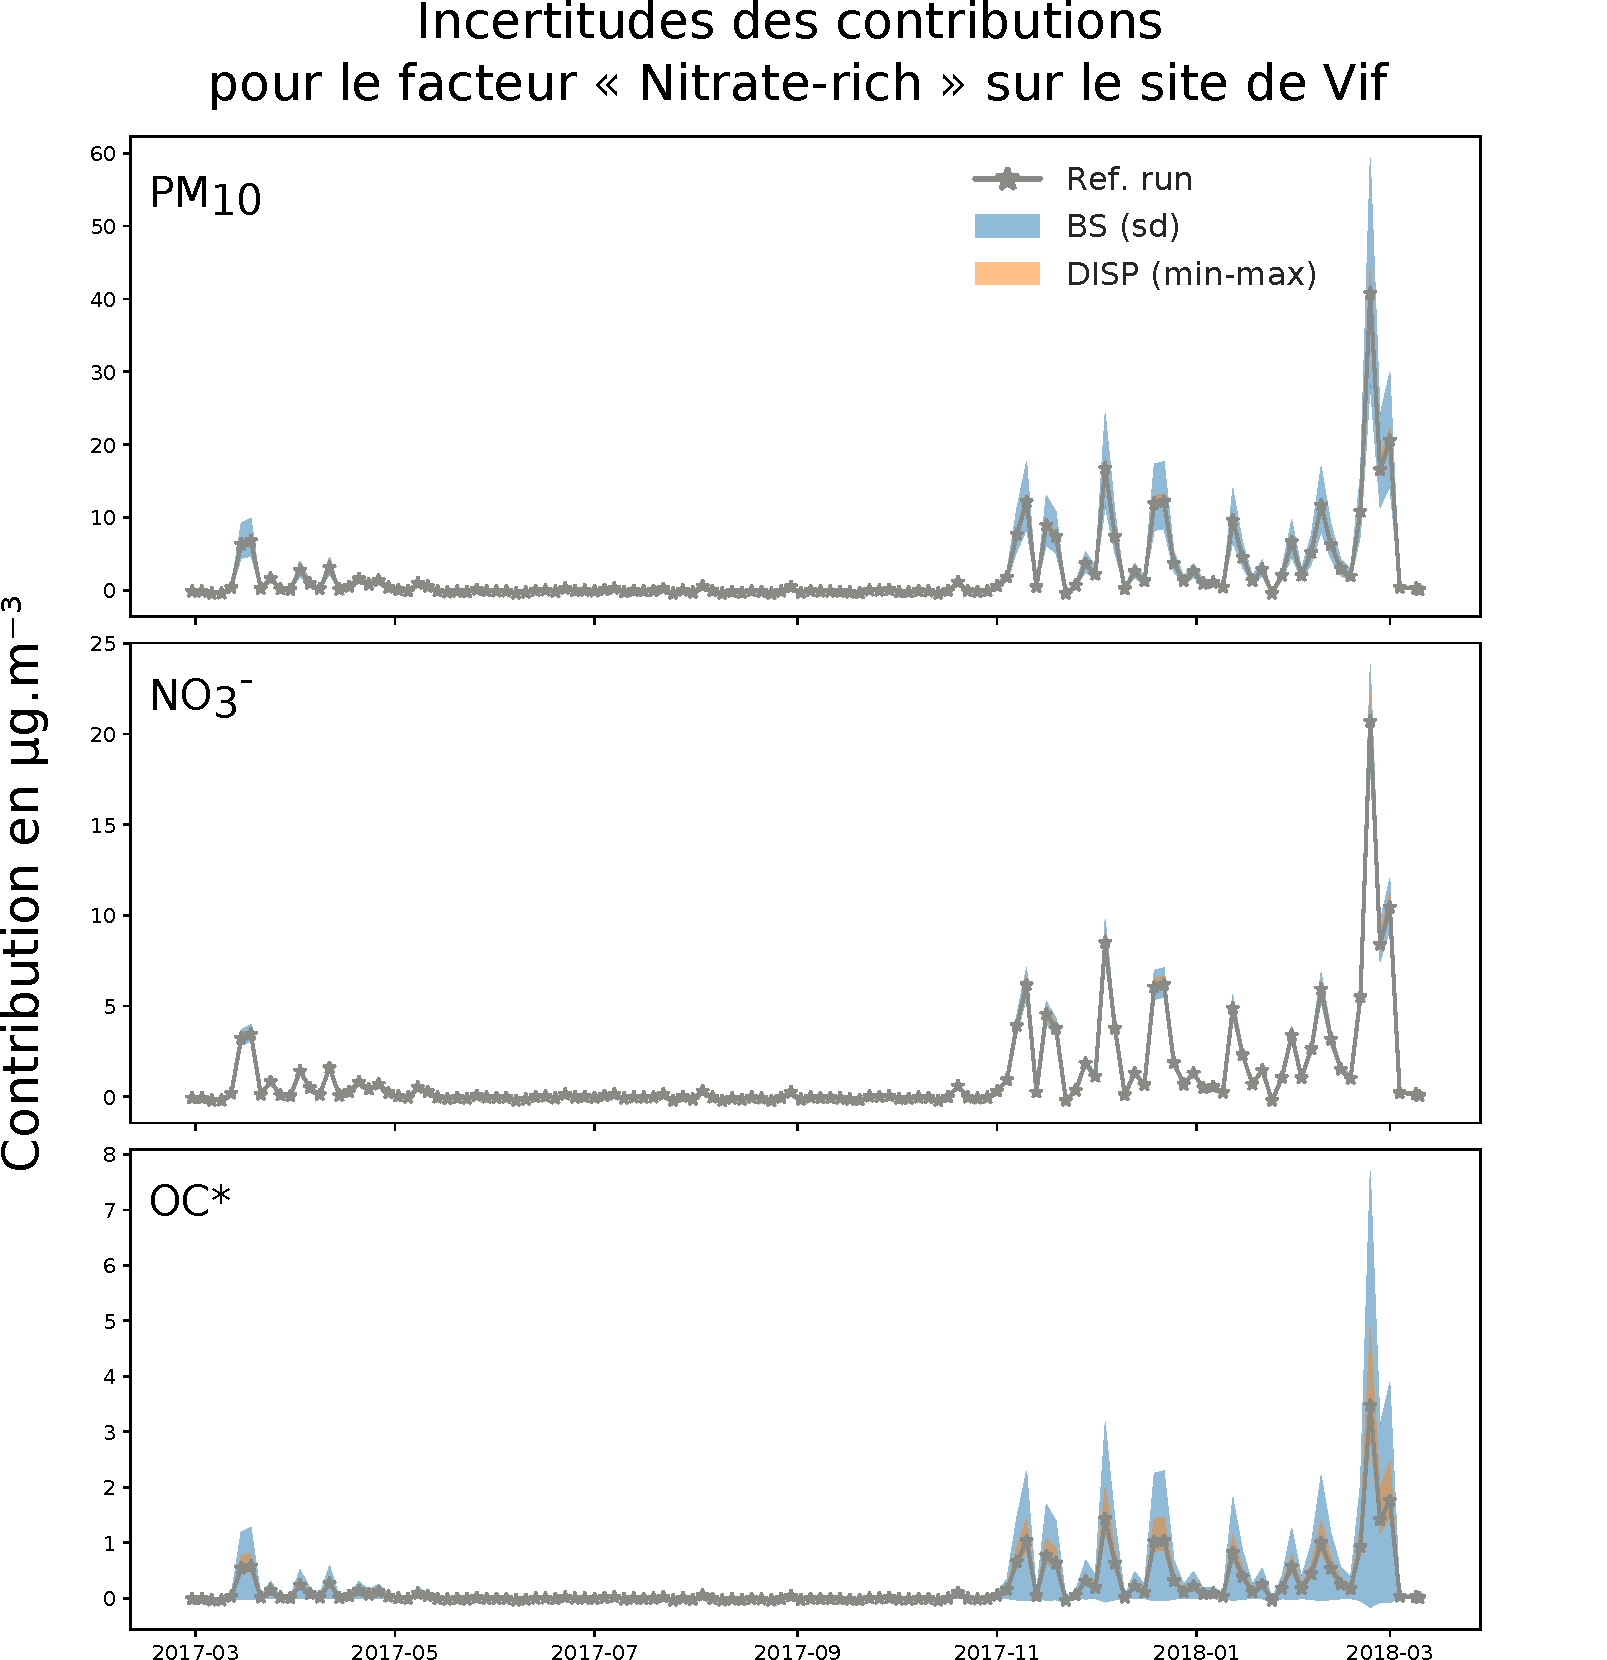
\includegraphics[width=0.8\linewidth]{chapter03/vif_nitraterich_all.pdf}
    \caption{Incertitudes temporelles des concentrations de \PMdix, \NOt et OC* dans le
    facteur Nitrate-rich de Vif estimée par boostrap (écart type de 100 bootstrap en bleu)
et displacment (min et max en orange). La solution de référence est représenté par les
trais et étoiles grisent.}%
    \label{fig:chapter03/vif_nitraterich_all}
\end{figure}


\section{Comparabilité des solutions}%
\label{sub:comparabilité_des_solutions}

Une problématique récurrente lors de l'utilisation des PMF est de se demander si les
profils que l'on obtient seraient nommés de la même façons par d'autres utilisateurs, et
si oui, comment peut-on évaluer la proximité géochimique de facteurs identiquement nommés
en différents endroits (spatiallement ou temporellement).

Les travaux de \cite{belisNew2015a} suggèrent l'utilisation conjointe de 2
métriques permettant d'estimer la distance géochimique entre 2 profiles de facteurs.

\subsection{Méthodologie}%
\label{sub:méthodologie}

\paragraph{Distance de Pearson}%
\label{par:distance_de_pearson}

La distance de Pearson (\textit{Pearson distance} PD) estime la proximité entre 2 série de
donnée en utilisant leur corrélation de Pearson, soit :
\begin{align}
    \label{eq:PD}
    PD &= 1 - r^2
\end{align}
avec $r$ la correlation entre les 2 séries de données. Pour les profiles chimiqes des
facteurs, il s'agit de la concentration relative des espèces chimiques les constituants
(i.e. pourcentage massique de chacune des espèces).

Seulement, cette distance est très sensible aux extrêmes du fait de sa dépendance au
coefficient de correlation. Ainsi, si seul l'OC est similaire pour les 2 profiles mais la
totalité des métaux présentent des concentrations très différentes, alors le PD pourra
être acceptable car l'OC présente des concentrations relative bien supérieure à celles
des métaux (voir figure~\ref{fig:chapter03/PD_belis2015a}).
De plus, la distance de Pearson ne teste que l'hypothèse de relation linéaire entre les
deux profiles, et non leur égalité stricte.

\begin{figure}[ht]
    \centering
    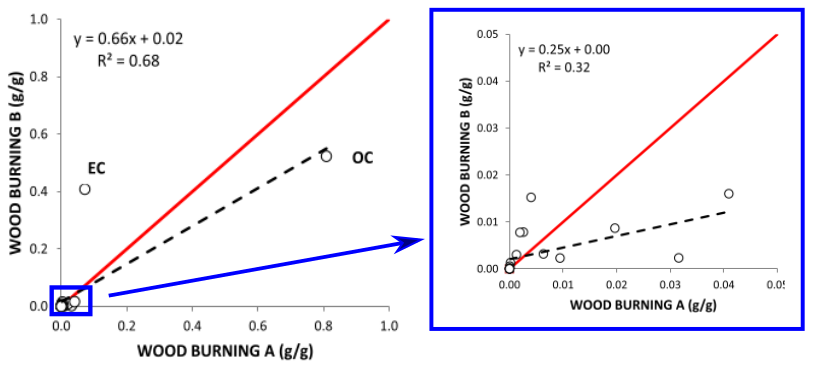
\includegraphics[width=1.0\linewidth]{chapter03/PD_belis2015a.png}
    \caption{Mesure de la distance de pearson de 2 sources \textit{wood burning}. L'image
        de droite montre l'influence des espèces dominant la masse pour le calcul du PD, alors
        qu'en leur absence, le PD change drastiquement (image de droite). Source: adapté de
        \cite[figure 3]{belisNew2015}.
}%
    \label{fig:chapter03/PD_belis2015a}
\end{figure}


\paragraph{Distance identitaire standardisée}%
\label{par:distance_identitaire_standardisée}

Pour répondre aux problèmes soulevés par la distance de Pearson, \textcite{belisNew2015}
propose l'utilisation de la distance identitaire standardisée (\textit{Standardized
Identity Distance} SID). Sa formulation a légèrement évoluée entre son expression
initiale par \textcite{belisNew2015} et celle actuellement utilisée par SPECIEUROPE
\autocite{pernigottiSPECIEUROPE2016,pernigottiDeltaSA2018}.

L'idée principale consiste à exprimer la distance entre chaque pair d'espèce $i$ pour les 2
profiles considérés $x$ et $y$ et la droite unitée, noté $ID_i$ pour \textit{identity
distance}, telle que:
\begin{align}
    \label{eq:IDi}
    ID_i &= \frac{1}{\sqrt{2}}|x_i - y_j|.
\end{align}
Aussi, afin de prendre en compte de manière homogène toutes les espèces et s'extraire du
biais sur-considérant les espèces prépondérantes à la masse, l'ID est normalisée par une
valeure proportionnelle à la moyenne de la masse de l'espèce $i$ dans le facteur $x$ et
$y$, appelée \textit{maximum acceptable distance} MAD, telle que:
\begin{align}
    \label{eq:MAD}
    MAD_i &= k \frac{1}{2}(x_i + y_i).
\end{align}
Ce procédé est illustré figure~\ref{fig:chapter03/SID_belis2015a}.

La SID est la moyenne de la somme des ratio entre l'ID et le MAD, telle que:
\begin{align}
    \label{eq:SIDi}
    SID &= \frac{1}{m}\sum_i^m\frac{ID_j}{MAD_j},
\end{align}
soit :
\begin{align}
    \label{eq:SID}
    SID &= \frac{\sqrt{2}}{km} \sum_i^m \frac{|x_i - y_i|}{x_i + y_i}.
\end{align}

\begin{figure}[ht]
    \centering
    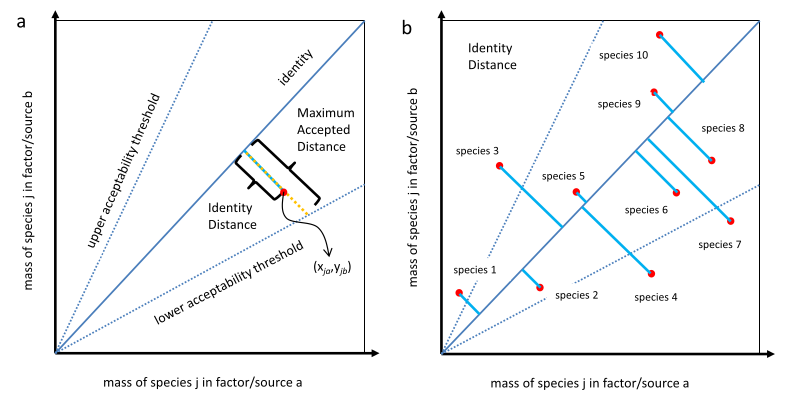
\includegraphics[width=0.9\linewidth]{chapter03/SID_belis2015a.png}
    \caption{Illustration schématique de la distance SID. Légende originelle:
        Geometric representation of the identity distance (ID) as an indicator of
        similarity between two factor/source profiles. Left pane: $ID_{j,ab}$ between
        factor/sources $a$ and $b$ for species $j$ with acceptability thresholds (dotted lines);
        the dot represents point ($x_{ja}$, $y_{jb}$ ). Right pane: comparison of two
        hypothetical factor/sources with 10 common species.
        Source: \cite[figure 2]{belisNew2015}
}%
    \label{fig:chapter03/SID_belis2015a}
\end{figure}

\subsection{Implémentation et utilisation}%
\label{sub:implémentation_et_utilisation}

Ces 2 métriques de distances entre profiles sont utiles pour l'aide à l'identification
d'un nouveau profiles, notamment via SPECIEUROPE. Cependant, toutes les espèces chimiques
que nous utilisons ``en routine'' ne sont pas nécessairement présente dans les profiles de
SPECIEUROPE. Aussi, SPECIEUROPE nous permet de comparer aux profiles déjà existant, et non
par exemple des PMF sur 2 sites non encore dans la base de donnée SPECIEUROPE.

Ainsi, pour comparer les profiles chimiques issues d'une même méthodologie PMF (même
variables d'entrée, même contraintes, etc) à différents lieux, j'ai réimplenté une version
de deltaTool en python\footnote{Disponible dans le paquet
    \href{https://pypi.org/project/py4pm/}{py4pm}, dépot git:
\url{https://gricad-gitlab.univ-grenoble-alpes.fr/webersa/py4pm}
} permettant une
utilisation plus flexible et une comparabilité des PMF conduitent pendant ma thèse.

Le choix de $k$ de l'Eq.~\ref{eq:SID} pour le MAD a été porté à 1, similairement à
\cite{pernigottiDeltaSA2018}, en absence d'information a priori sur la variabilité de ces
profiles.

La question de la comparabilité des profiles s'est posé majoritairement à 3 moments de ma
thèses :
\begin{enumerate}
    \item Comparer 15 PMF utilisant une méthodologie harmonisée en France (project
        SOURCES);
    \item Étudier la variabilité fine échelle (i.e. à l'échelle d'une métropole) à travers
        3 sites de prélèvement dans un rayon de \SI{15}{\kilo\m} autour de Grenoble, France
        (projet Mobil'Air);
    \item Évaluer l'impact de l'ajout de traceurs organiques (acide pinic, phtalic,
        3-MBTCA et cellulose) par rapport à une PMF ``standard'' sur les 3 sites
        Grenoblois (projet Mobil'Air).
\end{enumerate}

Le premier item sera abondamment traité dans la section~\ref{sec:sources} et
\textcite{weberComparison2019}, tandis que les 2 autres font l'object d'un article en
cours de soumission par \textcite{borlazaFinescaleinprep.} et sont détaillés succintement
dans la section~\ref{sub:processus_secondaires}.

\section{Amélioration des solutions PMF par ajout de traceurs spécifiques}%
\label{sec:amélioration_des_solutions_pmf}

\subsection{Apport de l'isotopie de l’azote sur la caractérisation des sources de pollution émettrices d’ammonium}%
\label{sub:isotopie}
\todo{contextualiser ces recherches}

\subsubsection{Problématique}%
\label{ssub:problématique}

Dans de nombreuses PMF, il est rapporté un facteur secondaire inorganique contennant une
grande part du sulfate, du nitrate et de l'ammonium, indiquant la présence de sulfate
d'ammonium \ce{SO4(NH4)2} et nitrate d'ammonium \ce{NO3NH4}. Ces deux facteurs sont
également souvent distinct, formant un facteur ``sulfate rich'', présentant le sulfate
d'ammonium mais sans nitrate, et ``nitrate rich'' présentant du nitrate d'ammonium mais
sans sulfate.

Le facteur nitrate rich présente des émissions très saisonnière, responsable des grands
événements de dépassement des seuils d'alerte printanier. Seulement, s'agissant d'un
facteur secondaire issu de condensation des NOx et de l'ammoniac \ce{NH3}, sa provenance
n'est pas clairement établit, même sur les NOx sont supposés venir du traffic routier et
l'ammoniac de l'agriculture.

\subsubsection{Objectifs et méthods}%
\label{ssub:objectif}

Dans ce cadre, le programme INACS de l'ADEME a permis les mesures de
l'isotopie de l'azote du nitrate et de l'ammonium sur des cylces annuel complet à X sites.
Parallèlement, les mesures de la signature isotopique à l'émission de différentes sources
ont été faite à l'IGE, notamment en tunnel et à l'émission de cheminée (combustion de
biomasse domestique). Différentes prélèvement issus de sources agricoles (fumier, fertilizant
de synthèse, etc) ont également été analysés.

L'isotopie est une technique connue permettant l'estimation des sources d'émission,
seulement, il n'est pas possible de l'utiliser tel quel dans une analyse PMF et donc
d'avoir cette information pour identifier plus précisement la source nitrate rich.
En effet, la PMF résout une équation d'équilibre des masses et est donc purrement
additive. Or, l'isotopie se traduit par une équation de mélange, résultant en une moyenne
pondérée de la signature isotopique des sources par leur contribution.

\subsubsection{Principaux résultats}%
\label{ssub:principaux_résultats}


\subsection{Émission biogénique primaire}%
\label{sub:émission_biogénique_primaire}

\subsection{Processus secondaires}%
\label{sub:processus_secondaires}

\section{SOURCES}%
\label{sec:sources}

\subsection{Introduction}

\subsection{Comparison of PM\textsubscript{10} sources profiles at 15 french sites using a harmonized constrained positive matrix factorization approach}%
\label{sub:article}

\subsection{Conclusion}%
\label{sub:conclusion}



% \includepdf[pages=-,scale=0.9,pagecommand={\pagestyle{fancy}}]{chapters/sources.pdf}

% \subsection{Supporting Information}%
% \label{sub:supporting_information}
%
% 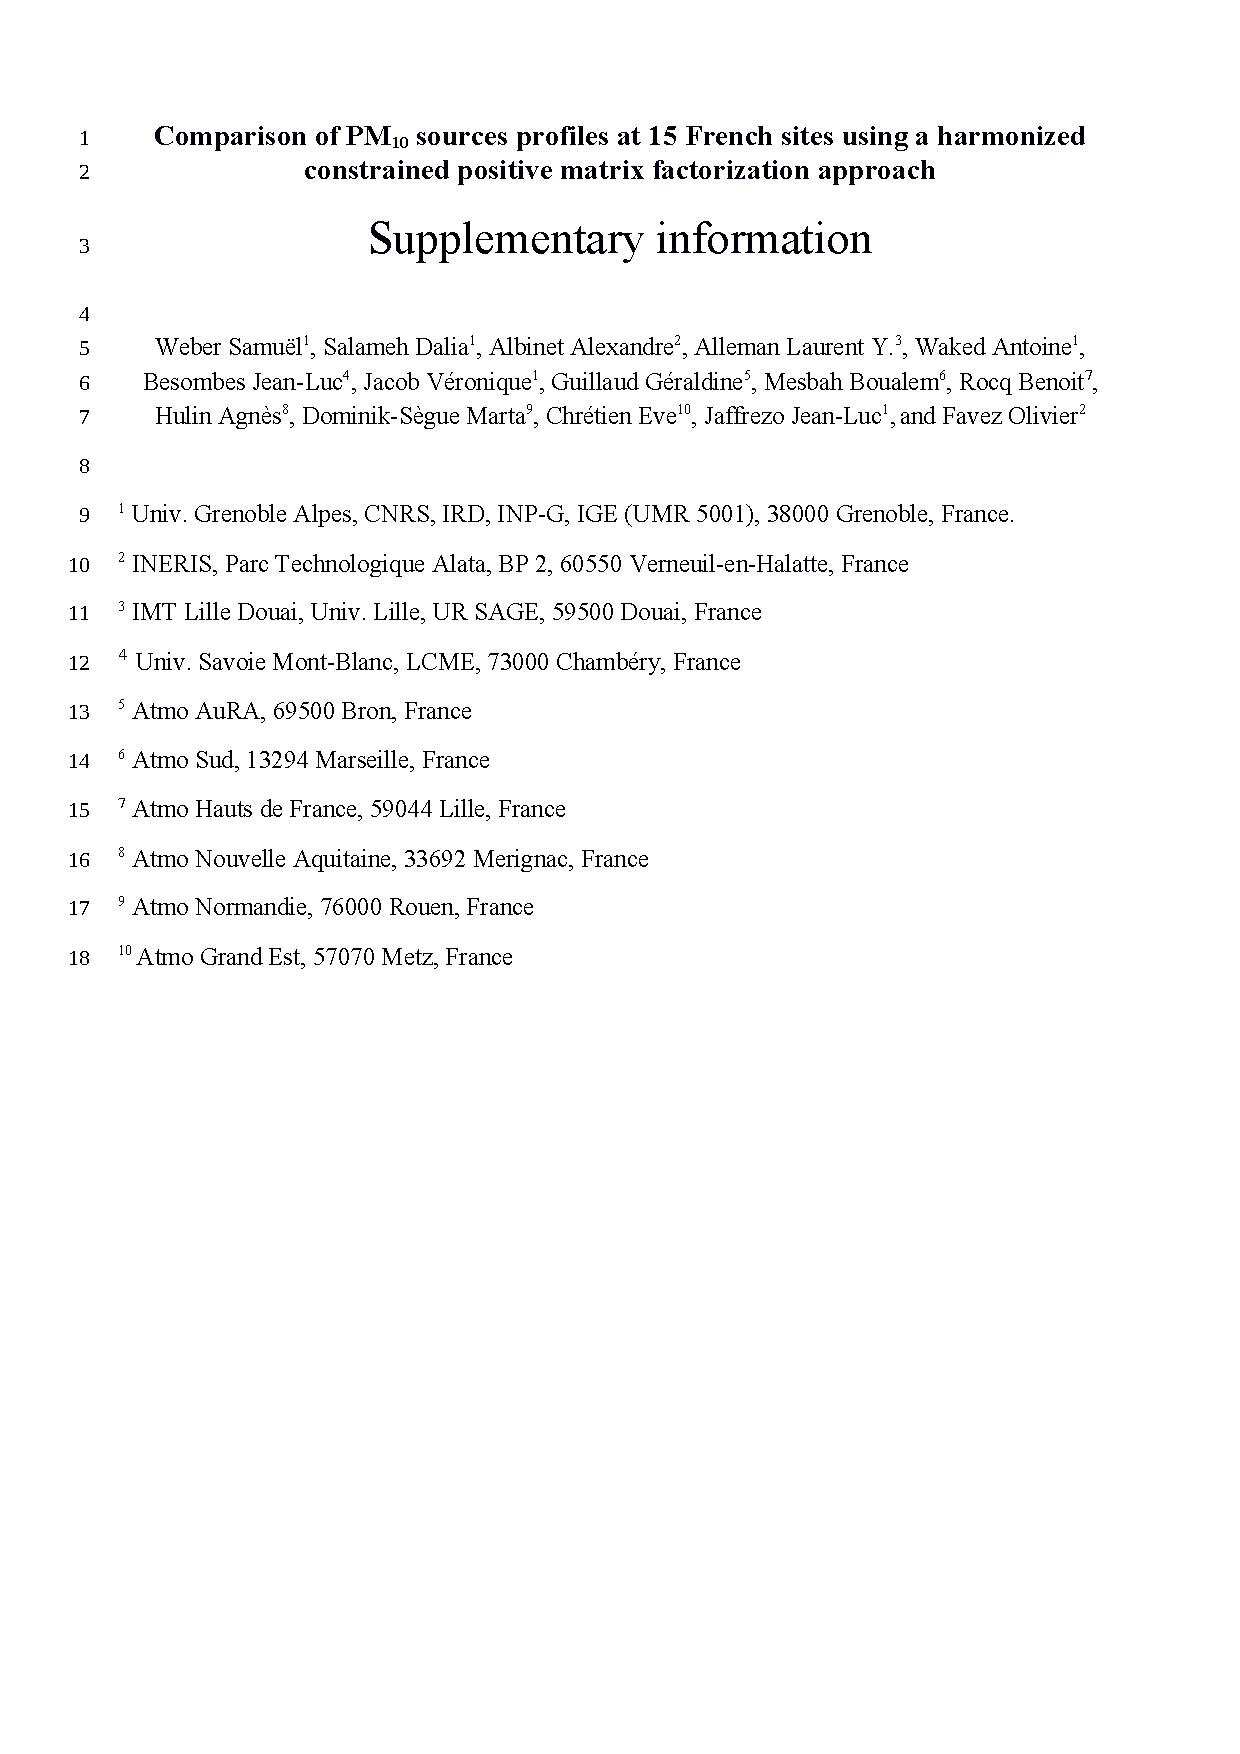
\includepdf[pages=-,scale=0.9,pagecommand={\pagestyle{fancy}}]{chapters/SOURCES_SI.pdf}


\section{Conclusion}%
\label{sec:conclusion}

Et aussi LCME: organique (BNT, hopane), EMPA cellulose PM10/PM2.5

Question : SPECIEUROPE et contrainte trop fortes sur certains profils ?

Ouverture : ANDRA et série temporelle

Limitation : 
- espèce trop réactive ? (oxalate ?)
- résolution temporelle




% \clearpage
% \printbibliography[segment=\therefsegment,heading=subbibliography]

\chapter{Estimation des sources de PO}
\label{cha:estimation_des_sources_de_PO}
\PartialToc
\clearpage
\nput{chapters/chapter04_methode_PO.tex}
\clearpage
\printbibliography[segment=\therefsegment,heading=subbibliography]

% \chapter{Passage à l'échelle régionale : application à 15 sites d'étude en France}
% \label{cha:application_to_15_sites_in_France}
% \PartialToc
% \clearpage
% \input{chapters/chapter05_synthese_PO.tex}
% \printbibliography[segment=\therefsegment,heading=subbibliography]

\chapter{Vers une modélisation spatialisé du PO}
\label{cha:spatio_temporal_modelizing}
% \PartialToc
% \clearpage
% \input{chapters/chapter06_spatialisation.tex}
% \printbibliography[segment=\therefsegment,heading=subbibliography]

% =====================================================================================
% Bibliographie complète {{{
% \addcontentsline{toc}{part}{Bibliography}
% \printbibheading
\printbibliography
% \bibbysegment[heading=subbibliography]

% }}}
% =====================================================================================

% =====================================================================================
% Appendix {{{
\addcontentsline{toc}{part}{Appendix}
\appendix
\setcounter{table}{0}
\setcounter{figure}{0}
\setcounter{equation}{0}
\renewcommand{\thetable}{\thesection-\arabic{table}}
\renewcommand{\thefigure}{\thesection-\arabic{figure}}
\renewcommand{\theequation}{\thesection-\arabic{equation}}

\section{INACS : isotopie et PMF}%
\label{annexe:INACS}
% \includepdf[pages=-,scale=0.95,pagecommand={\pagestyle{fancy}}]{chapters/annexerapportinacs2.pdf}

\section{SOURCES : complément d'information}
\label{annexe:SOURCES_SI}
% 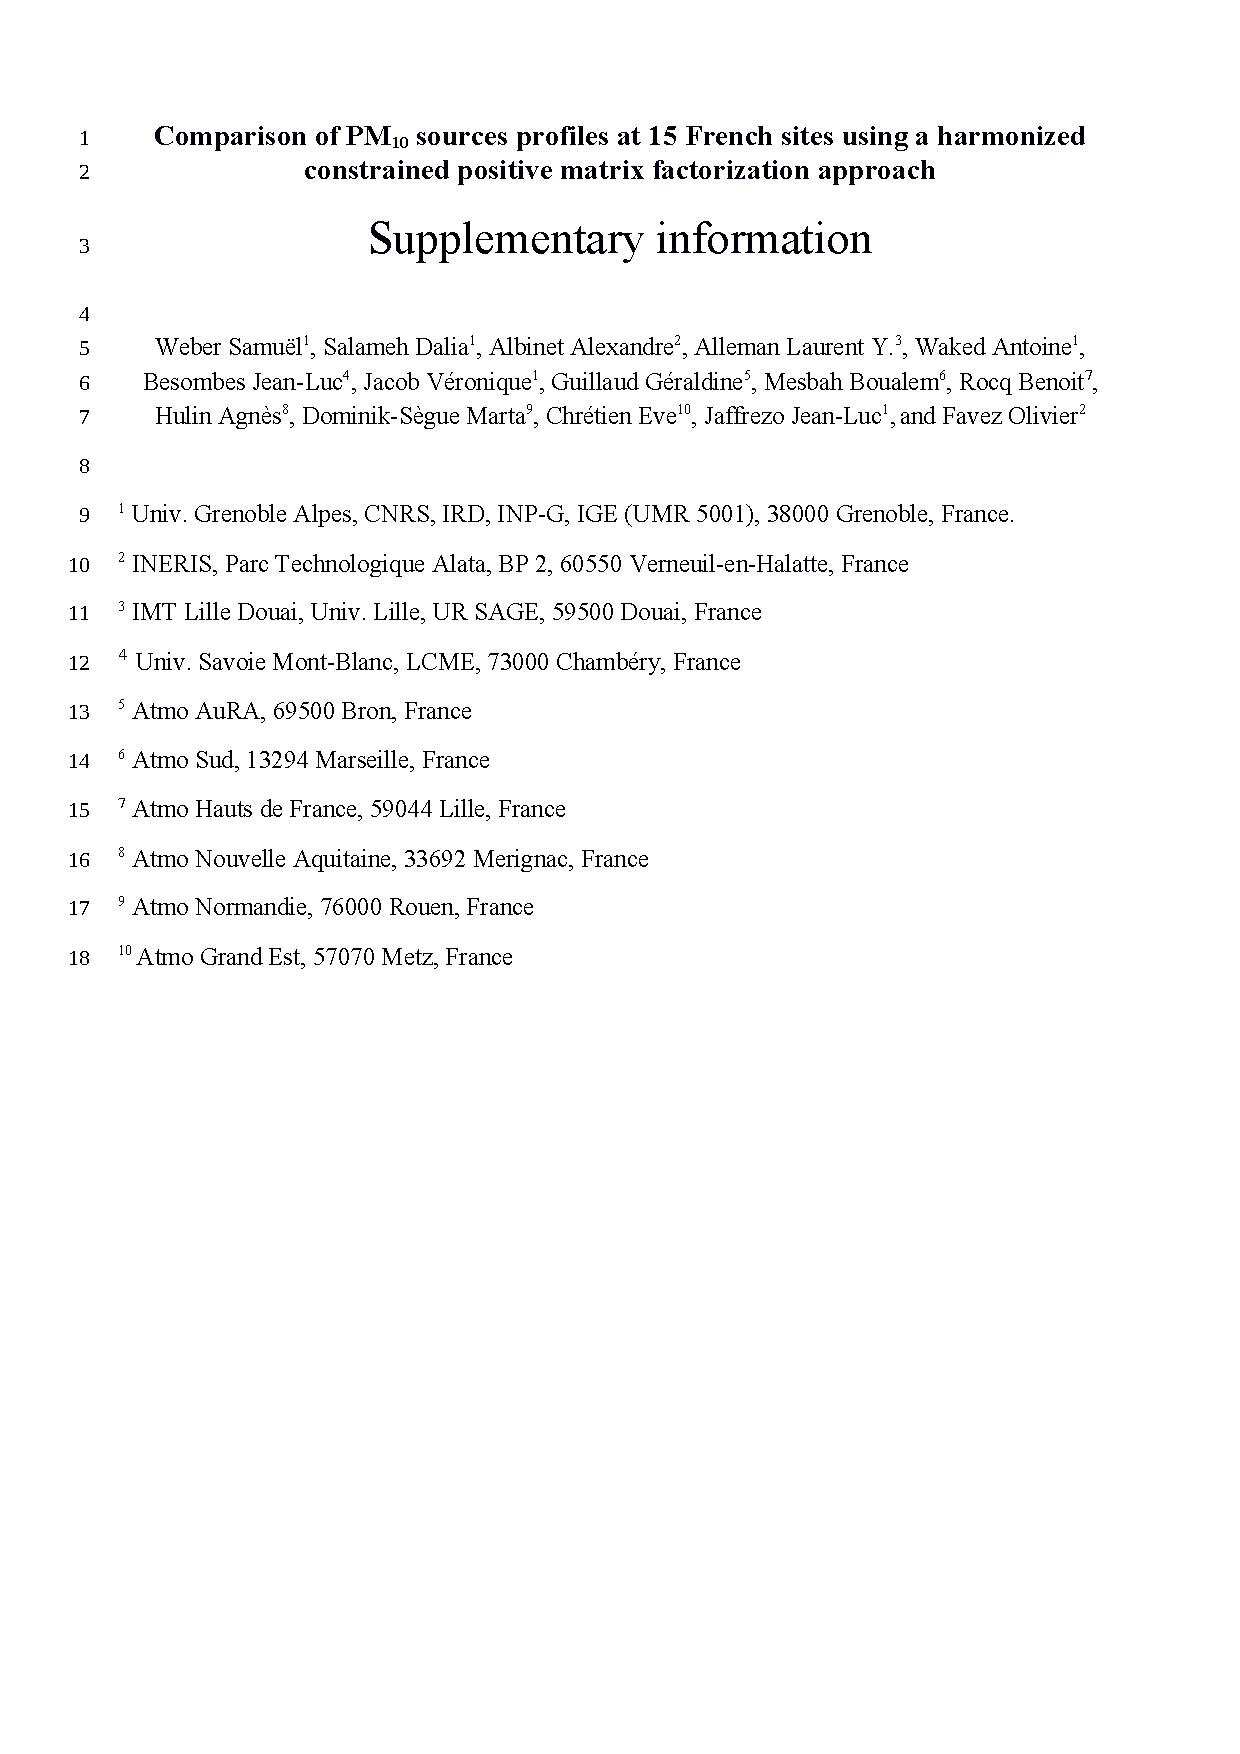
\includepdf[pages=-,scale=0.9,pagecommand={\pagestyle{fancy}}]{chapters/SOURCES_SI.pdf}

\section{Méthodologie de déconvolution du PO : complément d'information}
\label{annexe:deconvol_OP_SI}
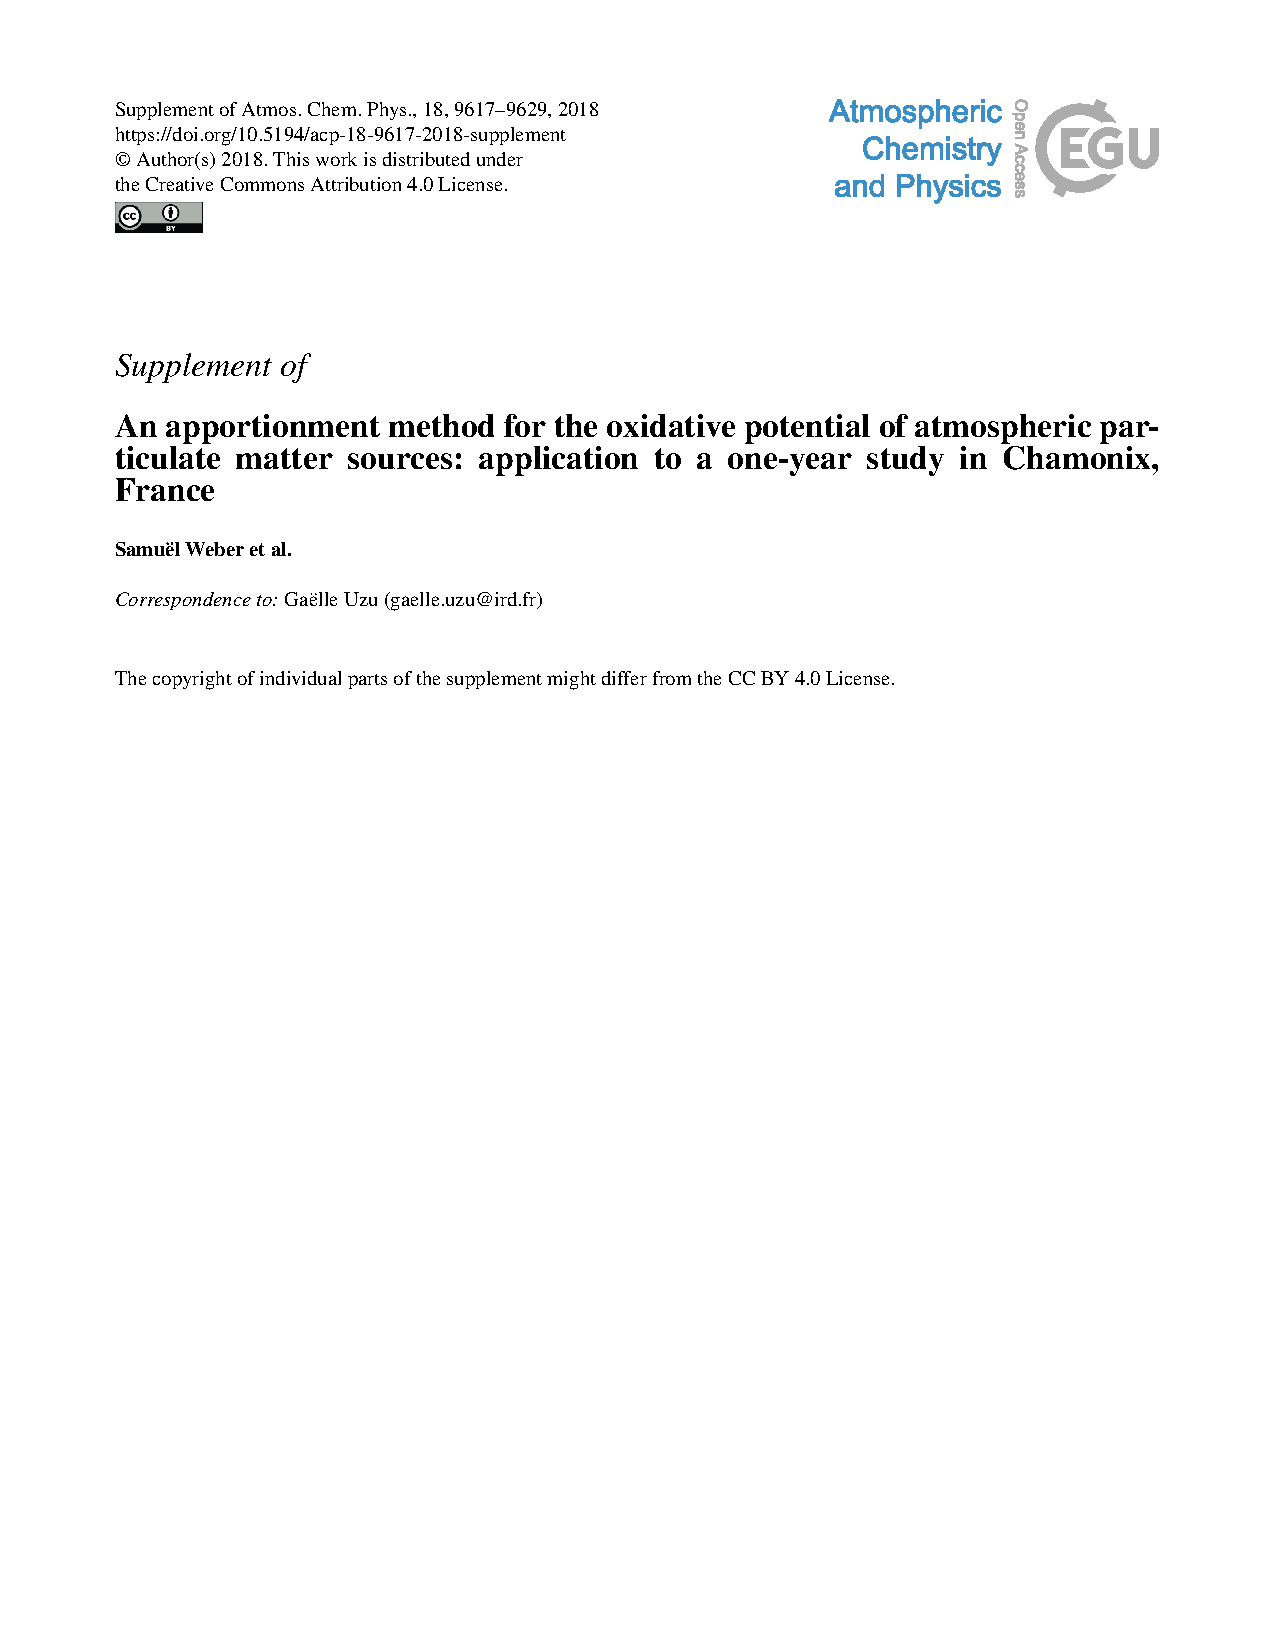
\includepdf[pages=-,scale=0.95,pagecommand={\pagestyle{fancy}}]{chapters/deconvol_OP_SI.pdf}

% }}}
% =====================================================================================
\end{document}
